% This template was originally by R. Jacob Vogelstein
% Updated on March 1, 2010 by Noah J. Cowan


\documentclass[12pt,oneside,final]{thesis}

\usepackage[superscript]{cite}
\usepackage{amsmath,amsfonts}
\usepackage{graphicx}
\graphicspath{{./figs/}}
\usepackage{fixltx2e}
\usepackage{array}
% wrapfig is fragile: use sparingly
\usepackage{wrapfig} 
%\usepackage{times}  % Use this for ugly fonts

\usepackage{upgreek}
\usepackage{hyperref}
\usepackage{setspace}

\usepackage{booktabs}
\usepackage{multirow}
\usepackage{longtable}
\usepackage[font=singlespacing, labelfont=bf]{caption}
\usepackage{gnuplot-lua-tikz}
\usepackage{subcaption}
\usepackage{minted}
\usepackage{algorithm}
\usepackage[noend]{algpseudocode}
\usepackage{listings}

\usepackage{enumitem}
\newlist{inlinelist}{enumerate*}{1}
\setlist*[inlinelist,1]{%
  label=(\arabic*),
}

\usepackage{fancyhdr}    % Use nice looking headers along with the required footer page numbers   
%\usepackage[hypertex]{hyperref}

%Define the header/footer style
\pagestyle{fancy}
\fancyhf{}
\setlength{\headheight}{15pt}
\lhead{\leftmark}
\cfoot{\thepage}
\renewcommand{\headrulewidth}{0pt}
\fancypagestyle{plain}{% Redefine ``plain'' style for chapter boundaries
\fancyhf{} % clear all header and footer fields
\fancyfoot[C]{\thepage} % except the center
\renewcommand{\headrulewidth}{0pt}
\renewcommand{\footrulewidth}{0pt}}
\newcommand{\para}[1]{\noindent{\bf #1:}}
\newcommand{\dz}[1]{{\color{blue}{\it DZ: #1}}}
\renewcommand{\algorithmicforall}{\textbf{for each}}

%\tolerance=10000

%\makeglossary % enable the glossary

\begin{document}

\title{FlashX: Massive Data Analysis Using Fast I/O}
\author{Da Zheng}
\degreemonth{Jul}
\degreeyear{2016} 
\dissertation
\doctorphilosophy
\copyrightnotice


% add your chapters, best way is to have separate TeX files for each chapter
%% FRONTMATTER
\begin{frontmatter}

% generate title
\maketitle

\begin{abstract}

With the explosion of data volume and the increasing complexity of data analysis,
large-scale data analysis imposes significant challenges in systems design.
While the current research focuses on scaling out
to a large clusters, these scale-out solutions introduce significant overheads.
This thesis is motivated by the advance of new I/O technologies such as flash
memory. Instead of scaling out, we explore efficient system designs in a single
commodity machine with non-uniform memory architecture (NUMA) and scale to large
datasets by utilizing commodity solid-state drives (SSDs). This thesis explores
the impact of the new I/O technologies in large-scale data analysis.
Instead of implementing individual data analysis algorithms for SSDs, we
develop a data analysis ecosystem called FlashX to target a large range of
data analysis tasks. FlashX includes three subsystems: SAFS, FlashGraph and
FlashMatrix. SAFS is a user-space filesystem optimized for a large SSD array
to deliver maximal I/O throughput from SSDs. FlashGraph is a general-purpose
graph analysis framework that processes graphs in a semi-external memory fashion
and scales to graphs with billions of vertices by utilizing SSDs through SAFS.
FlashMatrix is a matrix-oriented programming framework that supports both sparse
matrices and dense matrices for general data analysis. Similar to FlashGraph, it
scales matrix operations beyond memory capacity by utilizing SSDs. We demonstrate
that with the current I/O technologies FlashGraph and FlashMatrix in
the (semi-)external-memory meets or even exceeds state-of-the-art in-memory
data analysis frameworks while scaling to massive datasets for a large variety
of data analysis tasks.

\vspace{1cm}

\noindent Primary Reader: Some Person\\
Secondary Reader: Someone Else

\end{abstract}

\begin{acknowledgment}

Thanks!

\end{acknowledgment}

\begin{dedication}
 
This thesis is dedicated to \ldots

\end{dedication}

% generate table of contents
\tableofcontents

% generate list of tables
\listoftables

% generate list of figures
\listoffigures

\end{frontmatter}

\chapter{Introduction}
\label{sec:intro}
%\chaptermark{Optional running chapter heading}

% The key point here is that data is large and often irregular and we want
% to run complex computation on them.
In today's big data era, we face the challenges in both the explosion of
data volume and the increasing complexity of data analysis. Experiments,
simulations and observations generate terabytes or
even petabytes in many scientific and business areas. After collecting
a massive amount of data, we often need to perform complex data analysis
and machine learning techniques to gain insight from the data. Furthermore,
the fields of data analysis and machine learning evolve rapidly and the community
is developing many new algorithms to effectively extract value from massive
datasets.

% Graph analysis.
A class of commonly used data analysis in both academia and industry is graph
analysis. This models
real-world problems in the form of graphs (vertices and edges) to study objects
and the connection between the objects. Graph analysis becomes ubiquitous
and has applications to many fields such as social networks, semantic search
and knowledge discovery and cybersecurity. A well-known example is that Google
applies PageRank \cite{pagerank} on the Web page graph to determine the importance
of Web pages so that Google can provide users more relevant search results.

When applying graph analysis to real-world problems, we often encounter
massive and irregular graphs. For example, the Facebook social network graph
has billions of vertices, hundreds of billions of edges; the neural network
of a human brain has a fundamental size of $10^{11}$ vertices and $10^{15}$ edges;
graphs that evolve over time can grow even larger. These graphs often have
nearly random vertex connection and power law distribution, which cause random
memory access and load imbalance. As such, leading systems process graph analysis
in RAM and scale to large graphs in a cluster of machines. While good partitions
may be important for performance~\cite{surfer}, these leading systems partition
graphs randomly \cite{powergraph}. Network performance emerges as the bottleneck
and large-scale graph analysis requires fast networks to realize good performance.

% Matrix formulation for graph analysis
Although the lead graph processing frameworks view a graph as a collection of
vertices and edges, we can also represent a graph with a sparse matrix and
express graph analysis
as matrix operations \cite{Mattson13}. In this formulation, a row
or a column of a sparse matrix represents a vertex in a graph and a non-zero
entry encodes the existence of an edge or the edge weight on a graph.
As such, these matrices inherit structure from natural graphs. Specifically,
these matrices are typically very sparse and have near-random distribution
for non-zero entries. They also have a power law distribution that governs
the number of non-zero entries per row and column.

This matrix formulation has several advantages for some graph analysis problems.
First, this formulation is more intuitive for domain experts because users can
express their graph algorithms with high-level matrix operations. The matrix
formulation may also lead to more efficient implementations for some graph
analysis applications such as PageRank \cite{pagerank} and spectral clustering
\cite{spectral}, expressed intuitively with sparse matrix multiplication.
By highly optimizing this matrix operation, we significantly improve
performance of the implementations of many graph algorithms.

% Matrix formulation for general data analysis
Other than graph analysis, linear algebra is another fundamental tool for many
scientific and machine learning applications. In these applications, we store
data in (sparse or dense) matrices, and express algorithms with matrix
operations. Matrix formulation is simple and intuitive for domain experts.
This leads to the development of many popular matrix-oriented programming
frameworks, such as MatLab and R, to help scientists encode and deploy complex
algorithms.

Complex data analysis at a large scale faces significant challenges for
conventional tools. For instance, MatLab and R are known to scale to large
datasets poorly. Even though SQL database systems can process relatively large
datasets, their programming interface is not designed for programming machine
learning algorithms and their internal optimizations are not designed for this
type of workloads either.
The challenges lead to the redesign of data analysis tools.
MapReduce \cite{mapreduce} is one of the most well-known tools developed for
data analysis in the petabyte scale. Even though MapReduce is able to
process data of petabytes in a large cluster, the framework is not able to
handle many data analysis tasks efficiently due to the limited primitive
operations provided by the framework. Since then, many distributed frameworks,
such as Dryad \cite{dryad}, Spark \cite{spark} and Naiad \cite{naiad}, have
been developed for processing large datasets and these frameworks provides
more primitives to express data analysis algorithms more efficiently.
% related work in supercomputing.

Majority of the current research focuses on scaling out to a large cluster,
but many of them achieve better scalability at the cost of large overhead
introduced to the system. This is a common problem in many distributed systems
such as MapReduce. As McSherry et al. \cite{mcsherry15}
points out, many graph analysis frameworks such as PowerGraph \cite{powergraph}
and GraphX \cite{graphx} suffer from the same problem. As such, these systems
are less economical in terms of dollar efficiency and energy efficiency, which
are obstacles of moving to exascale computation.

% I/O
This thesis explores a different direction of scaling data analysis. Instead
of scaling out to a large cluster, we focus on large-scale data analysis in
a single machine, by utilizing the fast I/O technology, and explore
efficient implementations of data analysis tasks for a large parallel machine.

This work is motivated
by the tremendous improvement in storage I/O technology in the recent years.
For example, the latest development of flash memory \cite{fusionio, safs} has
reached over one million random IOPS and over ten gigabytes per second. This
is only one order of magnitude slower than RAM. We believe the advance of
I/O technologies opens a new direction for large-scale data analysis.
The tremendous performance
improvement in I/O potentially makes flash memory the true extension of RAM
and motivates us to develop new frameworks that fully utilize the I/O capacity
for large-scale data analysis.

% The goals of the dissertation.
Given the tremendous hardware improvement, this thesis addresses mainly two
questions: \textit{(i)} Can we replace RAM with fast flash memory in large-scale
data analysis? \textit{(ii)} To what extent
can the performance of flash-based data analysis approach that of RAM-based
data analysis? If data analysis on flash memory can achieve performance comparable to
that in RAM, it will positively affect computer architecture and revolutionize
large-scale data analysis.

In this thesis, we build
efficient programming frameworks with commodity hardware for various
data analysis applications such as graph analysis and machine learning.
%\dz{I need to emphasize the programming framework part.}
This work is orthogonal to the distributed solutions because our work serve as
a building block
for the distributed solutions to process data at even a larger scale.
% point out that our solution in some applications can outperform a pure
% distributed solution.

Hardware advances impose many new challenges in system design (both the operating
system and the data analysis framework). Operating systems were traditionally
designed with an assumption of slow I/O. There exists significant overhead in
almost all layers of the block stack of the Linux kernal when it operates on
fast storage. High-speed random I/O consumes significant CPU power, which
requires us to minimize CPU overhead for I/O access in order to maximize
the overall performance. Although the latest I/O devices deliver unprecedented
performance, they are still much slower than RAM, let alone CPU cache, in both
throughput and latency. As such, it is crucial for data analysis frameworks to
reduce I/O whenever
possible to achieve performance better than the raw hardware delivers.

% currsize is not set in the long table environment, so we need to set it before we set it up.
\makeatletter
\let\@currsize\normalsize
\makeatother

\begin{figure}[t]
\centering
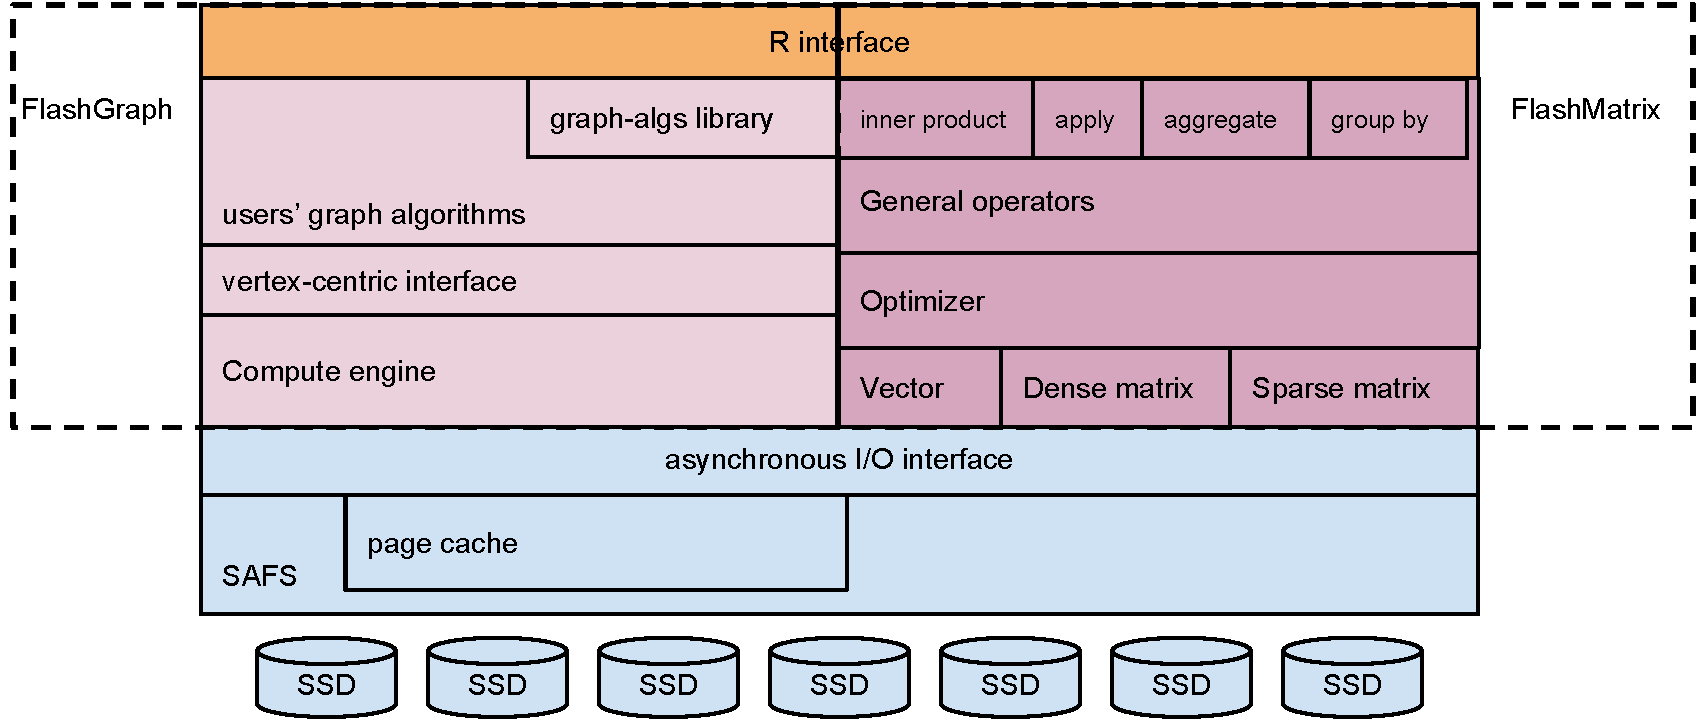
\includegraphics[scale=0.5]{figs/arch.pdf}
\label{fig:arch}
\caption{The architecture of FlashX.}
\end{figure}

We build an SSD-based data analysis ecosystem called FlashX to explore the benefits
that flash memory brings to large-scale data analysis. In this thesis,
we specifically targets graph analysis and machine learning due to their ubiquity.
FlashX has three main subsystems:
\begin{itemize}
	\item SAFS \cite{safs} is a user-space filesystem optimized for large SSD
		arrays. SAFS abstracts away the complexity of data access on SSDs and
		delivers the maximal I/O performance of a large SSD array in a NUMA
		machine. SAFS also provides an efficient caching layer \cite{SA-cache}.
	\item FlashGraph \cite{flashgraph} is a semi-external memory graph analysis
		framework. FlashGraph takes advantage of SAFS and issues I/O requests
		carefully to bring data from SSDs to CPUs efficiently for graph analysis
		to achieve performance comparable to in-memory counterparts. FlashGraph
		is specifically optimized for graph applications that generates random
		I/O access to SSDs.
	\item FlashMatrix implements a set of basic matrix operations as well as
		some generalized matrix operations to express a large range of machine
		learning and data analysis applications in external memory. It supports
		both sparse matrices \cite{SEM_SpMM} and dense matrices \cite{flashmatrix}.
		Like FlashGraph, the goal of FlashMatrix is to brings data from SSDs to
		CPUs efficiently for basic and generalized matrix operations. Unlike
		FlashGraph, FlashMatrix is optimized for applications with sequential
		I/O access to SSDs. FlashMatrix reimplements many matrix operations
		in the R framework to execute R code in parallel and out of core
		automatically.
\end{itemize}

FlashX uses semi-external memory for graph analysis
and matrix computation to achieve both scalability and computation efficiency.
For graph analysis, semi-external memory \cite{Abello98} maintains algorithmic
vertex state in RAM and edge lists on storage. Only using memory for vertices
increases the scalability of graph engines in proportion to the ratio of edges
to vertices in a graph. In FlashMatrix, we introduce a similar construct for
sparse matrix dense matrix multiplication in which one or more columns of
a dense matrix are kept in memory and the sparse matrix is accessed from
external memory. We can even extend this construct to some machine learning
algorithms such as k-means \cite{kmeans}, where some of the intermediate
computation state is kept in memory while input data matrices are stored on
SSDs. For many data analysis tasks, semi-external memory effectively utilizes
memory in a machine to reduce I/O access and achieve performance. In addition,
this computation paradigm reduces the amount of data written to SSDs
dramatically, which is essential to increase the lifetime of SSDs.

This thesis demonstrates that FlashX in semi-external memory realizes
in-memory performance for many data analysis tasks while scaling to massive
datasets in a single machine. FlashGraph in semi-external memory achieves
efficiency comparable to its in-memory version and Galois \cite{galois},
a high-performance, in-memory graph engine with a low-level API, on
a wide-variety of algorithms that generate diverse access patterns, while
significantly outperforming PowerGraph, a popular distributed in-memory
graph engine. We further demonstrate that FlashGraph can process massive
natural graphs in a single machine with relatively small memory footprint;
e.g., we perform breadth-first search on a graph of 3.4 billion vertices
and 129 billion edges using only 22 GB of memory. Similarly, the out-of-core
execution of FlashMatrix achieves performance comparable to the in-memory
execution. The implementations of machine learning algorithms in FlashMatrix
significantly outperforms the same algorithms in Spark MLlib \cite{mllib}.
FlashMatrix effortlessly scales to datasets with billions of data points and
its out-of-core execution uses a small fraction of resources required by
in-memory implementations. Given the fast performance and small memory footprint,
we conclude that FlashX offers unprecedented opportunities for users to perform
massive data analysis efficiently with commodity hardware.

\section{Related work}
% General-purpose data processing framework
MapReduce \cite{mapreduce} led the trend of large-scale data analysis. It
provides a very simple programming interface. Developers only need to provde
a \textit{map} function and
a \textit{reduce} function. The system scales users' computation to very large
datasets in a large cluster and handle machine failures automatically.
The simplicity of its programming interface and the unprecedented scalability
attracted tremendous academic and industrial attention, which leads to
the development of Hadoop \cite{hadoop}, the open-source clone of MapReduce.
MapReduce works very well for simple data processing tasks that can be
partitioned easily and do not require much communication between partitions.
Many data processing tasks at Google, such as count of URL access frequency
and reverse Web links, are tasks that fit the MapReduce programming paradigm.
However, if a task requires significant data exchange between partitions,
MapReduce requires sorting to move data to the right location, which leads
to significant overhead. As such, typical graph algorithms such as breadth-first
search and triangle counting are very slow in MapReduce.

Dryad \cite{dryad} and Naiad \cite{naiad} are distributed execution engine to
process
large datasets. Unlike MapReduce, Dryad provides a much more flexible computation
model and gives developers more fine-grain control over computation and data
communication. Developers construct a directed acyclic graph to describe
communication in the computation and define computation on the vertices in
the graph to express algorithms. Naiad provides an even more
flexible computation model, \textit{timely dataflow}, that supports data flow
graphs with loops. As such, it supports high throughput for batch processing,
low latency for stream processing as well as iterative and incremental
computations. Given the flexible computation model, both Dryad and Naiad
implement varieties of data processing tasks more efficiently at the cost of
higher programming complexity.

Unlike previous distributed frameworks, Spark \cite{spark} is specifically
optimized for in-memory data processing in a distributed environment.
Unlike MapReduce, which relies on writing data to the underlying distributed
filesystem to pass data reliably between MapReduce jobs, Spark keeps data
passed between different computation stages in memory
to avoid overhead of I/O access. Instead of replicating data to achieve
reliability, Spark stores transformation operations associated with RDDs to
reconstruct a lost partition of an RDD due to node failure.

% Programming interface on top of data processing frameworks
Due to the programming complexity in the distributed execution engines, many
programming frameworks have been developed on top of the distributed execution
engines. Pig Latin \cite{pig} and FlumeJava \cite{flumejava} build on top of
MapReduce to provide high-level SQL-like operations for general data analysis.
DryadLINQ \cite{dryadlinq} builds on top of Dryad and exposes a high-level
language to express data analysis tasks. Fundamentally, when these systems
translate high-level operations to low-level primitives, they combine high-level
operations to reduce the number of invocations of low-level primitives as much
as possible. The achievable performance of these programming frameworks is
bound by the underlying distributed execution engines.

% MapReduce-based systems for graph analysis and machine learning.
Given the popularity of MapReduce, many MapReduce-based systems have been
developed to perform graph analysis and machine learning tasks. PEGASUS
\cite{pegasus} is a popular graph processing engine built on MapReduce.
PEGASUS respects the nature of the MapReduce programming paradigm and
expresses
graph algorithms as a generalized form of sparse matrix-vector multiplication.
This form of computation works relatively well for graph algorithms such as
PageRank \cite{pagerank} and label propagation \cite{label_prop}, but performs
poorly for graph traversal algorithms. HEIGEN \cite{heigen} implements
an eigensolver on top of MapReduce for spectral analysis on billion-node
graphs. Despite optimizations in the framework, the HEIGEN eigensolver is
orders of magnitude slower than state-of-art distributed memory eigensolvers.
Cheng-Tao Chu et. al \cite{Chu07} implements a set of machine learning
algorithms using MapReduce to achieve speedup in a multicore machine. SystemML
\cite{systemml} builds a scalable declarative machine learning system on top
of MapReduce, which exposes a declarative higher-level language for writing
ML algorithms.

% Distributed graph processing frameworks
Due to the importance of graph analysis, both industry and academia build
dedicated graph processing frameworks for large-scale graph analysis.
Graph analysis results in a large number of random memory accesses, and
thus state-of-art graph engines use distributed memory for large-scale
graph analysis.
Pregel \cite{pregel} is a distributed graph-processing framework that
allows users to express graph algorithms in vertex-centric programs  
using bulk-synchronous processing (BSP).
It abstracts away the complexity of programming in a distributed-memory 
environment and runs users' code in parallel on a cluster.
Giraph \cite{giraph} is an open-source implementation of Pregel.
GraphLab \cite{graphlab} and PowerGraph \cite{powergraph} prefer shared-memory
to message passing and provide asynchronous execution.
Trinity \cite{trinity} optimizes message passing by restricting vertex
communication to a vertex and its direct neighbors.

% External-memory graph processing frameworks
Despite random memory access required by graph analysis, significant efforts
have been made to scale graph analysis using disks. GraphChi \cite{graphchi}
and X-stream \cite{xstream} are specifically designed for magnetic disks. They
eliminate random data access from disks by scanning the entire graph dataset
in each iteration. Like graph processing frameworks built on top of MapReduce,
they work relatively well for graph algorithms that require computation on all
vertices, but share the same limitations, i.e., suboptimal graph traversal
algorithm performance. TurboGraph \cite{turbograph} is an external-memory graph
engine optimized for SSDs. TurboGraph targets graph algorithms
expressed in sparse matrix vector multiplication, so it is difficult to
implement graph applications such as triangle counting.

% linear algebra for graph analysis
Many graph algorithms can be formulated as sparse matrix multiplication or
generalized sparse matrix multiplication \cite{Mattson13, linear_algebra}.
In this abstraction, PageRank and label propagation are efficiently expressed
as sparse-matrix, dense-vector multiplication, and breadth-first search as 
sparse-matrix, sparse-vector multiplication. KDT \cite{kdt} is a system that
realizes the abstraction and performs graph analysis using linear algebra with
sparse adjacency matrices and vertex-state vectors as data representations.
These frameworks target mathematicians and those with the ability to formulate
and express their problems in the form of linear algebra.

% Additional frameworks for large-scale machine learning.
Many machine learning frameworks have been developed to enable large-scale
machine learning. H2O \cite{h2o} and Spark MLlib \cite{mllib} are machine
learning libraries with a collection of machine learning algorithms implemented
on Spark. GraphLab \cite{graphlab} is a programming framework that provides
primitives for graph-based machine learning algorithms in a distributed
environment. OptiML \cite{optiml} is a domain-specific language and supports
vector, matrix and graph operations to implement machine learning algorithms.
It is built on top of a parallel runtime system called Delite \cite{delite}
to enable parallelism in a heterogeneous computation environment in a single
machine. Petuum \cite{petuum} is a distributed programming framework for
implementing machine learning algorithms. It leverages several fundamental
properties of machine learning algorithms: error tolerance, dynamic structure
and non-uniform convergence, and aims at faster convergence of
an algorithm instead of achieving higher throughput in a single iteration.

\chapter{Set-associative filesystem (SAFS)}
\label{sec:safs}
\chaptermark{}

We describe a storage system that 
removes I/O bottlenecks to achieve more than one million IOPS
based on a user-space file abstraction for arrays of commodity SSDs.
The file abstraction refactors I/O scheduling and placement for extreme
parallelism and non-uniform memory and I/O.
The system includes a set-associative, parallel page cache in the user space.
We redesign page caching to eliminate CPU overhead and lock-contention in non-uniform memory
architecture machines.
We evaluate our design on a 32 core NUMA machine with four, eight-core processors. 
Experiments show that our design delivers 1.23 million 512-byte read IOPS.
The page cache realizes the scalable IOPS of Linux asynchronous I/O (AIO) 
and increases
user-perceived I/O performance linearly with cache hit rates.
The parallel, set-associative cache matches the cache hit rates
of the global Linux page cache under real workloads.

\section{Introduction}

Systems that perform fast, random I/O are revolutionizing commercial data
services and scientific computing, creating the capability to quickly 
extract information from massive data sets \cite{4thparadigm}.  
For example, NoSQL systems underlying cloud stores generate
small, incoherent I/Os that search key indexes and reference values, tables, documents,
or graphs.  The design of Amazon's DynamoDB testifies to this trend; it differentiates
itself as a fast and scalable technology based on integrating SSDs
into a key/value database~\cite{dynamodb}.  In scientific computing, SSDs improve the throughput 
of graph and network analyses by an order of magnitude over magnetic disk \cite{Pearce10}.
Data sets that describe graphs are notoriously difficult
to analyze on the steep memory hierarchies of conventional HPC hardware 
\cite{Hendrickson09}, because they induce fine-grained, incoherent data accesses.
The future of data-driven computing will rely on extending random access to large-scale 
storage, building on today's SSDs and other non-volatile memories as they emerge.

Specialized hardware for random access offers an effective solution,
albeit costly.  For example, Fusion-IO provides 
NAND-flash persistent memory that delivers over one million accesses per second.
Fusion-IO represents a class of persistent memory devices that are used as 
application accelerators integrated as memory addressed directly from the processor.  
As another approach, the Cray XMT architecture implements a flat memory system so 
that all cores have fast access to all memory addresses.  This approach
is limited by memory size.  All custom hardware approaches cost multiples of commodity SSDs.

While recent advances in commodity SSDs have
produced machines with hardware capable of over one million random IOPS,
standard system configurations fail to realize the full potential 
of the hardware. 
Performance issues are ubiquitous in hardware and software, ranging from the assignment of interrupts, to non-uniform
memory bandwidth, to lock contention in device drivers and the operating system.
Problems arise because I/O systems were not designed for the extreme
parallelism of multicore processors and SSDs.  The design of file systems, page caches, device
drivers and I/O schedulers does not reflect the parallelism (tens to hundreds of contexts)
of the threads that initiate I/O or the multi-channel devices that service I/O requests.

%These systems have the potential to revolutionize commercial data services and scientific computing
%by creating . For instance, cloud data services
%such as key/value store and other NoSQL database requires many index lookups,
%which generates many small I/O accesses. Graph database needs to fetch
%many vertices and edges scattered in different locations in external
%memory while processing queries. Random I/O has become an important performance
%factor \cite{Muth11}.

%$\rb{some words about the brain DB and its workload}
%$
%\rb{What applications require intensive random writes?}

None of the I/O access methods in Linux kernel perform well on a high-speed SSD array.
%The current block subsystem in Linux kernel is fairly heavyweight \cite{}
%so that an 
I/O requests go through many layers in the kernel before reaching a device \cite{Foong10}.
This produces significant CPU consumption under high IOPS.
Each layer in the block subsystem uses locks to protect its data
structures during concurrent updates. Furthermore, SSDs require many parallel
I/Os to achieve optimal performance, while synchronous I/O, 
such as buffered I/O and direct I/O, issues one I/O request per thread at a time.
The many threads needed to load the I/O system produce lock contention
and high CPU consumption.
%, so they need to
%use many threads to issue requests in parallel, which leads to poor
%performance and tremendous CPU consumption. 
%
Asynchronous I/O (AIO), which issues multiple requests in a single thread, provides a better
option for accessing SSDs. However, AIO does not integrate with the operating 
system page cache so that SSD throughput limits user-perceived performance.

% RB HERE
The goal of our system design is twofold: (1) to eliminate bottlenecks in parallel I/O 
to realize the full potential of SSD arrays and (2) to integrate caching into SSD I/O to amplify the 
user-perceived performance to memory rates.  
Although the performance of SSDs has advanced in the past years, it
does not approach memory both in random IOPS or latency (Table \ref{ssd}). 
Furthermore, RAM may be accessed at a finer granularity 64 versus 512 bytes, which can widen the performance gap 
by another factor of eight for workloads that perform small requests.
We conclude that SSDs require a memory page cache interposed between an SSD file system and applications.
This is in contrast to translating SSD storage into the memory address space using direct I/O. % \cite{directio}.
A major obstacle to overcome is that the page caches in operating systems do not scale to millions of IOPS.
They were designed for magnetic disks that perform only about 100 IOPS per device.
Performance suffers as access rates increase owing to lock contention 
and with increased mutli-core parallelism owing to processor overhead.

%Such devices 
%can be operated as block storage devices \cite{vsl}, but then must 
%integrated with the standard operating system.

%, but it is not commonly adopted due to its
%high price. Instead, we can build a high-speed storage device with low
%price by combining many commodity SSDs, which can also deliver over one
%million IOPS. However, one may not gain one million IOPS by simply attaching
%%many SSDs to a multi-core computer. It turns out to be a non-trivial task
%to achieve optimal performance from many SSDs on a single machine.

%DZTODO what to do with this citation?
%Random I/O has become an important performance factor \cite{Muth11}.


%DFS \cite{dfs} is such an effort to redesign the file system to tackle the problem. 
%However, we choose to utilize current
%file systems in the Linux kernel and provide a single file system interface
%on top of an SSD array in the user space. We show that by accessing underlying
%Linux file systems properly, we can achieve the same read/write performance
%as raw devices.

The first contribution of this paper is the design of a user-space file abstraction that
performs more than one million IOPS on commodity hardware.   We implement a thin software
layer that gives application programmers synchronous and asynchronous interfaces to 
file I/O.  The system modifies I/O scheduling, interrupt handling, and data placement
to reduce processor overhead, eliminate lock contention, 
and account for affinities between processors, memory, and storage devices.

We further present a scalable user-space cache for NUMA machines and
arrays of SSDs that realizes I/O
performance of Linux asynchronous I/O for cache misses and preserve the 
cache hit rates of the Linux page cache under real workloads. 
Our cache design is set-associative; it breaks
the page buffer pool into a large number of small page sets and
manages each set independently to reduce lock
contention. The cache design extends to NUMA architectures by
partitioning the cache by processors and using message passing for
inter-processor communication.

The evaluation on a 32 core NUMA machine shows promising results. Our design
delivers 1.23 million 512-byte read IOPS with our current hardware.
The page cache realizes the scalable IOPS of
Linux asynchronous I/O (AIO) and increases user-perceived I/O performance
linearly with cache hit rates. To demonstrate the performance of our system
in a typical HPC environment, we integrate it into the IOR benchmark \cite{IOR},
a popolar HPC benchmark for I/O performance. The IOR benchmark further shows
our design achieves good performance for all request sizes and the synchronous
write in our system performs nearly as well as asynchronous write.

%The contribution of our work is mainly in three folds: we build an SSD RAID with
%low-cost hardware and a thin software layer, capable of delivering performance
%comparable to the fastest Fusion-IO; we design and implement a low-overhead
%and scalable cache both on a multi-core SMP machine and a NUMA machine, optimized
%for both workloads with low cache hit ratio and with high cache hit ratio; we
%compare our cache design with several optimized lock-free cache designs and
%show the performance of our cache is superior to the lock-free caches.

\begin{table}
\begin{center}
\small
\begin{tabular}{|c|c|c|c|}
\hline
& random IOPS & latency & granularity \\
\hline
ioDrive Octal \cite{fusion} & 1,300,000 & 45$\mu$s &512B \\
\hline
OCZ Vertex 4 \cite{ocz} & 120,000 & 20$\mu$s & 512B \\
\hline
DDR3-1333 & 7,300,000 & 15ns & 64B \\
\hline
\end{tabular}
\normalsize
\end{center}
\caption{The performance of specialized memory-addressable NAND flash (ioDrive Octal), a commodity SSD (OCZ Vertex 4), and memory (DDR3-1333). 
IOPS are measured with 512-byte random accesses.}
\label{ssd}
\end{table}

\section{Related work}

This research falls into the broad area of the scalability operating systems
with parallelism.  Several research efforts \cite{fos, barrelfish} treat a
multicore machine as a network of independent cores and implement OS
functions as a distributed system of processes that communicate with message passing.
We embrace this idea for processors and hybridize it with traditional SMP programming models
for cores.  Specifically, we use shared memory for communication inside a processor 
and message passing between processors.

As a counterpoint, a team from MIT \cite{mit_scale} conducted a comprehensive
survey on the kernel scalability and concluded that the traditional monolithic
kernel can also have good parallel performance.  We demonstrate that this is 
not the case for the page cache at millions of IOPS.

More specifically, our work relates to the scalable page cach\-ing.
Yui et al. \cite{nbgclock} designed a lock-free cache management for database
based on Generalized CLOCK \cite{gclock} and use a lock-free hashtable as index.
They evaluated their design in a eight-core computer.
%Lock-free implementations work well when contention is low. For caching,
%this corresponds to high-hit rates.
We provide an alternative
design of scalable cache and evaluate our solution at a larger scale.

The open-source community has improved the scalability of Linux page cache.
Read-copy-update (RCU) \cite{rcu} reduces contention through lock-free synchronization 
of parallel reads from the page cache (cache hits).  However, the Linux kernel still 
relies on spin locks to protect page cache from concurrent updates (cache misses).
In contrast, our design focuses on random I/O, which implies a high churn rate
of pages into and out of the cache.

Park et al. \cite{park09} evaluated the performance effects of SSDs on scientific
I/O workloads and they used workloads with large I/O requests. They concluded that 
SSDs can only provide modest performance gains over mechanical hard drives.
As the advance of SSD technology, the performance of SSDs have been improved
significantly, we demonstrate that our SSD array can provide random and sequential
I/O performance many times faster than mechanical hard drives to accelerate
scientific applications.

The set-associative cache  was originally inspired by theoretical results 
that shows that a cache with restricted associativity can approximate LRU \cite{Sen02}.
We build on this result to create a set-associative cache that matches the 
hit rates of the Linux kernel in practice.

The high IOPS of SSDs have revealed many performance issues with 
traditional I/O scheduling, which has lead to the development of 
new fair queuing techniques that work well with SSDs \cite{Park12}.
We also have to modify I/O scheduling as one of many optimizations to 
storage performance.

Our previous work \cite{hotstorage12} shows that a fixed size set-associative cache
achieves good scalability with parallelism using a RAM disk.
This paper extend this result to SSD arrays and adds features, such as replacement,
write optimizations, and dynamic sizing.  The design of the user-space file abstraction
is novel to this paper as well.

\section{A High IOPS File Abstraction}

Although one can attach many SSDs to a machine, 
it is a non-trivial task to  aggregate the performance of all SSDs.
The default Linux configuration delivers only a fraction of optimal
performance owing to skewed interrupt distribution, device affinity
in the NUMA architecture, poor I/O scheduling, and lock contention
in Linux file systems and device drivers.
The process of optimizing the storage system to realize the 
full hardware potential includes setting configuration parameters,
the creation and placement of dedicated threads that perform I/O,
and data placement across SSDs.  
Our experimental results demonstrate that our design
improves system IOPS by a factor of 3.5.

\subsection{Reducing Lock Contention}

Parallel access to file systems exhibits high lock contention. 
Ext3/ext4 holds an exclusive lock on an inode, a data structure
representing a file system object in the Linux kernel, for both reads and
writes.  For writes, XFS holds an exclusive lock on each inode that 
deschedules a thread if the lock is not immediately available. 
In both cases, high lock contention causes significant CPU overhead or,
in the case of XFS, frequent context switch, and prevents the file systems
from issuing sufficient parallel I/O.
Lock contention is not limited to the file system, the kernel has
shared and exclusive locks for each block device (SSD).

To eliminate lock contention, we create a dedicated thread
for each SSD to serve I/O requests and use asynchronous I/O (AIO)
to issue parallel requests to an SSD.
Each file in our system consists of multiple individual 
files, one file per SSD, a design similar to PLFS \cite{plfs}.
By dedicating an I/O thread per SSD, the thread
owns the file and the per-device lock exclusively at all time.
There is no lock contention in the file system and block devices.
AIO allows the single thread to output multiple I/Os at the same time.
The communication between application threads and I/O threads is
similar to message passing. An application thread sends requests to an I/O 
thread by adding them to a rendezvous queue. The add operation
may block the application thread if the queue is full. Thus, the 
I/O thread attempts to dispatch requests immediately upon arrival. 
Although there is locking in the rendezvous queue, the locking overhead
is reduced by the two facts: each SSD maintains its own message queue,
which reduces lock contention; the current implementation bundles
multiple requests in a single message, which reduces the number of
cache invalidations caused by locking.

\subsection{Processor Affinity}

Non-uniform performance to memory and the PCI bus throttles IOPS
owing to the inefficiency of remote accesses.
In recent multi-processor machines for both AMD and Intel architectures,
each processor connects to its own memory and PCI bus.  The memory and
PCI bus of remote processors are directly addressable, but at increased
latency and reduced throughput. 

We avoid remote accesses by binding I/O threads to the processors 
connected to the SSDs that they access.
This optimization leverages our 
design of using dedicated I/O threads, making it possible to localize all 
requests, regardless of how many threads perform I/O.  
By binding threads to processors, we ensure that all I/Os are sent to the 
local PCI bus.

\begin{figure}[t]
\centering
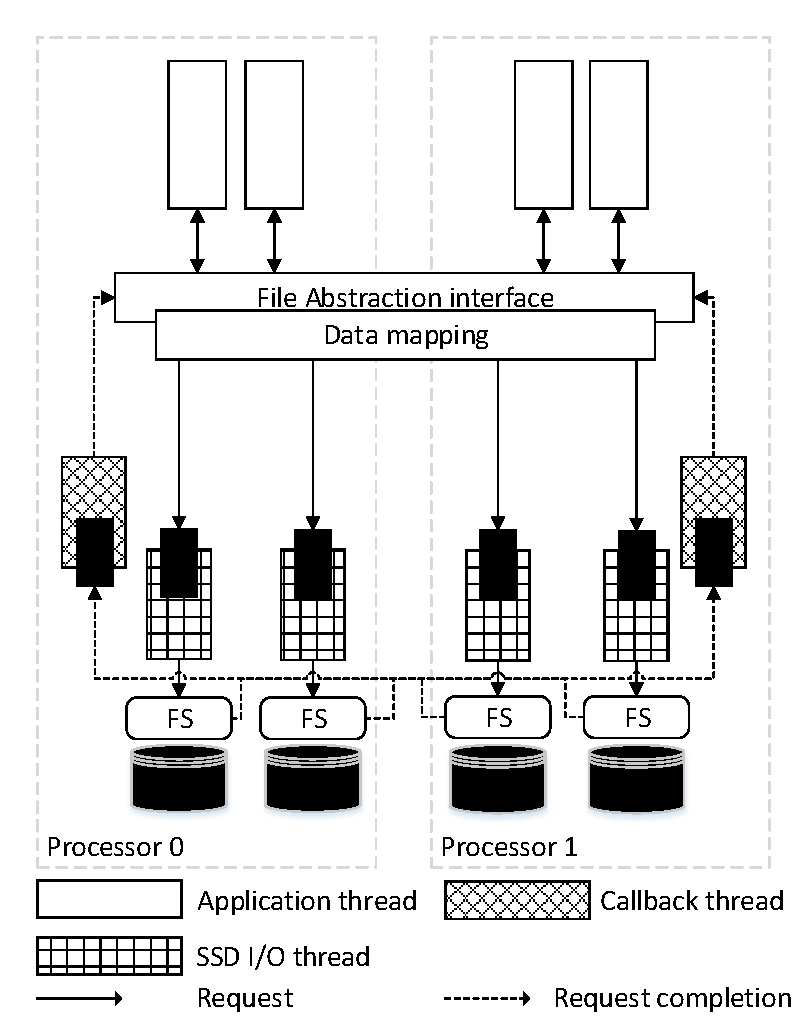
\includegraphics[scale=0.6]{figs/SAFS/SSD-array.pdf}
\vspace{-5pt}
\caption{The architecture of the SSD file abstraction (SSDFA).}
\vspace{-5pt}
\label{SSD_VFS}
\end{figure}

\subsection{Other Optimizations}

\para{Distributing Interrupts}
With the default Linux setting, interrupts from SSDs are not evenly distributed
among processor cores and we often witness that all interrupts are sent to a single core. 
Such large a number of interrupts saturates a CPU core which throttles system-wide
IOPS.

We remove this bottleneck by distributing interrupts evenly among all 
physical cores of a processor using the message signalled interrupts extension to 
PCI 3.0 (MSI-X) \cite{msix}.  MSI-X allows devices to select targets for up 
to 2048 interrupts.  We distribute the interrupts of a storage controller 
host-bus adapter across multiple cores of its local processor.

\para{I/O scheduler}
Completely Fair Queuing (CFQ), the default I/O scheduler in the Linux kernel >2.6.18,
maintains I/O requests in per-thread queues and allocates time slices for each process
to access disks to achieve fairness. 
When many threads access many SSDs simultaneously, CFQ prevent threads 
from delivering sufficient parallel requests to keep SSDs busy.
Performance issues with CFQ and SSDs have lead researchers to redesign 
I/O scheduling \cite{Park12}. Future Linux releases plan to include new schedulers.

At present, there are two solutions.  The most common is to use the 
noop I/O scheduler, which does not perform per-thread
request management.  This also reduces CPU overhead.  Alternatively, accessing
an SSD from a single thread allows CFQ to inject sufficient requests.
Both solutions alleviate the bottleneck in our system.  

\para{Data Layout}\label{data_layout}
To realize peak aggregate IOPS, we parallelize I/O among all SSDs by 
distributing data.  We offer three data distribution functions implemented in 
the data mapping layer of Figure \ref{SSD_VFS}.

\vspace{-10pt}
\begin{itemize}
\addtolength{\itemsep}{-5pt}
	\item Striping: Data are divided into fixed-size small blocks placed on 
    successive disks in increasing order.  This layout is most efficient
    for sequential I/O, but susceptible to hotspots.
	\item Rotated Striping: Data are divided into stripes but the start disk for
    each stripe is rotated, much like distributed parity in RAID5 \cite{raid}.
    This pattern prevents strided access patterns from skewing the workload
    to a single SSD.
	\item Hash mapping: The placement of each block is randomized
    among all disks.  This fully declusters hotspots, but requires each
    block to be translate by a hash function.
\end{itemize}
\vspace{-10pt}

\noindent Workloads that do not perform sequential I/O benefit from randomization.

\subsection{Implementation}
We implement this system in a user-space library that exposes a simple
file abstraction (SSDFA) to user applications. It supports basic operations
such as file creation, deletion, open, close, read and write,
and provides both synchronous and asynchronous read and write interface.
Each virtual file has metadata to keep track of the corresponding files on the
underlying file system. Currently, it does not support directories.

The architecture of the system is shown in Figure \ref{SSD_VFS}.
It builds on top of a Linux native file system on each SSD.
Ext3/ext4 performs well in the system as does XFS, which we use in experiments. 
Each SSD has a dedicated I/O thread to process application requests.
On completion of an I/O request, a notification is sent to a dedicated callback
thread for processing the completed requests. The callback threads help to
offload computation in the I/O threads and help applications to achieve processor
affinity. Each processor has a callback thread.

\section{A Set-Associative Page Cache}

The emergence of SSDs has introduced a new performance bottleneck into
page caching: managing the high churn or page turnover associated with
the large number of IOPS supported by these devices. Previous efforts
to parallelize the Linux page cache focused on parallel read throughput
from pages already in the cache. For example, read-copy-update (RCU) \cite{rcu}
provides low-overhead wait free reads from multiple threads. This supports
high-throughput to in-memory pages, but does not help address high page
turnover.

Cache management overheads associated with adding and evicting pages in
the cache limit the number of IOPS that Linux can perform. The problem lies
not just in lock contention, but delays from the L1-L3 cache misses during
page translation and locking.
We redesign the page cache to eliminate lock and
memory contention among parallel threads by using set-associativity.
The page cache consists of many small sets of pages (Figure \ref{cache_struct1}).
A hash function maps each logical page to a set in which it can occupy
any physical page frame. 
%The same hash function as in the SSD virtual file
%system is used, but with a larger $p$.

We manage each set of pages independently using a single lock and no lists.
For each page set, we retain a small amount of metadata to describe the page
locations. We also keep one byte of frequency information per page.
We keep the metadata of a page set in one or few cache lines to minimize
CPU cache misses. If a set
is not full, a new page is added to the first unoccupied position. Otherwise,
a user-specified page eviction policy is invoked to evict a page.
The current available eviction policies are LRU, LFU, Clock \cite{clock} and
GClock \cite{gclock}.

%Small page sets keeps metadata (counters and occupancy) . The total metadata for eight pages is
%208 bytes without non-resident pages enabled. This and the metadata for 37
%non-resident pages fits within 4 128-byte cache lines. \dz{Recalculate the numbers here.}

As shown in figure \ref{cache_struct1}, each page contains a pointer to
a linked list of I/O requests. When a request requires a page for which an
I/O is already pending, the request will be added
to the queue of the page. Once I/O on the page is complete, all requests in
the queue will be served. 
%The request queue can is alalso help deal with the case
%of evicting a dirty page, as described in section \ref{rw_opt}.

There are two levels of locking to protect the data structure of the cache:
\vspace{-10pt}
\begin{itemize}
\addtolength{\itemsep}{-5pt}
\item per-page lock: a spin lock to protect the state of a page.
\item per-set lock: a spin lock to protect search, eviction, and replacement
   inside a page set.
\vspace{-10pt}
\end{itemize}
\noindent A page also contains a reference count that prevents a page from
being evicted while the page is being used by other threads.

\begin{figure}[t]
\centering
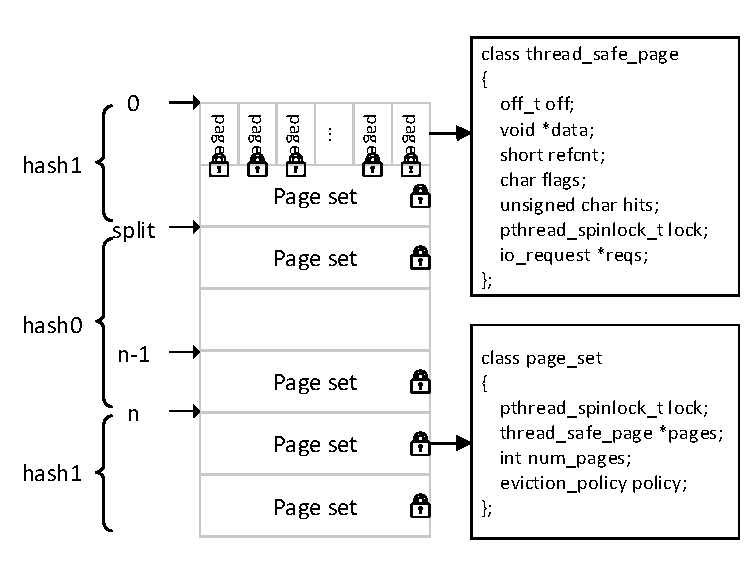
\includegraphics[scale=0.7]{figs/SAFS/SA-cache.pdf}
\vspace{-5pt}
\caption{The organization of the set-associative cache showing the data structures
and locks for pages and page sets.  The hash0 and hash1 functions 
implement linear hashing \cite{linear_hash} used to resize the cache.
$n = init\_size \times 2^{level}$.}
\vspace{-5pt}
\label{cache_struct1}
\end{figure}


\subsection{Resizing}

A page cache must support dynamic resizing to share physical memory with
processes and swap.  We implement dynamic resizing of the cache with 
linear hashing \cite{linear_hash}.  
Linear hashing proceeds in rounds that double or halve
the hashing address space. The actual 
memory usage can grow and shrink incrementally.  
We hold the total number of allocated pages through loading and eviction
within the page sets.
When splitting a page set $i$, we rehash its pages 
to set $i$ and $init\_size \times 2^{level}+i$. 
The number of page sets
is defined as $init\_size \times 2^{level} + split$. \textit{level} indicates
the number of times that pages have been split.  
\textit{split} points to the page set to be split. 
The cache uses two hash functions within each level \textit{hash0} and \textit{hash1}:
\vspace{-10pt}
\begin{itemize}
  \addtolength{\itemsep}{-5pt}
	\item $hash0(v) = h(v, init\_size \times 2^{level})$
	\item $hash1(v) = h(v, init\_size \times 2^{level + 1})$
\end{itemize}
\vspace{-10pt}
If the result of \textit{hash0} is smaller than \textit{split}, \textit{hash1}
is used for the page lookup as shown in figure \ref{cache_struct1}.

\subsection{Read and write optimizations}\label{rw_opt}
Even though SSDs deliver high random IOPS, they still have higher throughput
for larger I/O requests \cite{uflip}.
Furthermore, accessing a block of data on an SSD goes through a long code
path in the kernel and consumes a significant number of CPU cycles \cite{Foong10}.
By initiating larger requests, we can reduce CPU consumption and increase
throughput.

Our page cache converts large read requests into a multi-buffer requests
in which each buffer is single page in the page cache.  Because we use the 
multi-buffer API of libaio, the pages need not be contiguous in memory.  
A large application request may be broken into
multiple requests if some pages in the range read by the request are already 
in the cache or the request crosses a stripe boundary.
%in the cache or if the request crosses the RAID block boundary.
The split requests are reassembled once all I/O completes and then 
delivered to the application as a single request.

The page cache has a dedicated thread to flush dirty pages. It selects
dirty pages from the page sets where the number of dirty pages exceeds
a threshold and write them with parallel asynchronous I/O to SSDs.
Flushing dirty pages can reduce average write latency, which
dramatically improves the performance of synchronous write
issued by applications. However, the scheme may also increase the amount
of data written to SSDs. To reduce the number of dirty pages to be flushed,
the current policy within a page set is to select the dirty
pages that are most likely to be evicted in a near future.
%\dz{check the page eviction policy. If page eviction policy avoids dirty pages,
%how to use it to select dirty pages for flush?}

To reduce write I/O, we greedily flush all adjacent dirty pages 
using a single I/O, including pages that have not yet been scheduled
for writeback.  This optimization was originally proposed in 
disk file systems \cite{awol}.
The hazard is that flushing pages early will 
generate more write I/O when pages are being actively written.
To avoid generating more I/O, 
we tweak the page eviction policy, similar to CFLRU \cite{cflru}, to keep
dirty pages in the memory longer: when the cache evicts
a page from a set, it tries to evict a clean page if possible. 

\subsection{NUMA design}\label{numa_design}

Performance issues arise when operating a global, shared page cache on a 
non-uniform memory architecture.  The problems stem from
the increased latency of remote memory access, the reduced throughput of remote bulk
memory copy \cite{li13}. A global, shared page cache treats all devices and
memory uniformly.  In doing so, it creates increasingly many remote operations as we
scale the number of processors.  

\begin{figure}[t]
\centering
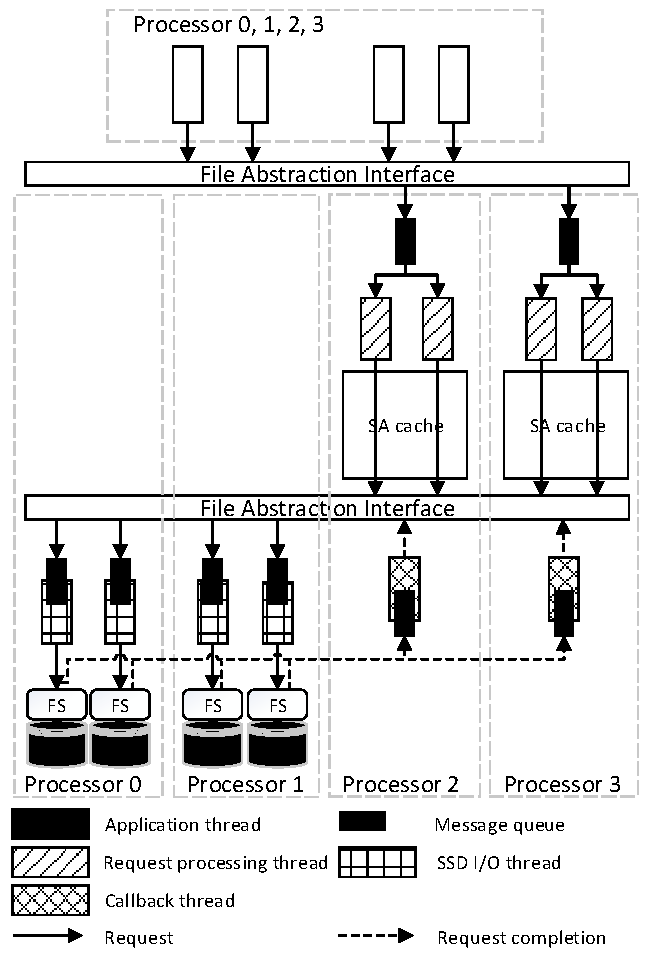
\includegraphics[scale=0.7]{figs/SAFS/NUMA-design.pdf}
\vspace{-5pt}
\caption{The architecture of the NUMA-SA cache on a four processor machine with 
two processors attached to SSDs. The page cache accesses SSDs with the same file
abstraction interface as the one used by applications and expose the file
abstraction interface to user applications.}
\label{numa_arch}
\vspace{-5pt}
\end{figure}

We extend the set-associative cache for the NUMA architectures
(NUMA-SA) to optimize for workloads with relatively high cache hit
rates and tackle hardware heterogeneity.
The NUMA-SA cache design was inspired by multicore operating systems that treat each 
core a node in a message-passing distributed system \cite{barrelfish}.  
However, we hybridize this concept with standard SMP programming models:  
we use message passing for inter-processor operations but use shared-memory among the 
cores within each processor.  Figure \ref{numa_arch} shows the design of NUMA-SA cache.
Each processor attached to SSDs has threads dedicated to performing I/O
for each SSD. The dedicated I/O thread removes contention for kernel and file locks.  
The processors without SSDs maintain page caches to serve applications I/O
requests.

I/O requests from applications are routed to the caching nodes through
message passing to reduce remote memory access. The caching nodes maintain
message passing queues and
a pool of threads for processing messages.
On completion of an I/O request, the data is written back to
the destination memory directly and then a reply is sent to the issuing thread.
This design opens opportunities to move application computation to the cache
to reduce remote memory access.

We separate I/O nodes from caching nodes in order to balance computation.
I/O operations require significant CPU and running a cache on an I/O node
overloads the processor and reduces IOPS.  This is a design decision, not a
requirement, i.e.~we can run a set-associative cache on the I/O nodes as well.
In a NUMA machine, a large fraction of I/Os require remote memory transfers.  
This happens when application threads run on other nodes than I/O nodes.
Separating the cache and I/O nodes does increase remote memory transfers.
However, balanced CPU utilization makes up for this effect in performance.
As systems scale to more processors, we expect that
few processors will have PCI buses, which will increase the CPU load on these nodes,
so that splitting these functions will continue to be advantageous.

Message passing creates many small requests and synchronizing these requests
can become expensive.
%Threads communicate with NUMA-SA cache by exchanging messages through
%a rendezvous message queue between them. 
Message passing may block sending
threads if their queue is full and receiving threads if their queue is empty.
Synchronization of requests often involves 
cache line invalidation on shared data and thread rescheduling. 
Frequent thread rescheduling wastes CPU cycles, preventing application threads 
from getting enough CPU.  
We reduce synchronization overheads by amortizing them over larger messages.

\section{Performance evaluation}
We evaluate our implementation with various workloads. We start with the
evaluation on the user-space file abstraction without caching to demonstrate
the raw performance of the hardware. We evaluate the page cache in the file
abstraction with various workloads from commercial data services and scientific
applications. We further integrate our system into the IOR benchmark \cite{IOR}
to measure its performance in a typical HPC environment.

We conduct experiments on a non-uniform memory architecture machine
with four Intel Xeon E5-4620 processors, clocked at 2.2GHz, and 512GB
memory of DDR3-1333. Each processor has eight cores with hyperthreading enabled, 
resulting in 16 logical cores. Only two processors in the machine have
PCI buses connected to them. The machine has three LSI
SAS 9217-8i host bus adapters (HBA) connected to a SuperMicro storage chassis, 
in which 16 OCZ Vertex 4  SSDs are installed. In addition to the LSI HBAs,
there is one RAID controller that connects to disks with root filesystem.
The machine runs Ubuntu Linux 12.04 and Linux kernel v3.2.30.

To compare the best performance of our system design with that of the Linux, 
we measure the system in two configurations: an SMP architecture
using a single processor and NUMA using all processors.  On all I/O measures,
Linux performs best from a single processor.  Remote memory operations make using
all four processors slower.  
\vspace{-10pt}
\begin{itemize}
\addtolength{\itemsep}{-5pt}
\item SMP configuration: 16 SSDs connect to one processor through
	two LSI HBAs controlling eight SSDs each. All threads run on the same processor.
	Data are striped across SSDs.
\item NUMA configuration: 16 SSDs are connected to two processors. Processor 0
  has five SSDs attached to an LSI HBA and one through the RAID controller.  
  Processor 1 has two LSI HBAs with five SSDs each. 
  Application threads are evenly distributed across all four processors.
	Data are distributed through a hash mapping that assigns 10\% more I/Os to the LSI HBA attached SSDs.
  The RAID controller is slower.
\end{itemize}
\vspace{-10pt}
Experiments use the configurations shown in Table
\ref{default_conf} if not stated otherwise.
\begin{table}
\begin{center}
\small
\begin{tabular}{|c|c|}
\hline
Linux I/O scheduler & noop \\
\hline
Page cache size & 512MB \\
\hline
Page eviction policy & GClock \\
\hline
Block size & 16 pages \\
\hline
Block mapping & striping (SMP)/hash (NUMA) \\
\hline
Page set size & 12 pages \\
\hline
AIO depth & 32 \\
\hline
Number of app threads & 16 \\
\hline
File system on SSDs & XFS \\
\hline
\end{tabular}
\normalsize
\end{center}
\caption{Default configuration of experiments.}
\label{default_conf}
\end{table}

\subsection{User-Space File Abstraction}
This section enumerates the effectiveness of the hardware and software
optimizations implemented in the SSD user-space file abstraction without caching,
showing the contribution of each. The size of the smallest
requests issued by the page cache is 4KB, so we focus on 4KB read and write
performance. In each experiment, we read/write 40GB data randomly through
the SSD file abstraction in 16 threads.

\begin{figure}[tb]
\begin{center}
\vspace{-15pt}
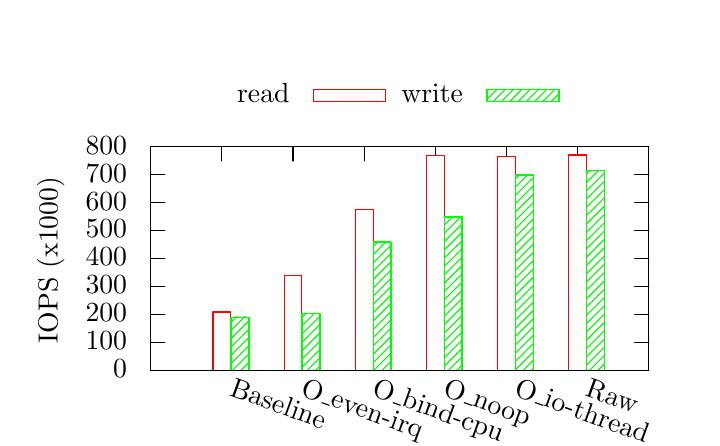
\begin{tikzpicture}[gnuplot]
%% generated with GNUPLOT 4.6p4 (Lua 5.1; terminal rev. 99, script rev. 100)
%% Wed 21 Oct 2015 09:55:31 PM EDT
\path (0.000,0.000) rectangle (8.382,4.826);
\gpcolor{color=gp lt color border}
\gpsetlinetype{gp lt border}
\gpsetlinewidth{1.00}
\draw[gp path] (1.504,1.000)--(1.684,1.000);
\draw[gp path] (7.829,1.000)--(7.649,1.000);
\node[gp node right] at (1.320,1.000) { 0};
\draw[gp path] (1.504,1.355)--(1.684,1.355);
\draw[gp path] (7.829,1.355)--(7.649,1.355);
\node[gp node right] at (1.320,1.355) { 100};
\draw[gp path] (1.504,1.710)--(1.684,1.710);
\draw[gp path] (7.829,1.710)--(7.649,1.710);
\node[gp node right] at (1.320,1.710) { 200};
\draw[gp path] (1.504,2.065)--(1.684,2.065);
\draw[gp path] (7.829,2.065)--(7.649,2.065);
\node[gp node right] at (1.320,2.065) { 300};
\draw[gp path] (1.504,2.421)--(1.684,2.421);
\draw[gp path] (7.829,2.421)--(7.649,2.421);
\node[gp node right] at (1.320,2.421) { 400};
\draw[gp path] (1.504,2.776)--(1.684,2.776);
\draw[gp path] (7.829,2.776)--(7.649,2.776);
\node[gp node right] at (1.320,2.776) { 500};
\draw[gp path] (1.504,3.131)--(1.684,3.131);
\draw[gp path] (7.829,3.131)--(7.649,3.131);
\node[gp node right] at (1.320,3.131) { 600};
\draw[gp path] (1.504,3.486)--(1.684,3.486);
\draw[gp path] (7.829,3.486)--(7.649,3.486);
\node[gp node right] at (1.320,3.486) { 700};
\draw[gp path] (1.504,3.841)--(1.684,3.841);
\draw[gp path] (7.829,3.841)--(7.649,3.841);
\node[gp node right] at (1.320,3.841) { 800};
\draw[gp path] (2.408,1.000)--(2.408,1.180);
\draw[gp path] (2.408,3.841)--(2.408,3.661);
\node[gp node left,rotate=-20] at (2.408,0.816) {Baseline};
\draw[gp path] (3.311,1.000)--(3.311,1.180);
\draw[gp path] (3.311,3.841)--(3.311,3.661);
\node[gp node left,rotate=-20] at (3.311,0.816) {O\_even-irq};
\draw[gp path] (4.215,1.000)--(4.215,1.180);
\draw[gp path] (4.215,3.841)--(4.215,3.661);
\node[gp node left,rotate=-20] at (4.215,0.816) {O\_bind-cpu};
\draw[gp path] (5.118,1.000)--(5.118,1.180);
\draw[gp path] (5.118,3.841)--(5.118,3.661);
\node[gp node left,rotate=-20] at (5.118,0.816) {O\_noop};
\draw[gp path] (6.022,1.000)--(6.022,1.180);
\draw[gp path] (6.022,3.841)--(6.022,3.661);
\node[gp node left,rotate=-20] at (6.022,0.816) {O\_io-thread};
\draw[gp path] (6.925,1.000)--(6.925,1.180);
\draw[gp path] (6.925,3.841)--(6.925,3.661);
\node[gp node left,rotate=-20] at (6.925,0.816) {Raw};
\draw[gp path] (1.504,3.841)--(1.504,1.000)--(7.829,1.000)--(7.829,3.841)--cycle;
\node[gp node center,rotate=-270] at (0.246,2.420) {IOPS (x1000)};
\node[gp node right] at (3.382,4.492) {read};
\def\gpfillpath{(3.566,4.415)--(4.482,4.415)--(4.482,4.569)--(3.566,4.569)--cycle}
\gpfill{color=gpbgfillcolor} \gpfillpath;
\gpfill{color=gp lt color 0,gp pattern 0,pattern color=.} \gpfillpath;
\gpcolor{color=gp lt color 0}
\gpsetlinetype{gp lt plot 0}
\draw[gp path] (3.566,4.415)--(4.482,4.415)--(4.482,4.569)--(3.566,4.569)--cycle;
\def\gpfillpath{(2.295,1.000)--(2.522,1.000)--(2.522,1.743)--(2.295,1.743)--cycle}
\gpfill{color=gpbgfillcolor} \gpfillpath;
\gpfill{color=gp lt color 0,gp pattern 0,pattern color=.} \gpfillpath;
\draw[gp path] (2.295,1.000)--(2.295,1.742)--(2.521,1.742)--(2.521,1.000)--cycle;
\def\gpfillpath{(3.198,1.000)--(3.425,1.000)--(3.425,2.204)--(3.198,2.204)--cycle}
\gpfill{color=gpbgfillcolor} \gpfillpath;
\gpfill{color=gp lt color 0,gp pattern 0,pattern color=.} \gpfillpath;
\draw[gp path] (3.198,1.000)--(3.198,2.203)--(3.424,2.203)--(3.424,1.000)--cycle;
\def\gpfillpath{(4.102,1.000)--(4.329,1.000)--(4.329,3.047)--(4.102,3.047)--cycle}
\gpfill{color=gpbgfillcolor} \gpfillpath;
\gpfill{color=gp lt color 0,gp pattern 0,pattern color=.} \gpfillpath;
\draw[gp path] (4.102,1.000)--(4.102,3.046)--(4.328,3.046)--(4.328,1.000)--cycle;
\def\gpfillpath{(5.005,1.000)--(5.232,1.000)--(5.232,3.727)--(5.005,3.727)--cycle}
\gpfill{color=gpbgfillcolor} \gpfillpath;
\gpfill{color=gp lt color 0,gp pattern 0,pattern color=.} \gpfillpath;
\draw[gp path] (5.005,1.000)--(5.005,3.726)--(5.231,3.726)--(5.231,1.000)--cycle;
\def\gpfillpath{(5.909,1.000)--(6.136,1.000)--(6.136,3.719)--(5.909,3.719)--cycle}
\gpfill{color=gpbgfillcolor} \gpfillpath;
\gpfill{color=gp lt color 0,gp pattern 0,pattern color=.} \gpfillpath;
\draw[gp path] (5.909,1.000)--(5.909,3.718)--(6.135,3.718)--(6.135,1.000)--cycle;
\def\gpfillpath{(6.812,1.000)--(7.039,1.000)--(7.039,3.737)--(6.812,3.737)--cycle}
\gpfill{color=gpbgfillcolor} \gpfillpath;
\gpfill{color=gp lt color 0,gp pattern 0,pattern color=.} \gpfillpath;
\draw[gp path] (6.812,1.000)--(6.812,3.736)--(7.038,3.736)--(7.038,1.000)--cycle;
\gpcolor{color=gp lt color border}
\node[gp node right] at (5.586,4.492) {write};
\def\gpfillpath{(5.770,4.415)--(6.686,4.415)--(6.686,4.569)--(5.770,4.569)--cycle}
\gpfill{color=gpbgfillcolor} \gpfillpath;
\gpfill{color=gp lt color 1,gp pattern 1,pattern color=.} \gpfillpath;
\gpcolor{color=gp lt color 1}
\gpsetlinetype{gp lt plot 1}
\draw[gp path] (5.770,4.415)--(6.686,4.415)--(6.686,4.569)--(5.770,4.569)--cycle;
\def\gpfillpath{(2.521,1.000)--(2.747,1.000)--(2.747,1.679)--(2.521,1.679)--cycle}
\gpfill{color=gpbgfillcolor} \gpfillpath;
\gpfill{color=gp lt color 1,gp pattern 1,pattern color=.} \gpfillpath;
\draw[gp path] (2.521,1.000)--(2.521,1.678)--(2.746,1.678)--(2.746,1.000)--cycle;
\def\gpfillpath{(3.424,1.000)--(3.651,1.000)--(3.651,1.729)--(3.424,1.729)--cycle}
\gpfill{color=gpbgfillcolor} \gpfillpath;
\gpfill{color=gp lt color 1,gp pattern 1,pattern color=.} \gpfillpath;
\draw[gp path] (3.424,1.000)--(3.424,1.728)--(3.650,1.728)--(3.650,1.000)--cycle;
\def\gpfillpath{(4.328,1.000)--(4.555,1.000)--(4.555,2.635)--(4.328,2.635)--cycle}
\gpfill{color=gpbgfillcolor} \gpfillpath;
\gpfill{color=gp lt color 1,gp pattern 1,pattern color=.} \gpfillpath;
\draw[gp path] (4.328,1.000)--(4.328,2.634)--(4.554,2.634)--(4.554,1.000)--cycle;
\def\gpfillpath{(5.231,1.000)--(5.458,1.000)--(5.458,2.951)--(5.231,2.951)--cycle}
\gpfill{color=gpbgfillcolor} \gpfillpath;
\gpfill{color=gp lt color 1,gp pattern 1,pattern color=.} \gpfillpath;
\draw[gp path] (5.231,1.000)--(5.231,2.950)--(5.457,2.950)--(5.457,1.000)--cycle;
\def\gpfillpath{(6.135,1.000)--(6.362,1.000)--(6.362,3.483)--(6.135,3.483)--cycle}
\gpfill{color=gpbgfillcolor} \gpfillpath;
\gpfill{color=gp lt color 1,gp pattern 1,pattern color=.} \gpfillpath;
\draw[gp path] (6.135,1.000)--(6.135,3.482)--(6.361,3.482)--(6.361,1.000)--cycle;
\def\gpfillpath{(7.038,1.000)--(7.265,1.000)--(7.265,3.542)--(7.038,3.542)--cycle}
\gpfill{color=gpbgfillcolor} \gpfillpath;
\gpfill{color=gp lt color 1,gp pattern 1,pattern color=.} \gpfillpath;
\draw[gp path] (7.038,1.000)--(7.038,3.541)--(7.264,3.541)--(7.264,1.000)--cycle;
\gpcolor{color=gp lt color border}
\gpsetlinetype{gp lt border}
\draw[gp path] (1.504,3.841)--(1.504,1.000)--(7.829,1.000)--(7.829,3.841)--cycle;
%% coordinates of the plot area
\gpdefrectangularnode{gp plot 1}{\pgfpoint{1.504cm}{1.000cm}}{\pgfpoint{7.829cm}{3.841cm}}
\end{tikzpicture}
%% gnuplot variables

\vspace{-15pt}
\caption{Optimizing page I/O on the SSD file abstraction accessed from
	an 8 core processor (SMP).
The bars show the aggregate IOPS when applying four optimizations successively
in comparison with the hardware's capabilities (raw).}
\label{ssd_impr}
\end{center}
\end{figure}

We perform four optimizations on the SSD file abstraction in succession
to optimize performance.
\vspace{-10pt}
\begin{itemize}
\addtolength{\itemsep}{-5pt}
\item {\bf O\_even-irq:} distribute interrupts evenly among all CPU cores;
\item {\bf O\_bind-cpu:} bind threads to the processor local to the SSD;
\item {\bf O\_noop:} use the noop I/O scheduler;
\item {\bf O\_io-thread:} create a dedicated I/O threads to access each SSD on behalf of
the application threads.
\end{itemize}
\vspace{-10pt}
Figure \ref{ssd_impr} shows I/O performance improvement of the SSD
file abstraction when applying these optimizations in succession.
%in the SMP configuration when threads run on the processor local to them.
%By applying the optimizations O1, O2, O3 and O4, we can improve the
Performance reaches a peak 765,000 read IOPS and 699,000 write IOPS from 
a single processor up from 209,000 and 191,000 IOPS unoptimized.
Distributing interrupts removes a CPU bottleneck for read.  Binding threads 
to the local processor has a profound impact, doubling both read and write by
eliminating remote operations.
Dedicated I/O threads improves write throughput, which we attribute to 
removing lock contention on the file system's inode.

When we apply all optimizations, the system realizes
the performance of raw SSD hardware, as shown in Figure \ref{ssd_impr}.
It only loses less than 1\% random read throughput
and 2.4\% random write throughput. The performance loss mainly comes from
disparity among SSDs, because the system performs at the speed
of the slowest SSD in the array.
When writing data to SSDs, individual SSDs slow down due to garbage
collection, which causes the entire SSD array to slow down. Therefore, write
performance loss is higher than read performance loss. 
These performance losses compare well with the 
10\% performance loss measured by Caulfield \cite{Caulfield10}.

When we apply all optimizations in the NUMA configuration, we approach the 
full potential of the hardware, reaching 1.23 million read IOPS.
We show performance alongside the
%With all optimizations, the performance of the SSD array in the NUMA configuration
the Fusion-IO ioDrive Octal \cite{fusion} for a comparison with state of the 
art memory-integrated NAND flash products (Table \ref{beat_fusion}). 
This reveals that our design realizes comparable
read performance using commodity hardware.
SSDs have a 4KB minimum block size so that 512 bytes write a partial block 
and, thus, slow.  The 766K 4KB writes offer a better point of comparison.

\begin{table}
\begin{center}
\small
\begin{tabular}{|c|c|c|c|c|}
\hline
& SSDFA & ioDrive Octal 5TB \\
\hline
Read IOPS (512B) & 1,228,100 & 1,190,000 \\
\hline
Write IOPS (512B) & 386,976 & 1,180,000 \\
\hline
Read IOPS (4KB) & 946,700 & N/A \\
\hline
Write IOPS (4KB) & 766,082 & N/A \\
\hline
Read Bandwidth (64 kB) & 6.8GB/s & 6.0 GB/s \\
\hline
Write Bandwidth (64 kB) & 5.6GB/s & 4.4 GB/s \\
\hline
\end{tabular}
\normalsize
\end{center}
\caption{The performance of NUMA SSD user-space file abstraction compared
with FusionIO ioDrive Octal.}
\label{beat_fusion}
\end{table}

\begin{figure}[tb]
\begin{center}
\vspace{-15pt}
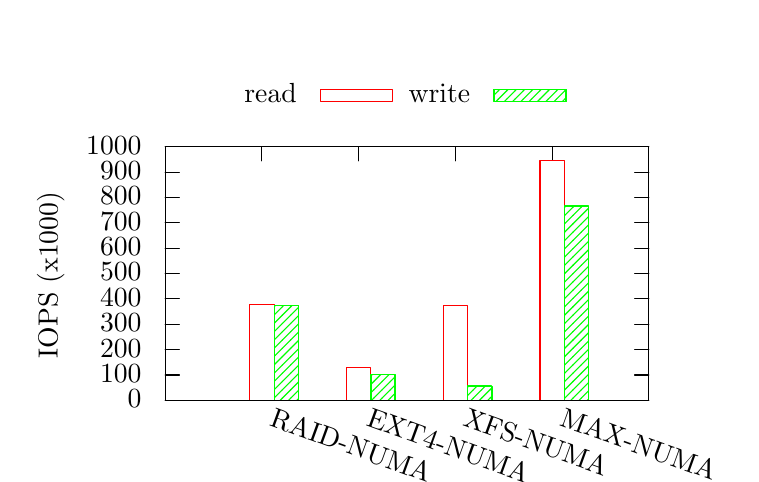
\begin{tikzpicture}[gnuplot]
%% generated with GNUPLOT 4.6p4 (Lua 5.1; terminal rev. 99, script rev. 100)
%% Wed 21 Oct 2015 09:59:22 PM EDT
\path (0.000,0.000) rectangle (8.382,5.080);
\gpcolor{color=gp lt color border}
\gpsetlinetype{gp lt border}
\gpsetlinewidth{1.00}
\draw[gp path] (1.688,0.874)--(1.868,0.874);
\draw[gp path] (7.829,0.874)--(7.649,0.874);
\node[gp node right] at (1.504,0.874) { 0};
\draw[gp path] (1.688,1.196)--(1.868,1.196);
\draw[gp path] (7.829,1.196)--(7.649,1.196);
\node[gp node right] at (1.504,1.196) { 100};
\draw[gp path] (1.688,1.518)--(1.868,1.518);
\draw[gp path] (7.829,1.518)--(7.649,1.518);
\node[gp node right] at (1.504,1.518) { 200};
\draw[gp path] (1.688,1.840)--(1.868,1.840);
\draw[gp path] (7.829,1.840)--(7.649,1.840);
\node[gp node right] at (1.504,1.840) { 300};
\draw[gp path] (1.688,2.162)--(1.868,2.162);
\draw[gp path] (7.829,2.162)--(7.649,2.162);
\node[gp node right] at (1.504,2.162) { 400};
\draw[gp path] (1.688,2.485)--(1.868,2.485);
\draw[gp path] (7.829,2.485)--(7.649,2.485);
\node[gp node right] at (1.504,2.485) { 500};
\draw[gp path] (1.688,2.807)--(1.868,2.807);
\draw[gp path] (7.829,2.807)--(7.649,2.807);
\node[gp node right] at (1.504,2.807) { 600};
\draw[gp path] (1.688,3.129)--(1.868,3.129);
\draw[gp path] (7.829,3.129)--(7.649,3.129);
\node[gp node right] at (1.504,3.129) { 700};
\draw[gp path] (1.688,3.451)--(1.868,3.451);
\draw[gp path] (7.829,3.451)--(7.649,3.451);
\node[gp node right] at (1.504,3.451) { 800};
\draw[gp path] (1.688,3.773)--(1.868,3.773);
\draw[gp path] (7.829,3.773)--(7.649,3.773);
\node[gp node right] at (1.504,3.773) { 900};
\draw[gp path] (1.688,4.095)--(1.868,4.095);
\draw[gp path] (7.829,4.095)--(7.649,4.095);
\node[gp node right] at (1.504,4.095) { 1000};
\draw[gp path] (2.916,0.874)--(2.916,1.054);
\draw[gp path] (2.916,4.095)--(2.916,3.915);
\node[gp node left,rotate=-20] at (2.916,0.690) {RAID-NUMA};
\draw[gp path] (4.144,0.874)--(4.144,1.054);
\draw[gp path] (4.144,4.095)--(4.144,3.915);
\node[gp node left,rotate=-20] at (4.144,0.690) {EXT4-NUMA};
\draw[gp path] (5.373,0.874)--(5.373,1.054);
\draw[gp path] (5.373,4.095)--(5.373,3.915);
\node[gp node left,rotate=-20] at (5.373,0.690) {XFS-NUMA};
\draw[gp path] (6.601,0.874)--(6.601,1.054);
\draw[gp path] (6.601,4.095)--(6.601,3.915);
\node[gp node left,rotate=-20] at (6.601,0.690) {MAX-NUMA};
\draw[gp path] (1.688,4.095)--(1.688,0.874)--(7.829,0.874)--(7.829,4.095)--cycle;
\node[gp node center,rotate=-270] at (0.246,2.484) {IOPS (x1000)};
\node[gp node right] at (3.474,4.746) {read};
\def\gpfillpath{(3.658,4.669)--(4.574,4.669)--(4.574,4.823)--(3.658,4.823)--cycle}
\gpfill{color=gpbgfillcolor} \gpfillpath;
\gpfill{color=gp lt color 0,gp pattern 0,pattern color=.} \gpfillpath;
\gpcolor{color=gp lt color 0}
\gpsetlinetype{gp lt plot 0}
\draw[gp path] (3.658,4.669)--(4.574,4.669)--(4.574,4.823)--(3.658,4.823)--cycle;
\def\gpfillpath{(2.763,0.874)--(3.071,0.874)--(3.071,2.091)--(2.763,2.091)--cycle}
\gpfill{color=gpbgfillcolor} \gpfillpath;
\gpfill{color=gp lt color 0,gp pattern 0,pattern color=.} \gpfillpath;
\draw[gp path] (2.763,0.874)--(2.763,2.090)--(3.070,2.090)--(3.070,0.874)--cycle;
\def\gpfillpath{(3.991,0.874)--(4.299,0.874)--(4.299,1.292)--(3.991,1.292)--cycle}
\gpfill{color=gpbgfillcolor} \gpfillpath;
\gpfill{color=gp lt color 0,gp pattern 0,pattern color=.} \gpfillpath;
\draw[gp path] (3.991,0.874)--(3.991,1.291)--(4.298,1.291)--(4.298,0.874)--cycle;
\def\gpfillpath{(5.219,0.874)--(5.527,0.874)--(5.527,2.085)--(5.219,2.085)--cycle}
\gpfill{color=gpbgfillcolor} \gpfillpath;
\gpfill{color=gp lt color 0,gp pattern 0,pattern color=.} \gpfillpath;
\draw[gp path] (5.219,0.874)--(5.219,2.084)--(5.526,2.084)--(5.526,0.874)--cycle;
\def\gpfillpath{(6.447,0.874)--(6.755,0.874)--(6.755,3.924)--(6.447,3.924)--cycle}
\gpfill{color=gpbgfillcolor} \gpfillpath;
\gpfill{color=gp lt color 0,gp pattern 0,pattern color=.} \gpfillpath;
\draw[gp path] (6.447,0.874)--(6.447,3.923)--(6.754,3.923)--(6.754,0.874)--cycle;
\gpcolor{color=gp lt color border}
\node[gp node right] at (5.678,4.746) {write};
\def\gpfillpath{(5.862,4.669)--(6.778,4.669)--(6.778,4.823)--(5.862,4.823)--cycle}
\gpfill{color=gpbgfillcolor} \gpfillpath;
\gpfill{color=gp lt color 1,gp pattern 1,pattern color=.} \gpfillpath;
\gpcolor{color=gp lt color 1}
\gpsetlinetype{gp lt plot 1}
\draw[gp path] (5.862,4.669)--(6.778,4.669)--(6.778,4.823)--(5.862,4.823)--cycle;
\def\gpfillpath{(3.070,0.874)--(3.378,0.874)--(3.378,2.081)--(3.070,2.081)--cycle}
\gpfill{color=gpbgfillcolor} \gpfillpath;
\gpfill{color=gp lt color 1,gp pattern 1,pattern color=.} \gpfillpath;
\draw[gp path] (3.070,0.874)--(3.070,2.080)--(3.377,2.080)--(3.377,0.874)--cycle;
\def\gpfillpath{(4.298,0.874)--(4.606,0.874)--(4.606,1.208)--(4.298,1.208)--cycle}
\gpfill{color=gpbgfillcolor} \gpfillpath;
\gpfill{color=gp lt color 1,gp pattern 1,pattern color=.} \gpfillpath;
\draw[gp path] (4.298,0.874)--(4.298,1.207)--(4.605,1.207)--(4.605,0.874)--cycle;
\def\gpfillpath{(5.526,0.874)--(5.834,0.874)--(5.834,1.058)--(5.526,1.058)--cycle}
\gpfill{color=gpbgfillcolor} \gpfillpath;
\gpfill{color=gp lt color 1,gp pattern 1,pattern color=.} \gpfillpath;
\draw[gp path] (5.526,0.874)--(5.526,1.057)--(5.833,1.057)--(5.833,0.874)--cycle;
\def\gpfillpath{(6.754,0.874)--(7.062,0.874)--(7.062,3.343)--(6.754,3.343)--cycle}
\gpfill{color=gpbgfillcolor} \gpfillpath;
\gpfill{color=gp lt color 1,gp pattern 1,pattern color=.} \gpfillpath;
\draw[gp path] (6.754,0.874)--(6.754,3.342)--(7.061,3.342)--(7.061,0.874)--cycle;
\gpcolor{color=gp lt color border}
\gpsetlinetype{gp lt border}
\draw[gp path] (1.688,4.095)--(1.688,0.874)--(7.829,0.874)--(7.829,4.095)--cycle;
%% coordinates of the plot area
\gpdefrectangularnode{gp plot 1}{\pgfpoint{1.688cm}{0.874cm}}{\pgfpoint{7.829cm}{4.095cm}}
\end{tikzpicture}
%% gnuplot variables

\vspace{-15pt}
\caption{Performance of our user-space file abstraction with Linux file systems
	and software RAID. All systems use optimizations O\_even-irq and O\_noop.}
\label{vs_soft_raid}
\end{center}
\end{figure}


We further compare our system with Linux software options, including 
block interfaces (software RAID) and file systems (Figure \ref{vs_soft_raid}).
Although software RAID can provide comparable performance in SMP configurations, 
NUMA results in a performance collapse to less than half the IOPS.   
Locking structures in file systems prevent scalable performance
on Linux software RAID.
%sothernd software RAID in the Linux kernel. Although
%software RAID can deliver the potential performance of the SSD array in the
%SMP configuration, none of the file system can perform well on the RAID.
Ext4 holds a lock to protect its data structure for both reads and writes.
Although XFS realizes good read performance, it performs poorly for writes
due to the exclusive locks that deschedule a thread if they are not
immediately available.
%has to use a heavier lock for writes. However, software RAID on the SSD
%array cannot perform well due to the problem of processor affinity. In summary,
%software RAID is not a right solution for an SSD array.

As an aside, we see a performance decrease in each SSD as more SSDs are
accessed in a HBA, as shown in Figure \ref{ssd_perf}. A single SSD can deliver
73,000 4KB-read IOPS and 61,000 4KB-write IOPS, while eight SSDs in a HBA
deliver only 47,000 read IOPS and 44,000 write IOPS per SSD.
Other work confirms this phenomena \cite{Foong10}. The aggregate IOPS
of an SSD array increases as the number of SSDs increases. Multiple HBAs scale.
%However,
%we did not observe similar performance degradation if each SSD is attached to
%a different HBA. This phenomenon is also confirmed by 
Performance degradation may be caused by lock contention in the HBA driver
as well as by the interfere inside the hardware itself. As a design rule, 
we attach as few SSDs to a HBA as possible to increase the overall I/O throughput of
the SSD array in the NUMA configuration.

\begin{figure}[tb]
\begin{center}
\vspace{-15pt}
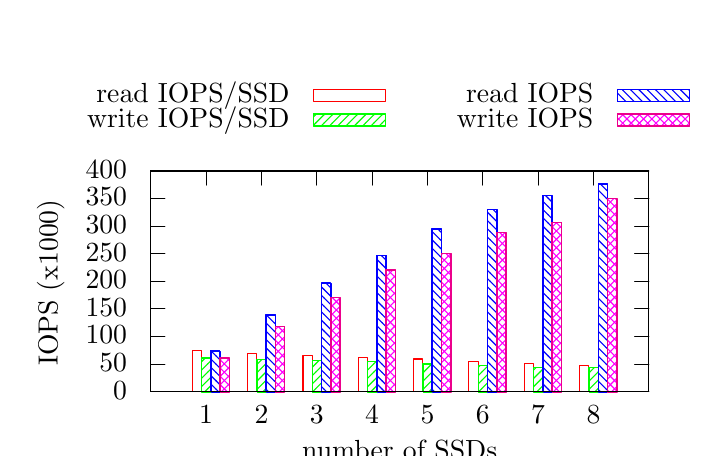
\begin{tikzpicture}[gnuplot]
%% generated with GNUPLOT 4.6p4 (Lua 5.1; terminal rev. 99, script rev. 100)
%% Wed 21 Oct 2015 09:55:50 PM EDT
\path (0.000,0.000) rectangle (8.382,5.080);
\gpcolor{color=gp lt color border}
\gpsetlinetype{gp lt border}
\gpsetlinewidth{1.00}
\draw[gp path] (1.504,0.985)--(1.684,0.985);
\draw[gp path] (7.829,0.985)--(7.649,0.985);
\node[gp node right] at (1.320,0.985) { 0};
\draw[gp path] (1.504,1.335)--(1.684,1.335);
\draw[gp path] (7.829,1.335)--(7.649,1.335);
\node[gp node right] at (1.320,1.335) { 50};
\draw[gp path] (1.504,1.686)--(1.684,1.686);
\draw[gp path] (7.829,1.686)--(7.649,1.686);
\node[gp node right] at (1.320,1.686) { 100};
\draw[gp path] (1.504,2.036)--(1.684,2.036);
\draw[gp path] (7.829,2.036)--(7.649,2.036);
\node[gp node right] at (1.320,2.036) { 150};
\draw[gp path] (1.504,2.386)--(1.684,2.386);
\draw[gp path] (7.829,2.386)--(7.649,2.386);
\node[gp node right] at (1.320,2.386) { 200};
\draw[gp path] (1.504,2.736)--(1.684,2.736);
\draw[gp path] (7.829,2.736)--(7.649,2.736);
\node[gp node right] at (1.320,2.736) { 250};
\draw[gp path] (1.504,3.087)--(1.684,3.087);
\draw[gp path] (7.829,3.087)--(7.649,3.087);
\node[gp node right] at (1.320,3.087) { 300};
\draw[gp path] (1.504,3.437)--(1.684,3.437);
\draw[gp path] (7.829,3.437)--(7.649,3.437);
\node[gp node right] at (1.320,3.437) { 350};
\draw[gp path] (1.504,3.787)--(1.684,3.787);
\draw[gp path] (7.829,3.787)--(7.649,3.787);
\node[gp node right] at (1.320,3.787) { 400};
\draw[gp path] (2.207,0.985)--(2.207,1.165);
\draw[gp path] (2.207,3.787)--(2.207,3.607);
\node[gp node center] at (2.207,0.677) {1};
\draw[gp path] (2.910,0.985)--(2.910,1.165);
\draw[gp path] (2.910,3.787)--(2.910,3.607);
\node[gp node center] at (2.910,0.677) {2};
\draw[gp path] (3.612,0.985)--(3.612,1.165);
\draw[gp path] (3.612,3.787)--(3.612,3.607);
\node[gp node center] at (3.612,0.677) {3};
\draw[gp path] (4.315,0.985)--(4.315,1.165);
\draw[gp path] (4.315,3.787)--(4.315,3.607);
\node[gp node center] at (4.315,0.677) {4};
\draw[gp path] (5.018,0.985)--(5.018,1.165);
\draw[gp path] (5.018,3.787)--(5.018,3.607);
\node[gp node center] at (5.018,0.677) {5};
\draw[gp path] (5.721,0.985)--(5.721,1.165);
\draw[gp path] (5.721,3.787)--(5.721,3.607);
\node[gp node center] at (5.721,0.677) {6};
\draw[gp path] (6.423,0.985)--(6.423,1.165);
\draw[gp path] (6.423,3.787)--(6.423,3.607);
\node[gp node center] at (6.423,0.677) {7};
\draw[gp path] (7.126,0.985)--(7.126,1.165);
\draw[gp path] (7.126,3.787)--(7.126,3.607);
\node[gp node center] at (7.126,0.677) {8};
\draw[gp path] (1.504,3.787)--(1.504,0.985)--(7.829,0.985)--(7.829,3.787)--cycle;
\node[gp node center,rotate=-270] at (0.246,2.386) {IOPS (x1000)};
\node[gp node center] at (4.666,0.215) {number of SSDs};
\node[gp node right] at (3.382,4.746) {read IOPS/SSD};
\def\gpfillpath{(3.566,4.669)--(4.482,4.669)--(4.482,4.823)--(3.566,4.823)--cycle}
\gpfill{color=gpbgfillcolor} \gpfillpath;
\gpfill{color=gp lt color 0,gp pattern 0,pattern color=.} \gpfillpath;
\gpcolor{color=gp lt color 0}
\gpsetlinetype{gp lt plot 0}
\draw[gp path] (3.566,4.669)--(4.482,4.669)--(4.482,4.823)--(3.566,4.823)--cycle;
\def\gpfillpath{(2.031,0.985)--(2.149,0.985)--(2.149,1.506)--(2.031,1.506)--cycle}
\gpfill{color=gpbgfillcolor} \gpfillpath;
\gpfill{color=gp lt color 0,gp pattern 0,pattern color=.} \gpfillpath;
\draw[gp path] (2.031,0.985)--(2.031,1.505)--(2.148,1.505)--(2.148,0.985)--cycle;
\def\gpfillpath{(2.734,0.985)--(2.852,0.985)--(2.852,1.474)--(2.734,1.474)--cycle}
\gpfill{color=gpbgfillcolor} \gpfillpath;
\gpfill{color=gp lt color 0,gp pattern 0,pattern color=.} \gpfillpath;
\draw[gp path] (2.734,0.985)--(2.734,1.473)--(2.851,1.473)--(2.851,0.985)--cycle;
\def\gpfillpath{(3.437,0.985)--(3.555,0.985)--(3.555,1.446)--(3.437,1.446)--cycle}
\gpfill{color=gpbgfillcolor} \gpfillpath;
\gpfill{color=gp lt color 0,gp pattern 0,pattern color=.} \gpfillpath;
\draw[gp path] (3.437,0.985)--(3.437,1.445)--(3.554,1.445)--(3.554,0.985)--cycle;
\def\gpfillpath{(4.139,0.985)--(4.258,0.985)--(4.258,1.418)--(4.139,1.418)--cycle}
\gpfill{color=gpbgfillcolor} \gpfillpath;
\gpfill{color=gp lt color 0,gp pattern 0,pattern color=.} \gpfillpath;
\draw[gp path] (4.139,0.985)--(4.139,1.417)--(4.257,1.417)--(4.257,0.985)--cycle;
\def\gpfillpath{(4.842,0.985)--(4.960,0.985)--(4.960,1.400)--(4.842,1.400)--cycle}
\gpfill{color=gpbgfillcolor} \gpfillpath;
\gpfill{color=gp lt color 0,gp pattern 0,pattern color=.} \gpfillpath;
\draw[gp path] (4.842,0.985)--(4.842,1.399)--(4.959,1.399)--(4.959,0.985)--cycle;
\def\gpfillpath{(5.545,0.985)--(5.663,0.985)--(5.663,1.372)--(5.545,1.372)--cycle}
\gpfill{color=gpbgfillcolor} \gpfillpath;
\gpfill{color=gp lt color 0,gp pattern 0,pattern color=.} \gpfillpath;
\draw[gp path] (5.545,0.985)--(5.545,1.371)--(5.662,1.371)--(5.662,0.985)--cycle;
\def\gpfillpath{(6.248,0.985)--(6.366,0.985)--(6.366,1.342)--(6.248,1.342)--cycle}
\gpfill{color=gpbgfillcolor} \gpfillpath;
\gpfill{color=gp lt color 0,gp pattern 0,pattern color=.} \gpfillpath;
\draw[gp path] (6.248,0.985)--(6.248,1.341)--(6.365,1.341)--(6.365,0.985)--cycle;
\def\gpfillpath{(6.951,0.985)--(7.069,0.985)--(7.069,1.316)--(6.951,1.316)--cycle}
\gpfill{color=gpbgfillcolor} \gpfillpath;
\gpfill{color=gp lt color 0,gp pattern 0,pattern color=.} \gpfillpath;
\draw[gp path] (6.951,0.985)--(6.951,1.315)--(7.068,1.315)--(7.068,0.985)--cycle;
\gpcolor{color=gp lt color border}
\node[gp node right] at (3.382,4.438) {write IOPS/SSD};
\def\gpfillpath{(3.566,4.361)--(4.482,4.361)--(4.482,4.515)--(3.566,4.515)--cycle}
\gpfill{color=gpbgfillcolor} \gpfillpath;
\gpfill{color=gp lt color 1,gp pattern 1,pattern color=.} \gpfillpath;
\gpcolor{color=gp lt color 1}
\gpsetlinetype{gp lt plot 1}
\draw[gp path] (3.566,4.361)--(4.482,4.361)--(4.482,4.515)--(3.566,4.515)--cycle;
\def\gpfillpath{(2.148,0.985)--(2.266,0.985)--(2.266,1.413)--(2.148,1.413)--cycle}
\gpfill{color=gpbgfillcolor} \gpfillpath;
\gpfill{color=gp lt color 1,gp pattern 1,pattern color=.} \gpfillpath;
\draw[gp path] (2.148,0.985)--(2.148,1.412)--(2.265,1.412)--(2.265,0.985)--cycle;
\def\gpfillpath{(2.851,0.985)--(2.969,0.985)--(2.969,1.399)--(2.851,1.399)--cycle}
\gpfill{color=gpbgfillcolor} \gpfillpath;
\gpfill{color=gp lt color 1,gp pattern 1,pattern color=.} \gpfillpath;
\draw[gp path] (2.851,0.985)--(2.851,1.398)--(2.968,1.398)--(2.968,0.985)--cycle;
\def\gpfillpath{(3.554,0.985)--(3.672,0.985)--(3.672,1.384)--(3.554,1.384)--cycle}
\gpfill{color=gpbgfillcolor} \gpfillpath;
\gpfill{color=gp lt color 1,gp pattern 1,pattern color=.} \gpfillpath;
\draw[gp path] (3.554,0.985)--(3.554,1.383)--(3.671,1.383)--(3.671,0.985)--cycle;
\def\gpfillpath{(4.257,0.985)--(4.375,0.985)--(4.375,1.373)--(4.257,1.373)--cycle}
\gpfill{color=gpbgfillcolor} \gpfillpath;
\gpfill{color=gp lt color 1,gp pattern 1,pattern color=.} \gpfillpath;
\draw[gp path] (4.257,0.985)--(4.257,1.372)--(4.374,1.372)--(4.374,0.985)--cycle;
\def\gpfillpath{(4.959,0.985)--(5.077,0.985)--(5.077,1.337)--(4.959,1.337)--cycle}
\gpfill{color=gpbgfillcolor} \gpfillpath;
\gpfill{color=gp lt color 1,gp pattern 1,pattern color=.} \gpfillpath;
\draw[gp path] (4.959,0.985)--(4.959,1.336)--(5.076,1.336)--(5.076,0.985)--cycle;
\def\gpfillpath{(5.662,0.985)--(5.780,0.985)--(5.780,1.323)--(5.662,1.323)--cycle}
\gpfill{color=gpbgfillcolor} \gpfillpath;
\gpfill{color=gp lt color 1,gp pattern 1,pattern color=.} \gpfillpath;
\draw[gp path] (5.662,0.985)--(5.662,1.322)--(5.779,1.322)--(5.779,0.985)--cycle;
\def\gpfillpath{(6.365,0.985)--(6.483,0.985)--(6.483,1.293)--(6.365,1.293)--cycle}
\gpfill{color=gpbgfillcolor} \gpfillpath;
\gpfill{color=gp lt color 1,gp pattern 1,pattern color=.} \gpfillpath;
\draw[gp path] (6.365,0.985)--(6.365,1.292)--(6.482,1.292)--(6.482,0.985)--cycle;
\def\gpfillpath{(7.068,0.985)--(7.186,0.985)--(7.186,1.292)--(7.068,1.292)--cycle}
\gpfill{color=gpbgfillcolor} \gpfillpath;
\gpfill{color=gp lt color 1,gp pattern 1,pattern color=.} \gpfillpath;
\draw[gp path] (7.068,0.985)--(7.068,1.291)--(7.185,1.291)--(7.185,0.985)--cycle;
\gpcolor{color=gp lt color border}
\node[gp node right] at (7.242,4.746) {read IOPS};
\def\gpfillpath{(7.426,4.669)--(8.342,4.669)--(8.342,4.823)--(7.426,4.823)--cycle}
\gpfill{color=gpbgfillcolor} \gpfillpath;
\gpfill{color=gp lt color 2,gp pattern 2,pattern color=.} \gpfillpath;
\gpcolor{color=gp lt color 2}
\gpsetlinetype{gp lt plot 2}
\draw[gp path] (7.426,4.669)--(8.342,4.669)--(8.342,4.823)--(7.426,4.823)--cycle;
\def\gpfillpath{(2.265,0.985)--(2.383,0.985)--(2.383,1.506)--(2.265,1.506)--cycle}
\gpfill{color=gpbgfillcolor} \gpfillpath;
\gpfill{color=gp lt color 2,gp pattern 2,pattern color=.} \gpfillpath;
\draw[gp path] (2.265,0.985)--(2.265,1.505)--(2.382,1.505)--(2.382,0.985)--cycle;
\def\gpfillpath{(2.968,0.985)--(3.086,0.985)--(3.086,1.961)--(2.968,1.961)--cycle}
\gpfill{color=gpbgfillcolor} \gpfillpath;
\gpfill{color=gp lt color 2,gp pattern 2,pattern color=.} \gpfillpath;
\draw[gp path] (2.968,0.985)--(2.968,1.960)--(3.085,1.960)--(3.085,0.985)--cycle;
\def\gpfillpath{(3.671,0.985)--(3.789,0.985)--(3.789,2.365)--(3.671,2.365)--cycle}
\gpfill{color=gpbgfillcolor} \gpfillpath;
\gpfill{color=gp lt color 2,gp pattern 2,pattern color=.} \gpfillpath;
\draw[gp path] (3.671,0.985)--(3.671,2.364)--(3.788,2.364)--(3.788,0.985)--cycle;
\def\gpfillpath{(4.374,0.985)--(4.492,0.985)--(4.492,2.714)--(4.374,2.714)--cycle}
\gpfill{color=gpbgfillcolor} \gpfillpath;
\gpfill{color=gp lt color 2,gp pattern 2,pattern color=.} \gpfillpath;
\draw[gp path] (4.374,0.985)--(4.374,2.713)--(4.491,2.713)--(4.491,0.985)--cycle;
\def\gpfillpath{(5.076,0.985)--(5.195,0.985)--(5.195,3.054)--(5.076,3.054)--cycle}
\gpfill{color=gpbgfillcolor} \gpfillpath;
\gpfill{color=gp lt color 2,gp pattern 2,pattern color=.} \gpfillpath;
\draw[gp path] (5.076,0.985)--(5.076,3.053)--(5.194,3.053)--(5.194,0.985)--cycle;
\def\gpfillpath{(5.779,0.985)--(5.897,0.985)--(5.897,3.300)--(5.779,3.300)--cycle}
\gpfill{color=gpbgfillcolor} \gpfillpath;
\gpfill{color=gp lt color 2,gp pattern 2,pattern color=.} \gpfillpath;
\draw[gp path] (5.779,0.985)--(5.779,3.299)--(5.896,3.299)--(5.896,0.985)--cycle;
\def\gpfillpath{(6.482,0.985)--(6.600,0.985)--(6.600,3.477)--(6.482,3.477)--cycle}
\gpfill{color=gpbgfillcolor} \gpfillpath;
\gpfill{color=gp lt color 2,gp pattern 2,pattern color=.} \gpfillpath;
\draw[gp path] (6.482,0.985)--(6.482,3.476)--(6.599,3.476)--(6.599,0.985)--cycle;
\def\gpfillpath{(7.185,0.985)--(7.303,0.985)--(7.303,3.625)--(7.185,3.625)--cycle}
\gpfill{color=gpbgfillcolor} \gpfillpath;
\gpfill{color=gp lt color 2,gp pattern 2,pattern color=.} \gpfillpath;
\draw[gp path] (7.185,0.985)--(7.185,3.624)--(7.302,3.624)--(7.302,0.985)--cycle;
\gpcolor{color=gp lt color border}
\node[gp node right] at (7.242,4.438) {write IOPS};
\def\gpfillpath{(7.426,4.361)--(8.342,4.361)--(8.342,4.515)--(7.426,4.515)--cycle}
\gpfill{color=gpbgfillcolor} \gpfillpath;
\gpfill{color=gp lt color 3,gp pattern 3,pattern color=.} \gpfillpath;
\gpcolor{color=gp lt color 3}
\gpsetlinetype{gp lt plot 3}
\draw[gp path] (7.426,4.361)--(8.342,4.361)--(8.342,4.515)--(7.426,4.515)--cycle;
\def\gpfillpath{(2.382,0.985)--(2.501,0.985)--(2.501,1.413)--(2.382,1.413)--cycle}
\gpfill{color=gpbgfillcolor} \gpfillpath;
\gpfill{color=gp lt color 3,gp pattern 3,pattern color=.} \gpfillpath;
\draw[gp path] (2.382,0.985)--(2.382,1.412)--(2.500,1.412)--(2.500,0.985)--cycle;
\def\gpfillpath{(3.085,0.985)--(3.203,0.985)--(3.203,1.812)--(3.085,1.812)--cycle}
\gpfill{color=gpbgfillcolor} \gpfillpath;
\gpfill{color=gp lt color 3,gp pattern 3,pattern color=.} \gpfillpath;
\draw[gp path] (3.085,0.985)--(3.085,1.811)--(3.202,1.811)--(3.202,0.985)--cycle;
\def\gpfillpath{(3.788,0.985)--(3.906,0.985)--(3.906,2.181)--(3.788,2.181)--cycle}
\gpfill{color=gpbgfillcolor} \gpfillpath;
\gpfill{color=gp lt color 3,gp pattern 3,pattern color=.} \gpfillpath;
\draw[gp path] (3.788,0.985)--(3.788,2.180)--(3.905,2.180)--(3.905,0.985)--cycle;
\def\gpfillpath{(4.491,0.985)--(4.609,0.985)--(4.609,2.534)--(4.491,2.534)--cycle}
\gpfill{color=gpbgfillcolor} \gpfillpath;
\gpfill{color=gp lt color 3,gp pattern 3,pattern color=.} \gpfillpath;
\draw[gp path] (4.491,0.985)--(4.491,2.533)--(4.608,2.533)--(4.608,0.985)--cycle;
\def\gpfillpath{(5.194,0.985)--(5.312,0.985)--(5.312,2.742)--(5.194,2.742)--cycle}
\gpfill{color=gpbgfillcolor} \gpfillpath;
\gpfill{color=gp lt color 3,gp pattern 3,pattern color=.} \gpfillpath;
\draw[gp path] (5.194,0.985)--(5.194,2.741)--(5.311,2.741)--(5.311,0.985)--cycle;
\def\gpfillpath{(5.896,0.985)--(6.014,0.985)--(6.014,3.009)--(5.896,3.009)--cycle}
\gpfill{color=gpbgfillcolor} \gpfillpath;
\gpfill{color=gp lt color 3,gp pattern 3,pattern color=.} \gpfillpath;
\draw[gp path] (5.896,0.985)--(5.896,3.008)--(6.013,3.008)--(6.013,0.985)--cycle;
\def\gpfillpath{(6.599,0.985)--(6.717,0.985)--(6.717,3.136)--(6.599,3.136)--cycle}
\gpfill{color=gpbgfillcolor} \gpfillpath;
\gpfill{color=gp lt color 3,gp pattern 3,pattern color=.} \gpfillpath;
\draw[gp path] (6.599,0.985)--(6.599,3.135)--(6.716,3.135)--(6.716,0.985)--cycle;
\def\gpfillpath{(7.302,0.985)--(7.420,0.985)--(7.420,3.438)--(7.302,3.438)--cycle}
\gpfill{color=gpbgfillcolor} \gpfillpath;
\gpfill{color=gp lt color 3,gp pattern 3,pattern color=.} \gpfillpath;
\draw[gp path] (7.302,0.985)--(7.302,3.437)--(7.419,3.437)--(7.419,0.985)--cycle;
\gpcolor{color=gp lt color border}
\gpsetlinetype{gp lt border}
\draw[gp path] (1.504,3.787)--(1.504,0.985)--(7.829,0.985)--(7.829,3.787)--cycle;
%% coordinates of the plot area
\gpdefrectangularnode{gp plot 1}{\pgfpoint{1.504cm}{0.985cm}}{\pgfpoint{7.829cm}{3.787cm}}
\end{tikzpicture}
%% gnuplot variables

\vspace{-15pt}
\caption{The 4KB read and write IOPS of individual SSDs and the aggregate IOPS
	of the SSD array with different numbers of SSDs in the array. All SSDs
	connect to a single HBA.}
\label{ssd_perf}
\end{center}
\end{figure}

\subsection{Set-Associative Caching}

We demonstrate the performance of set-associative and NUMA-SA caches under different
workloads to illustrate their overhead and scalability and compare
performance with the Linux page cache.

We choose workloads that exhibit high I/O rates and random access
that are representatives of cloud computing and data-intensive science.
We generated traces by running applications, capturing I/O system calls, and converting 
them into file accesses in the underlying data distribution.  System call traces 
ensure that I/O are not filtered by a cache.  Workloads include:

\vspace{-10pt}

\begin{itemize}
\addtolength{\itemsep}{-5pt}
\item Uniformly random: The workload samples 128 bytes from pages chosen
  randomly without replacement.  The workload generates no cache hits, 
%  we generate a random workload by accessing
%	one page at a time from a file of 40GB uniformly at random. Each time it
%	reads 128 bytes from a different page, so it generates no cache hits.
	accessing 10,485,760 unique pages with 10,485,760 physical reads.
\item Yahoo!~Cloud Serving Benchmark (YCSB) \cite{ycsb}:  We derived a 
  workload by inserting 30 million items into MemcacheDB 
  and performing 30 million lookups according to YCSB's read-only Zipfian workload.
	The workload has 39,188,480 reads from 5,748,822 pages. The size of each
	request is 4096 bytes.  
\item Neo4j \cite{neo4j}: This workload injects a LiveJournal social
	network \cite{livejournal} in Neo4j and searches for the shortest path
	between two random nodes with Dijkstra algorithm. 
 Neo4j sometimes scans multiple small objects on disks with separate reads, which biases 
 the cache hit rate.   We merge small sequential reads into
	a single read. With this change, the workload has 22,450,263 reads and
	113 writes from 1,086,955 pages. The request size varies from 1 bytes
	to 1,001,616 bytes. Most requests are small.  The mean request size
	is 57 bytes.
\item Synapse labelling: This workload was traces at the Open Connectome Project \url{openconnecto.me}
  and describes the output of a parallel computer-vision pipeline run on a 4 Teravoxel image volume of 
  mouse brain data.  The pipeline detects 19 million synapses (neural connections) that it writes to 
  spatial database.  Write throughput limits performance.  The workload labels 19,462,656 synapses in a 
  3-d array 
  using 16 parallel threads.  The workload has 19,462,656 unaligned writes of about 1000 bytes on average
  and updates 2,697,487 unique pages.
\end{itemize}
\vspace{-10pt}
For experiments with multiple application threads, we dynamically dispatch 
small batches of I/O using a shared work queue so that all threads finish at 
nearly the same time, regardless of system and workload heterogeneity.

We measure the performance of Linux page cache with careful optimizations.
We install Linux software RAID on the SSD array and install XFS on software
RAID. We run 256 threads to issue requests in parallel to
Linux page cache in order to provide sufficient I/O requests to the SSD array.
We disable read ahead to avoid the kernel to read unnecessary data.
Each thread opens the data file by itself because concurrent updates on a file handler
in a NUMA machine leads to expensive inter-processor cache line invalidation.
As shown in the previous section, XFS does not support parallel write, we only
measure read performance. 


\para{Random Workloads}

The first experiment demonstrates that set-associative caching relieves the processor
bottleneck on page replacement.
We run the uniform random workload with no cache hits and measure
IOPS and CPU utilization (Figure \ref{compare_cache}).
CPU cycles bound the IOPS of the Linux cache when run from a single processor---its best 
configuration.  Linux uses all cycles on all 8 CPU cores to achieves 641K IOPS.  The set-associative 
cache on the same hardware runs at under 80\% CPU utilization and increases IOPS by 20\%
to the maximal performance of the SSD hardware.
Running the same workload across the entire machine increases IOPS by 
another 20\% to almost 950K for NUMA-SA.  The same hardware configuration
for Linux results in an IOPS collapse.
Besides the poor performance of software RAID, a NUMA machine also amplifies
locking overhead on the Linux page cache. The severe lock contention
in the NUMA machine is caused by higher parallelism and
more expensive cache line invalidation.

\begin{figure}[tb]
\begin{center}
\vspace{-15pt}
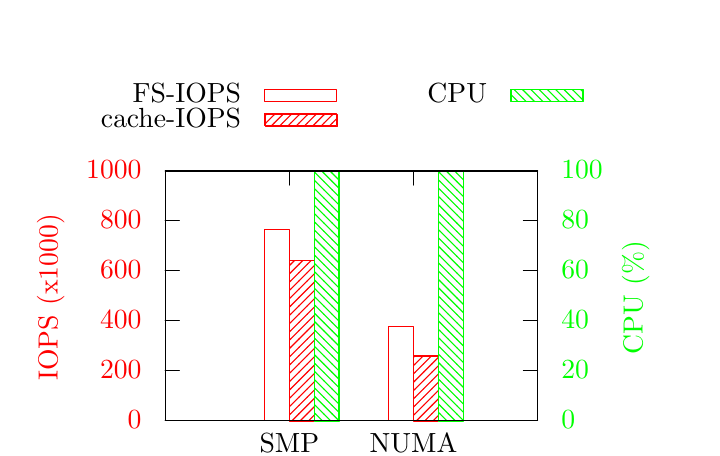
\begin{tikzpicture}[gnuplot]
%% generated with GNUPLOT 4.6p4 (Lua 5.1; terminal rev. 99, script rev. 100)
%% Wed 21 Oct 2015 10:00:04 PM EDT
\path (0.000,0.000) rectangle (8.382,5.080);
\gpcolor{color=gp lt color border}
\gpsetlinetype{gp lt border}
\gpsetlinewidth{1.00}
\draw[gp path] (1.688,0.616)--(1.868,0.616);
\gpcolor{color=gp lt color 0}
\node[gp node right] at (1.504,0.616) { 0};
\gpcolor{color=gp lt color border}
\draw[gp path] (1.688,1.250)--(1.868,1.250);
\gpcolor{color=gp lt color 0}
\node[gp node right] at (1.504,1.250) { 200};
\gpcolor{color=gp lt color border}
\draw[gp path] (1.688,1.884)--(1.868,1.884);
\gpcolor{color=gp lt color 0}
\node[gp node right] at (1.504,1.884) { 400};
\gpcolor{color=gp lt color border}
\draw[gp path] (1.688,2.519)--(1.868,2.519);
\gpcolor{color=gp lt color 0}
\node[gp node right] at (1.504,2.519) { 600};
\gpcolor{color=gp lt color border}
\draw[gp path] (1.688,3.153)--(1.868,3.153);
\gpcolor{color=gp lt color 0}
\node[gp node right] at (1.504,3.153) { 800};
\gpcolor{color=gp lt color border}
\draw[gp path] (1.688,3.787)--(1.868,3.787);
\gpcolor{color=gp lt color 0}
\node[gp node right] at (1.504,3.787) { 1000};
\gpcolor{color=gp lt color border}
\draw[gp path] (3.264,0.616)--(3.264,0.796);
\draw[gp path] (3.264,3.787)--(3.264,3.607);
\node[gp node center] at (3.264,0.308) {SMP};
\draw[gp path] (4.841,0.616)--(4.841,0.796);
\draw[gp path] (4.841,3.787)--(4.841,3.607);
\node[gp node center] at (4.841,0.308) {NUMA};
\draw[gp path] (6.417,0.616)--(6.237,0.616);
\gpcolor{color=gp lt color 1}
\node[gp node left] at (6.601,0.616) { 0};
\gpcolor{color=gp lt color border}
\draw[gp path] (6.417,1.250)--(6.237,1.250);
\gpcolor{color=gp lt color 1}
\node[gp node left] at (6.601,1.250) { 20};
\gpcolor{color=gp lt color border}
\draw[gp path] (6.417,1.884)--(6.237,1.884);
\gpcolor{color=gp lt color 1}
\node[gp node left] at (6.601,1.884) { 40};
\gpcolor{color=gp lt color border}
\draw[gp path] (6.417,2.519)--(6.237,2.519);
\gpcolor{color=gp lt color 1}
\node[gp node left] at (6.601,2.519) { 60};
\gpcolor{color=gp lt color border}
\draw[gp path] (6.417,3.153)--(6.237,3.153);
\gpcolor{color=gp lt color 1}
\node[gp node left] at (6.601,3.153) { 80};
\gpcolor{color=gp lt color border}
\draw[gp path] (6.417,3.787)--(6.237,3.787);
\gpcolor{color=gp lt color 1}
\node[gp node left] at (6.601,3.787) { 100};
\gpcolor{color=gp lt color border}
\draw[gp path] (1.688,3.787)--(1.688,0.616)--(6.417,0.616)--(6.417,3.787)--cycle;
\gpcolor{color=gp lt color 0}
\node[gp node center,rotate=-270] at (0.246,2.201) {IOPS (x1000)};
\gpcolor{color=gp lt color 1}
\node[gp node center,rotate=-270] at (7.674,2.201) {CPU (\%)};
\gpcolor{color=gp lt color border}
\node[gp node right] at (2.768,4.746) {FS-IOPS};
\def\gpfillpath{(2.952,4.669)--(3.868,4.669)--(3.868,4.823)--(2.952,4.823)--cycle}
\gpfill{color=gpbgfillcolor} \gpfillpath;
\gpfill{rgb color={1.000,0.000,0.000},gp pattern 0,pattern color=.} \gpfillpath;
\gpcolor{rgb color={1.000,0.000,0.000}}
\gpsetlinetype{gp lt plot 0}
\draw[gp path] (2.952,4.669)--(3.868,4.669)--(3.868,4.823)--(2.952,4.823)--cycle;
\def\gpfillpath{(2.949,0.616)--(3.265,0.616)--(3.265,3.049)--(2.949,3.049)--cycle}
\gpfill{color=gpbgfillcolor} \gpfillpath;
\gpfill{rgb color={1.000,0.000,0.000},gp pattern 0,pattern color=.} \gpfillpath;
\draw[gp path] (2.949,0.616)--(2.949,3.048)--(3.264,3.048)--(3.264,0.616)--cycle;
\def\gpfillpath{(4.525,0.616)--(4.842,0.616)--(4.842,1.808)--(4.525,1.808)--cycle}
\gpfill{color=gpbgfillcolor} \gpfillpath;
\gpfill{rgb color={1.000,0.000,0.000},gp pattern 0,pattern color=.} \gpfillpath;
\draw[gp path] (4.525,0.616)--(4.525,1.807)--(4.841,1.807)--(4.841,0.616)--cycle;
\gpcolor{color=gp lt color border}
\node[gp node right] at (2.768,4.438) {cache-IOPS};
\def\gpfillpath{(2.952,4.361)--(3.868,4.361)--(3.868,4.515)--(2.952,4.515)--cycle}
\gpfill{color=gpbgfillcolor} \gpfillpath;
\gpfill{rgb color={1.000,0.000,0.000},gp pattern 1,pattern color=.} \gpfillpath;
\gpcolor{rgb color={1.000,0.000,0.000}}
\gpsetlinetype{gp lt plot 1}
\draw[gp path] (2.952,4.361)--(3.868,4.361)--(3.868,4.515)--(2.952,4.515)--cycle;
\def\gpfillpath{(3.264,0.616)--(3.581,0.616)--(3.581,2.650)--(3.264,2.650)--cycle}
\gpfill{color=gpbgfillcolor} \gpfillpath;
\gpfill{rgb color={1.000,0.000,0.000},gp pattern 1,pattern color=.} \gpfillpath;
\draw[gp path] (3.264,0.616)--(3.264,2.649)--(3.580,2.649)--(3.580,0.616)--cycle;
\def\gpfillpath{(4.841,0.616)--(5.157,0.616)--(5.157,1.441)--(4.841,1.441)--cycle}
\gpfill{color=gpbgfillcolor} \gpfillpath;
\gpfill{rgb color={1.000,0.000,0.000},gp pattern 1,pattern color=.} \gpfillpath;
\draw[gp path] (4.841,0.616)--(4.841,1.440)--(5.156,1.440)--(5.156,0.616)--cycle;
\gpcolor{color=gp lt color border}
\node[gp node right] at (5.892,4.746) {CPU};
\def\gpfillpath{(6.076,4.669)--(6.992,4.669)--(6.992,4.823)--(6.076,4.823)--cycle}
\gpfill{color=gpbgfillcolor} \gpfillpath;
\gpfill{rgb color={0.000,1.000,0.000},gp pattern 2,pattern color=.} \gpfillpath;
\gpcolor{rgb color={0.000,1.000,0.000}}
\gpsetlinetype{gp lt plot 2}
\draw[gp path] (6.076,4.669)--(6.992,4.669)--(6.992,4.823)--(6.076,4.823)--cycle;
\def\gpfillpath{(3.580,0.616)--(3.896,0.616)--(3.896,3.788)--(3.580,3.788)--cycle}
\gpfill{color=gpbgfillcolor} \gpfillpath;
\gpfill{rgb color={0.000,1.000,0.000},gp pattern 2,pattern color=.} \gpfillpath;
\draw[gp path] (3.580,0.616)--(3.580,3.787)--(3.895,3.787)--(3.895,0.616)--cycle;
\def\gpfillpath{(5.156,0.616)--(5.472,0.616)--(5.472,3.788)--(5.156,3.788)--cycle}
\gpfill{color=gpbgfillcolor} \gpfillpath;
\gpfill{rgb color={0.000,1.000,0.000},gp pattern 2,pattern color=.} \gpfillpath;
\draw[gp path] (5.156,0.616)--(5.156,3.787)--(5.471,3.787)--(5.471,0.616)--cycle;
\gpcolor{color=gp lt color border}
\gpsetlinetype{gp lt border}
\draw[gp path] (1.688,3.787)--(1.688,0.616)--(6.417,0.616)--(6.417,3.787)--cycle;
%% coordinates of the plot area
\gpdefrectangularnode{gp plot 1}{\pgfpoint{1.688cm}{0.616cm}}{\pgfpoint{6.417cm}{3.787cm}}
\end{tikzpicture}
%% gnuplot variables

\vspace{-15pt}
\caption{IOPS and CPU for random read (0\% cache hit rate).}
\label{compare_cache}
\end{center}
\end{figure}

A comparison of IOPS as a function of cache hit rate
reveals that the set-associative caches outperform the Linux cache at high hit rates 
and that caching is necessary to realize application performance.
We measure IOPS under the uniform random workload for the Linux cache,
with set-associative caching, and without caching (SSDFA).
Overheads in the the Linux page cache make the set-associative cache 
realize roughly 30\% more IOPS than Linux at all cache hit rates (Figure \ref{SA_iops}(a)).  
The overheads come from different sources at different hit rates.  At 0\% the 
main overhead comes from I/O and cache replacement.  At 95\% the main overhead comes 
from the Linux virtual file system \cite{linux_vfs} and page lookup on the cache index.

Non-uniform memory widens the performance gap (Figure \ref{SA_iops}).
In this experiment application threads run on all processors.
NUMA-SA effectively avoids lock contention and reduces remote memory access,
but Linux page cache has severe lock contention in the NUMA machine.
This results in a factor of four improvement in user-perceived
IOPS when compared with the Linux cache.  Notably, the Linux cache does not match the 
performance of our SSD file abstraction (with no cachcing) until a 75\% 
cache hit rate, which reinforces the concept that lightweight I/O processing is 
equally important as caching to realize high IOPS.

%As shown in figure \ref{SA_iops}, SA-cache and NUMA-SA cache
%can perform well under all cache hit rates. 
The user-perceived I/O performance increases linearly with cache hit rates.
This is true for set-associative caching, NUMA-SA, and Linux.
The amount of CPU and effectiveness of the CPU dictates relative performance.
Linux is always CPU bound.

\begin{figure*}[tb]
\centering
\footnotesize
\vspace{-15pt}
\begin{subfigure}{.5\textwidth}
	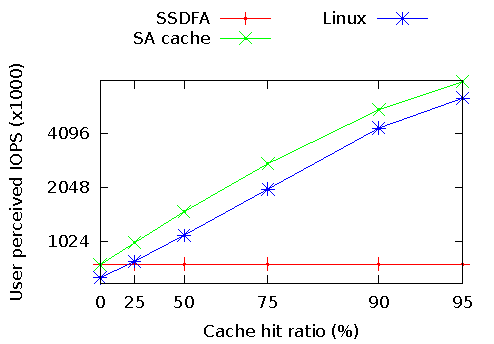
\includegraphics{figs/SAFS/new-SA-cache-hits.pdf}
	\label{sa_cache}
\vspace{-15pt}
\caption{SMP: one processor, eight applications cores.}
\end{subfigure}

%\vspace{-5pt}
\begin{subfigure}{.5\textwidth}
	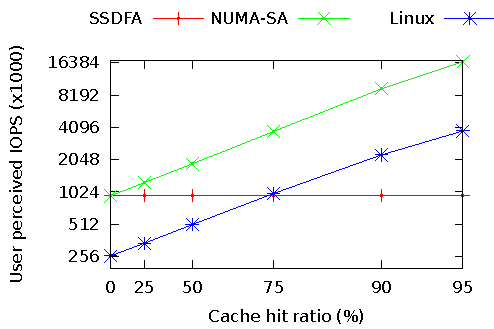
\includegraphics{figs/SAFS/new-NUMA-SA-hits.pdf}
	\label{numa_cache}
\vspace{-15pt}
\caption{NUMA: four processors, 32 application cores.}
\end{subfigure}
\caption{User-perceived IOPS as a function of cache hit rate.}
\label{SA_iops}
\end{figure*}


%\subsubsection{Impact of the page set size in SA-cache}
\para{The Impact of Page Set Size}

An important parameter in a set-associative cache is the size of a page set.
The parameter defines a tradeoff between cache hit rate and
CPU overhead within a page set.   Smaller pages sets reduce cache hit
rate and interference.  Larger page sets better approximate global caches, but 
increase contention and the overhead of page lookup and eviction.

The cache hit rates provide a lower bound on the page set size.
Figure \ref{hit_ratio} shows that the page set size has a limited impact on
the cache hit rate. 
Although a larger page set size increases the hit rate in all workloads, it
has more noticeable impact on the YCSB workload.  
Once the page set size increase beyond 12 pages per set, there are minimal 
benefits to cache hit rates.

We choose the smallest page set size that provides good cache hit rates 
across all workloads.  CPU overhead dictates small page sets.
CPU increases with page set size by up to 4.3\%.  Cache hit rates
result in better user-perceived performance by up to 3\%.
We choose 12 pages as the default configuration and use it for all subsequent experiments.

\begin{figure}[tb]
\begin{center}
\vspace{-15pt}
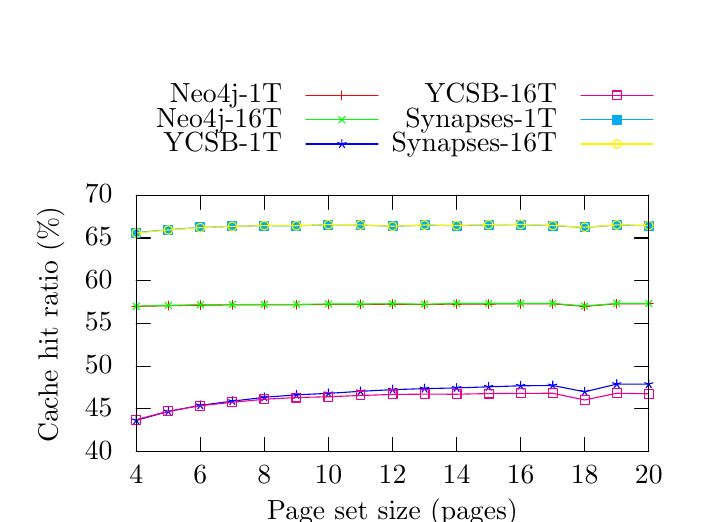
\begin{tikzpicture}[gnuplot]
%% generated with GNUPLOT 4.6p4 (Lua 5.1; terminal rev. 99, script rev. 100)
%% Wed 21 Oct 2015 09:53:58 PM EDT
\path (0.000,0.000) rectangle (8.382,5.842);
\gpcolor{color=gp lt color border}
\gpsetlinetype{gp lt border}
\gpsetlinewidth{1.00}
\draw[gp path] (1.320,0.985)--(1.500,0.985);
\draw[gp path] (7.829,0.985)--(7.649,0.985);
\node[gp node right] at (1.136,0.985) { 40};
\draw[gp path] (1.320,1.528)--(1.500,1.528);
\draw[gp path] (7.829,1.528)--(7.649,1.528);
\node[gp node right] at (1.136,1.528) { 45};
\draw[gp path] (1.320,2.070)--(1.500,2.070);
\draw[gp path] (7.829,2.070)--(7.649,2.070);
\node[gp node right] at (1.136,2.070) { 50};
\draw[gp path] (1.320,2.613)--(1.500,2.613);
\draw[gp path] (7.829,2.613)--(7.649,2.613);
\node[gp node right] at (1.136,2.613) { 55};
\draw[gp path] (1.320,3.156)--(1.500,3.156);
\draw[gp path] (7.829,3.156)--(7.649,3.156);
\node[gp node right] at (1.136,3.156) { 60};
\draw[gp path] (1.320,3.698)--(1.500,3.698);
\draw[gp path] (7.829,3.698)--(7.649,3.698);
\node[gp node right] at (1.136,3.698) { 65};
\draw[gp path] (1.320,4.241)--(1.500,4.241);
\draw[gp path] (7.829,4.241)--(7.649,4.241);
\node[gp node right] at (1.136,4.241) { 70};
\draw[gp path] (1.320,0.985)--(1.320,1.165);
\draw[gp path] (1.320,4.241)--(1.320,4.061);
\node[gp node center] at (1.320,0.677) { 4};
\draw[gp path] (2.134,0.985)--(2.134,1.165);
\draw[gp path] (2.134,4.241)--(2.134,4.061);
\node[gp node center] at (2.134,0.677) { 6};
\draw[gp path] (2.947,0.985)--(2.947,1.165);
\draw[gp path] (2.947,4.241)--(2.947,4.061);
\node[gp node center] at (2.947,0.677) { 8};
\draw[gp path] (3.761,0.985)--(3.761,1.165);
\draw[gp path] (3.761,4.241)--(3.761,4.061);
\node[gp node center] at (3.761,0.677) { 10};
\draw[gp path] (4.575,0.985)--(4.575,1.165);
\draw[gp path] (4.575,4.241)--(4.575,4.061);
\node[gp node center] at (4.575,0.677) { 12};
\draw[gp path] (5.388,0.985)--(5.388,1.165);
\draw[gp path] (5.388,4.241)--(5.388,4.061);
\node[gp node center] at (5.388,0.677) { 14};
\draw[gp path] (6.202,0.985)--(6.202,1.165);
\draw[gp path] (6.202,4.241)--(6.202,4.061);
\node[gp node center] at (6.202,0.677) { 16};
\draw[gp path] (7.015,0.985)--(7.015,1.165);
\draw[gp path] (7.015,4.241)--(7.015,4.061);
\node[gp node center] at (7.015,0.677) { 18};
\draw[gp path] (7.829,0.985)--(7.829,1.165);
\draw[gp path] (7.829,4.241)--(7.829,4.061);
\node[gp node center] at (7.829,0.677) { 20};
\draw[gp path] (1.320,4.241)--(1.320,0.985)--(7.829,0.985)--(7.829,4.241)--cycle;
\node[gp node center,rotate=-270] at (0.246,2.613) {Cache hit ratio (\%)};
\node[gp node center] at (4.574,0.215) {Page set size (pages)};
\node[gp node right] at (3.290,5.508) {Neo4j-1T};
\gpcolor{color=gp lt color 0}
\gpsetlinetype{gp lt plot 0}
\draw[gp path] (3.474,5.508)--(4.390,5.508);
\draw[gp path] (1.320,2.829)--(1.727,2.839)--(2.134,2.845)--(2.540,2.849)--(2.947,2.851)%
  --(3.354,2.850)--(3.761,2.855)--(4.168,2.855)--(4.575,2.858)--(4.981,2.853)--(5.388,2.860)%
  --(5.795,2.860)--(6.202,2.862)--(6.609,2.862)--(7.015,2.830)--(7.422,2.863)--(7.829,2.862);
\gpsetpointsize{4.00}
\gppoint{gp mark 1}{(1.320,2.829)}
\gppoint{gp mark 1}{(1.727,2.839)}
\gppoint{gp mark 1}{(2.134,2.845)}
\gppoint{gp mark 1}{(2.540,2.849)}
\gppoint{gp mark 1}{(2.947,2.851)}
\gppoint{gp mark 1}{(3.354,2.850)}
\gppoint{gp mark 1}{(3.761,2.855)}
\gppoint{gp mark 1}{(4.168,2.855)}
\gppoint{gp mark 1}{(4.575,2.858)}
\gppoint{gp mark 1}{(4.981,2.853)}
\gppoint{gp mark 1}{(5.388,2.860)}
\gppoint{gp mark 1}{(5.795,2.860)}
\gppoint{gp mark 1}{(6.202,2.862)}
\gppoint{gp mark 1}{(6.609,2.862)}
\gppoint{gp mark 1}{(7.015,2.830)}
\gppoint{gp mark 1}{(7.422,2.863)}
\gppoint{gp mark 1}{(7.829,2.862)}
\gppoint{gp mark 1}{(3.932,5.508)}
\gpcolor{color=gp lt color border}
\node[gp node right] at (3.290,5.200) {Neo4j-16T};
\gpcolor{color=gp lt color 1}
\gpsetlinetype{gp lt plot 1}
\draw[gp path] (3.474,5.200)--(4.390,5.200);
\draw[gp path] (1.320,2.831)--(1.727,2.842)--(2.134,2.850)--(2.540,2.852)--(2.947,2.855)%
  --(3.354,2.855)--(3.761,2.860)--(4.168,2.859)--(4.575,2.863)--(4.981,2.857)--(5.388,2.866)%
  --(5.795,2.866)--(6.202,2.867)--(6.609,2.867)--(7.015,2.834)--(7.422,2.867)--(7.829,2.867);
\gppoint{gp mark 2}{(1.320,2.831)}
\gppoint{gp mark 2}{(1.727,2.842)}
\gppoint{gp mark 2}{(2.134,2.850)}
\gppoint{gp mark 2}{(2.540,2.852)}
\gppoint{gp mark 2}{(2.947,2.855)}
\gppoint{gp mark 2}{(3.354,2.855)}
\gppoint{gp mark 2}{(3.761,2.860)}
\gppoint{gp mark 2}{(4.168,2.859)}
\gppoint{gp mark 2}{(4.575,2.863)}
\gppoint{gp mark 2}{(4.981,2.857)}
\gppoint{gp mark 2}{(5.388,2.866)}
\gppoint{gp mark 2}{(5.795,2.866)}
\gppoint{gp mark 2}{(6.202,2.867)}
\gppoint{gp mark 2}{(6.609,2.867)}
\gppoint{gp mark 2}{(7.015,2.834)}
\gppoint{gp mark 2}{(7.422,2.867)}
\gppoint{gp mark 2}{(7.829,2.867)}
\gppoint{gp mark 2}{(3.932,5.200)}
\gpcolor{color=gp lt color border}
\node[gp node right] at (3.290,4.892) {YCSB-1T};
\gpcolor{color=gp lt color 2}
\gpsetlinetype{gp lt plot 2}
\draw[gp path] (3.474,4.892)--(4.390,4.892);
\draw[gp path] (1.320,1.382)--(1.727,1.495)--(2.134,1.573)--(2.540,1.626)--(2.947,1.675)%
  --(3.354,1.706)--(3.761,1.725)--(4.168,1.751)--(4.575,1.772)--(4.981,1.785)--(5.388,1.794)%
  --(5.795,1.808)--(6.202,1.821)--(6.609,1.825)--(7.015,1.745)--(7.422,1.842)--(7.829,1.842);
\gppoint{gp mark 3}{(1.320,1.382)}
\gppoint{gp mark 3}{(1.727,1.495)}
\gppoint{gp mark 3}{(2.134,1.573)}
\gppoint{gp mark 3}{(2.540,1.626)}
\gppoint{gp mark 3}{(2.947,1.675)}
\gppoint{gp mark 3}{(3.354,1.706)}
\gppoint{gp mark 3}{(3.761,1.725)}
\gppoint{gp mark 3}{(4.168,1.751)}
\gppoint{gp mark 3}{(4.575,1.772)}
\gppoint{gp mark 3}{(4.981,1.785)}
\gppoint{gp mark 3}{(5.388,1.794)}
\gppoint{gp mark 3}{(5.795,1.808)}
\gppoint{gp mark 3}{(6.202,1.821)}
\gppoint{gp mark 3}{(6.609,1.825)}
\gppoint{gp mark 3}{(7.015,1.745)}
\gppoint{gp mark 3}{(7.422,1.842)}
\gppoint{gp mark 3}{(7.829,1.842)}
\gppoint{gp mark 3}{(3.932,4.892)}
\gpcolor{color=gp lt color border}
\node[gp node right] at (6.782,5.508) {YCSB-16T};
\gpcolor{color=gp lt color 3}
\gpsetlinetype{gp lt plot 3}
\draw[gp path] (6.966,5.508)--(7.882,5.508);
\draw[gp path] (1.320,1.391)--(1.727,1.498)--(2.134,1.568)--(2.540,1.611)--(2.947,1.650)%
  --(3.354,1.672)--(3.761,1.682)--(4.168,1.698)--(4.575,1.711)--(4.981,1.715)--(5.388,1.714)%
  --(5.795,1.722)--(6.202,1.725)--(6.609,1.726)--(7.015,1.641)--(7.422,1.726)--(7.829,1.720);
\gppoint{gp mark 4}{(1.320,1.391)}
\gppoint{gp mark 4}{(1.727,1.498)}
\gppoint{gp mark 4}{(2.134,1.568)}
\gppoint{gp mark 4}{(2.540,1.611)}
\gppoint{gp mark 4}{(2.947,1.650)}
\gppoint{gp mark 4}{(3.354,1.672)}
\gppoint{gp mark 4}{(3.761,1.682)}
\gppoint{gp mark 4}{(4.168,1.698)}
\gppoint{gp mark 4}{(4.575,1.711)}
\gppoint{gp mark 4}{(4.981,1.715)}
\gppoint{gp mark 4}{(5.388,1.714)}
\gppoint{gp mark 4}{(5.795,1.722)}
\gppoint{gp mark 4}{(6.202,1.725)}
\gppoint{gp mark 4}{(6.609,1.726)}
\gppoint{gp mark 4}{(7.015,1.641)}
\gppoint{gp mark 4}{(7.422,1.726)}
\gppoint{gp mark 4}{(7.829,1.720)}
\gppoint{gp mark 4}{(7.424,5.508)}
\gpcolor{color=gp lt color border}
\node[gp node right] at (6.782,5.200) {Synapses-1T};
\gpcolor{color=gp lt color 4}
\gpsetlinetype{gp lt plot 4}
\draw[gp path] (6.966,5.200)--(7.882,5.200);
\draw[gp path] (1.320,3.767)--(1.727,3.804)--(2.134,3.832)--(2.540,3.845)--(2.947,3.855)%
  --(3.354,3.852)--(3.761,3.867)--(4.168,3.863)--(4.575,3.846)--(4.981,3.861)--(5.388,3.855)%
  --(5.795,3.865)--(6.202,3.868)--(6.609,3.854)--(7.015,3.832)--(7.422,3.863)--(7.829,3.854);
\gppoint{gp mark 5}{(1.320,3.767)}
\gppoint{gp mark 5}{(1.727,3.804)}
\gppoint{gp mark 5}{(2.134,3.832)}
\gppoint{gp mark 5}{(2.540,3.845)}
\gppoint{gp mark 5}{(2.947,3.855)}
\gppoint{gp mark 5}{(3.354,3.852)}
\gppoint{gp mark 5}{(3.761,3.867)}
\gppoint{gp mark 5}{(4.168,3.863)}
\gppoint{gp mark 5}{(4.575,3.846)}
\gppoint{gp mark 5}{(4.981,3.861)}
\gppoint{gp mark 5}{(5.388,3.855)}
\gppoint{gp mark 5}{(5.795,3.865)}
\gppoint{gp mark 5}{(6.202,3.868)}
\gppoint{gp mark 5}{(6.609,3.854)}
\gppoint{gp mark 5}{(7.015,3.832)}
\gppoint{gp mark 5}{(7.422,3.863)}
\gppoint{gp mark 5}{(7.829,3.854)}
\gppoint{gp mark 5}{(7.424,5.200)}
\gpcolor{color=gp lt color border}
\node[gp node right] at (6.782,4.892) {Synapses-16T};
\gpcolor{color=gp lt color 5}
\gpsetlinetype{gp lt plot 5}
\draw[gp path] (6.966,4.892)--(7.882,4.892);
\draw[gp path] (1.320,3.761)--(1.727,3.800)--(2.134,3.829)--(2.540,3.845)--(2.947,3.856)%
  --(3.354,3.854)--(3.761,3.868)--(4.168,3.865)--(4.575,3.847)--(4.981,3.863)--(5.388,3.857)%
  --(5.795,3.868)--(6.202,3.871)--(6.609,3.857)--(7.015,3.835)--(7.422,3.865)--(7.829,3.857);
\gppoint{gp mark 6}{(1.320,3.761)}
\gppoint{gp mark 6}{(1.727,3.800)}
\gppoint{gp mark 6}{(2.134,3.829)}
\gppoint{gp mark 6}{(2.540,3.845)}
\gppoint{gp mark 6}{(2.947,3.856)}
\gppoint{gp mark 6}{(3.354,3.854)}
\gppoint{gp mark 6}{(3.761,3.868)}
\gppoint{gp mark 6}{(4.168,3.865)}
\gppoint{gp mark 6}{(4.575,3.847)}
\gppoint{gp mark 6}{(4.981,3.863)}
\gppoint{gp mark 6}{(5.388,3.857)}
\gppoint{gp mark 6}{(5.795,3.868)}
\gppoint{gp mark 6}{(6.202,3.871)}
\gppoint{gp mark 6}{(6.609,3.857)}
\gppoint{gp mark 6}{(7.015,3.835)}
\gppoint{gp mark 6}{(7.422,3.865)}
\gppoint{gp mark 6}{(7.829,3.857)}
\gppoint{gp mark 6}{(7.424,4.892)}
\gpcolor{color=gp lt color border}
\gpsetlinetype{gp lt border}
\draw[gp path] (1.320,4.241)--(1.320,0.985)--(7.829,0.985)--(7.829,4.241)--cycle;
%% coordinates of the plot area
\gpdefrectangularnode{gp plot 1}{\pgfpoint{1.320cm}{0.985cm}}{\pgfpoint{7.829cm}{4.241cm}}
\end{tikzpicture}
%% gnuplot variables

\vspace{-15pt}
\caption{The impact of page set sizes on cache hit rate in the set-associative cache
under real workloads both in one and 16 threads.}
\label{hit_ratio}
\end{center}
\end{figure}

%\subsubsection{Cache hit rates of SA-cache under real workloads}
\para{Cache Hit Rates}

We compare the cache hit rate of the set-associative cache with other page eviction
policies in order to quantify how well a cache with restricted associativity
emulates a global cache \cite{Sen02} on a variety of workloads.  
Figure \ref{cache_hits} compares the Clock-Pro page eviction
variant used by Linux \cite{clockpro}.
%as well as Belady's algorithm \cite{belady} to show optimal performance.
We also include the cache hit rate of GClock \cite{gclock} on a global
page buffer.   For the set-associative cache, we implement these replacement
policies on each page set as well as least-frequently used (LFU).
%All cache hit rates in Figure 
%\ref{cache_hits} are measured within a single thread. As we will show later,
%using more threads may cause more cache misses. 
When evaluating the cache
hit rate, we use the first half of a sequence of accesses to warm the cache
and the second half to evaluate the hit rate.

The set-associative has a cache hit rate comparable to a global page buffer.
It may lead to lower cache hit rate than a global page
buffer for the same page eviction policy, as shown in the YCSB case.
For workloads such as YCSB, which are 
dominated by frequency, LFU can generate more cache hits. It is difficult
to implement LFU in a global page buffer, but it is simple in the set-associative cache
due to the small size of a page set. We refer to \cite{hotstorage12} for
more detailed description of LFU implementation in the set-associative cache.

\begin{figure}[tb]
\begin{center}
\vspace{-15pt}
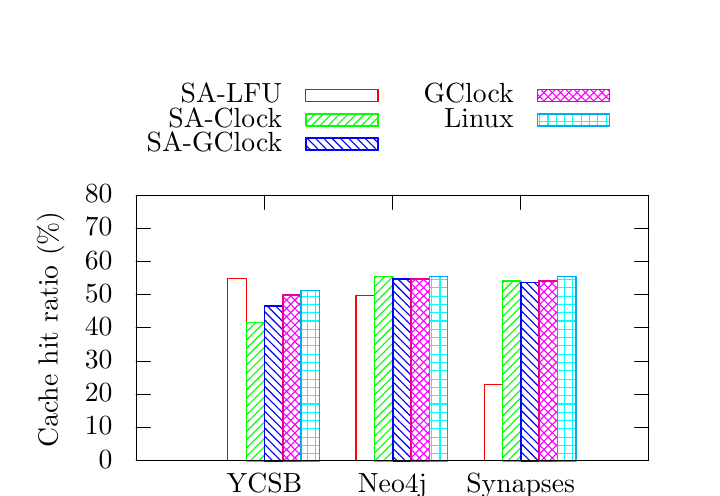
\begin{tikzpicture}[gnuplot]
%% generated with GNUPLOT 4.6p4 (Lua 5.1; terminal rev. 99, script rev. 100)
%% Wed 21 Oct 2015 09:53:32 PM EDT
\path (0.000,0.000) rectangle (8.382,5.588);
\gpcolor{color=gp lt color border}
\gpsetlinetype{gp lt border}
\gpsetlinewidth{1.00}
\draw[gp path] (1.320,0.616)--(1.500,0.616);
\draw[gp path] (7.829,0.616)--(7.649,0.616);
\node[gp node right] at (1.136,0.616) { 0};
\draw[gp path] (1.320,1.037)--(1.500,1.037);
\draw[gp path] (7.829,1.037)--(7.649,1.037);
\node[gp node right] at (1.136,1.037) { 10};
\draw[gp path] (1.320,1.459)--(1.500,1.459);
\draw[gp path] (7.829,1.459)--(7.649,1.459);
\node[gp node right] at (1.136,1.459) { 20};
\draw[gp path] (1.320,1.880)--(1.500,1.880);
\draw[gp path] (7.829,1.880)--(7.649,1.880);
\node[gp node right] at (1.136,1.880) { 30};
\draw[gp path] (1.320,2.302)--(1.500,2.302);
\draw[gp path] (7.829,2.302)--(7.649,2.302);
\node[gp node right] at (1.136,2.302) { 40};
\draw[gp path] (1.320,2.723)--(1.500,2.723);
\draw[gp path] (7.829,2.723)--(7.649,2.723);
\node[gp node right] at (1.136,2.723) { 50};
\draw[gp path] (1.320,3.144)--(1.500,3.144);
\draw[gp path] (7.829,3.144)--(7.649,3.144);
\node[gp node right] at (1.136,3.144) { 60};
\draw[gp path] (1.320,3.566)--(1.500,3.566);
\draw[gp path] (7.829,3.566)--(7.649,3.566);
\node[gp node right] at (1.136,3.566) { 70};
\draw[gp path] (1.320,3.987)--(1.500,3.987);
\draw[gp path] (7.829,3.987)--(7.649,3.987);
\node[gp node right] at (1.136,3.987) { 80};
\draw[gp path] (2.947,0.616)--(2.947,0.796);
\draw[gp path] (2.947,3.987)--(2.947,3.807);
\node[gp node center] at (2.947,0.308) {YCSB};
\draw[gp path] (4.575,0.616)--(4.575,0.796);
\draw[gp path] (4.575,3.987)--(4.575,3.807);
\node[gp node center] at (4.575,0.308) {Neo4j};
\draw[gp path] (6.202,0.616)--(6.202,0.796);
\draw[gp path] (6.202,3.987)--(6.202,3.807);
\node[gp node center] at (6.202,0.308) {Synapses};
\draw[gp path] (1.320,3.987)--(1.320,0.616)--(7.829,0.616)--(7.829,3.987)--cycle;
\node[gp node center,rotate=-270] at (0.246,2.301) {Cache hit ratio (\%)};
\node[gp node right] at (3.290,5.254) {SA-LFU};
\def\gpfillpath{(3.474,5.177)--(4.390,5.177)--(4.390,5.331)--(3.474,5.331)--cycle}
\gpfill{color=gpbgfillcolor} \gpfillpath;
\gpfill{color=gp lt color 0,gp pattern 0,pattern color=.} \gpfillpath;
\gpcolor{color=gp lt color 0}
\gpsetlinetype{gp lt plot 0}
\draw[gp path] (3.474,5.177)--(4.390,5.177)--(4.390,5.331)--(3.474,5.331)--cycle;
\def\gpfillpath{(2.482,0.616)--(2.716,0.616)--(2.716,2.928)--(2.482,2.928)--cycle}
\gpfill{color=gpbgfillcolor} \gpfillpath;
\gpfill{color=gp lt color 0,gp pattern 0,pattern color=.} \gpfillpath;
\draw[gp path] (2.482,0.616)--(2.482,2.927)--(2.715,2.927)--(2.715,0.616)--cycle;
\def\gpfillpath{(4.110,0.616)--(4.343,0.616)--(4.343,2.715)--(4.110,2.715)--cycle}
\gpfill{color=gpbgfillcolor} \gpfillpath;
\gpfill{color=gp lt color 0,gp pattern 0,pattern color=.} \gpfillpath;
\draw[gp path] (4.110,0.616)--(4.110,2.714)--(4.342,2.714)--(4.342,0.616)--cycle;
\def\gpfillpath{(5.737,0.616)--(5.970,0.616)--(5.970,1.590)--(5.737,1.590)--cycle}
\gpfill{color=gpbgfillcolor} \gpfillpath;
\gpfill{color=gp lt color 0,gp pattern 0,pattern color=.} \gpfillpath;
\draw[gp path] (5.737,0.616)--(5.737,1.589)--(5.969,1.589)--(5.969,0.616)--cycle;
\gpcolor{color=gp lt color border}
\node[gp node right] at (3.290,4.946) {SA-Clock};
\def\gpfillpath{(3.474,4.869)--(4.390,4.869)--(4.390,5.023)--(3.474,5.023)--cycle}
\gpfill{color=gpbgfillcolor} \gpfillpath;
\gpfill{color=gp lt color 1,gp pattern 1,pattern color=.} \gpfillpath;
\gpcolor{color=gp lt color 1}
\gpsetlinetype{gp lt plot 1}
\draw[gp path] (3.474,4.869)--(4.390,4.869)--(4.390,5.023)--(3.474,5.023)--cycle;
\def\gpfillpath{(2.715,0.616)--(2.948,0.616)--(2.948,2.374)--(2.715,2.374)--cycle}
\gpfill{color=gpbgfillcolor} \gpfillpath;
\gpfill{color=gp lt color 1,gp pattern 1,pattern color=.} \gpfillpath;
\draw[gp path] (2.715,0.616)--(2.715,2.373)--(2.947,2.373)--(2.947,0.616)--cycle;
\def\gpfillpath{(4.342,0.616)--(4.576,0.616)--(4.576,2.961)--(4.342,2.961)--cycle}
\gpfill{color=gpbgfillcolor} \gpfillpath;
\gpfill{color=gp lt color 1,gp pattern 1,pattern color=.} \gpfillpath;
\draw[gp path] (4.342,0.616)--(4.342,2.960)--(4.575,2.960)--(4.575,0.616)--cycle;
\def\gpfillpath{(5.969,0.616)--(6.203,0.616)--(6.203,2.903)--(5.969,2.903)--cycle}
\gpfill{color=gpbgfillcolor} \gpfillpath;
\gpfill{color=gp lt color 1,gp pattern 1,pattern color=.} \gpfillpath;
\draw[gp path] (5.969,0.616)--(5.969,2.902)--(6.202,2.902)--(6.202,0.616)--cycle;
\gpcolor{color=gp lt color border}
\node[gp node right] at (3.290,4.638) {SA-GClock};
\def\gpfillpath{(3.474,4.561)--(4.390,4.561)--(4.390,4.715)--(3.474,4.715)--cycle}
\gpfill{color=gpbgfillcolor} \gpfillpath;
\gpfill{color=gp lt color 2,gp pattern 2,pattern color=.} \gpfillpath;
\gpcolor{color=gp lt color 2}
\gpsetlinetype{gp lt plot 2}
\draw[gp path] (3.474,4.561)--(4.390,4.561)--(4.390,4.715)--(3.474,4.715)--cycle;
\def\gpfillpath{(2.947,0.616)--(3.181,0.616)--(3.181,2.585)--(2.947,2.585)--cycle}
\gpfill{color=gpbgfillcolor} \gpfillpath;
\gpfill{color=gp lt color 2,gp pattern 2,pattern color=.} \gpfillpath;
\draw[gp path] (2.947,0.616)--(2.947,2.584)--(3.180,2.584)--(3.180,0.616)--cycle;
\def\gpfillpath{(4.575,0.616)--(4.808,0.616)--(4.808,2.927)--(4.575,2.927)--cycle}
\gpfill{color=gpbgfillcolor} \gpfillpath;
\gpfill{color=gp lt color 2,gp pattern 2,pattern color=.} \gpfillpath;
\draw[gp path] (4.575,0.616)--(4.575,2.926)--(4.807,2.926)--(4.807,0.616)--cycle;
\def\gpfillpath{(6.202,0.616)--(6.435,0.616)--(6.435,2.882)--(6.202,2.882)--cycle}
\gpfill{color=gpbgfillcolor} \gpfillpath;
\gpfill{color=gp lt color 2,gp pattern 2,pattern color=.} \gpfillpath;
\draw[gp path] (6.202,0.616)--(6.202,2.881)--(6.434,2.881)--(6.434,0.616)--cycle;
\gpcolor{color=gp lt color border}
\node[gp node right] at (6.230,5.254) {GClock};
\def\gpfillpath{(6.414,5.177)--(7.330,5.177)--(7.330,5.331)--(6.414,5.331)--cycle}
\gpfill{color=gpbgfillcolor} \gpfillpath;
\gpfill{color=gp lt color 3,gp pattern 3,pattern color=.} \gpfillpath;
\gpcolor{color=gp lt color 3}
\gpsetlinetype{gp lt plot 3}
\draw[gp path] (6.414,5.177)--(7.330,5.177)--(7.330,5.331)--(6.414,5.331)--cycle;
\def\gpfillpath{(3.180,0.616)--(3.413,0.616)--(3.413,2.721)--(3.180,2.721)--cycle}
\gpfill{color=gpbgfillcolor} \gpfillpath;
\gpfill{color=gp lt color 3,gp pattern 3,pattern color=.} \gpfillpath;
\draw[gp path] (3.180,0.616)--(3.180,2.720)--(3.412,2.720)--(3.412,0.616)--cycle;
\def\gpfillpath{(4.807,0.616)--(5.040,0.616)--(5.040,2.927)--(4.807,2.927)--cycle}
\gpfill{color=gpbgfillcolor} \gpfillpath;
\gpfill{color=gp lt color 3,gp pattern 3,pattern color=.} \gpfillpath;
\draw[gp path] (4.807,0.616)--(4.807,2.926)--(5.039,2.926)--(5.039,0.616)--cycle;
\def\gpfillpath{(6.434,0.616)--(6.668,0.616)--(6.668,2.902)--(6.434,2.902)--cycle}
\gpfill{color=gpbgfillcolor} \gpfillpath;
\gpfill{color=gp lt color 3,gp pattern 3,pattern color=.} \gpfillpath;
\draw[gp path] (6.434,0.616)--(6.434,2.901)--(6.667,2.901)--(6.667,0.616)--cycle;
\gpcolor{color=gp lt color border}
\node[gp node right] at (6.230,4.946) {Linux};
\def\gpfillpath{(6.414,4.869)--(7.330,4.869)--(7.330,5.023)--(6.414,5.023)--cycle}
\gpfill{color=gpbgfillcolor} \gpfillpath;
\gpfill{color=gp lt color 4,gp pattern 4,pattern color=.} \gpfillpath;
\gpcolor{color=gp lt color 4}
\gpsetlinetype{gp lt plot 4}
\draw[gp path] (6.414,4.869)--(7.330,4.869)--(7.330,5.023)--(6.414,5.023)--cycle;
\def\gpfillpath{(3.412,0.616)--(3.646,0.616)--(3.646,2.780)--(3.412,2.780)--cycle}
\gpfill{color=gpbgfillcolor} \gpfillpath;
\gpfill{color=gp lt color 4,gp pattern 4,pattern color=.} \gpfillpath;
\draw[gp path] (3.412,0.616)--(3.412,2.779)--(3.645,2.779)--(3.645,0.616)--cycle;
\def\gpfillpath{(5.039,0.616)--(5.273,0.616)--(5.273,2.958)--(5.039,2.958)--cycle}
\gpfill{color=gpbgfillcolor} \gpfillpath;
\gpfill{color=gp lt color 4,gp pattern 4,pattern color=.} \gpfillpath;
\draw[gp path] (5.039,0.616)--(5.039,2.957)--(5.272,2.957)--(5.272,0.616)--cycle;
\def\gpfillpath{(6.667,0.616)--(6.900,0.616)--(6.900,2.956)--(6.667,2.956)--cycle}
\gpfill{color=gpbgfillcolor} \gpfillpath;
\gpfill{color=gp lt color 4,gp pattern 4,pattern color=.} \gpfillpath;
\draw[gp path] (6.667,0.616)--(6.667,2.955)--(6.899,2.955)--(6.899,0.616)--cycle;
\gpcolor{color=gp lt color border}
\gpsetlinetype{gp lt border}
\draw[gp path] (1.320,3.987)--(1.320,0.616)--(7.829,0.616)--(7.829,3.987)--cycle;
%% coordinates of the plot area
\gpdefrectangularnode{gp plot 1}{\pgfpoint{1.320cm}{0.616cm}}{\pgfpoint{7.829cm}{3.987cm}}
\end{tikzpicture}
%% gnuplot variables

\vspace{-15pt}
\caption{The cache hit rate of different cache designs under different workloads.}
\label{cache_hits}
\end{center}
\end{figure}

%\subsubsection{The performance of SA-cache under real workloads}
\para{Performance on Real Workloads}

For user-perceived performance, the increased IOPS  from hardware overwhelms any 
losses from decreased cache hit rates.   Figure \ref{real_workloads} shows 
the performance of set-associative and NUMA-SA caches in comparison to Linux's best 
performance under the Neo4j, YCSB, and Synapse workloads,
%All workloads do not access a large dataset, so the cache size is set to 512MB.
%We run SA-cache both in the SMP and NUMA configuration. As shown in figure
%\ref{SA_iops}, 
Again, the Linux page cache performs best on a single processor.
%than in the NUMA machine, so we only show its performance on a single processor.
%We cannot specify the size of Linux page cache. In order to measure
%the performance of Linux page cache, we fill memory until the size of Linux page
%cache is roughly 512MB.

The set-associative cache performs much better than Linux page cache under real workloads.
The Linux page cache achieves around 50--60\% of the maximal performance
for read-only workloads (Neo4j and YCSB).  Furthermore,  it 
delivers only 8,000 IOPS for an unaligned-write workload (Synapses). 
The poor performance of Linux page cache results from the exclusive locking in XFS, 
which only allows one thread to access the page cache and issue one request at a time to
the block devices. 
%Furthermore, unaligned writes cause the Linux page cache to read
%corresponding pages from the block devices, so that other threads have to wait
%for the read to be completed before preceeding.

\begin{figure}[tb]
\begin{center}
\vspace{-15pt}
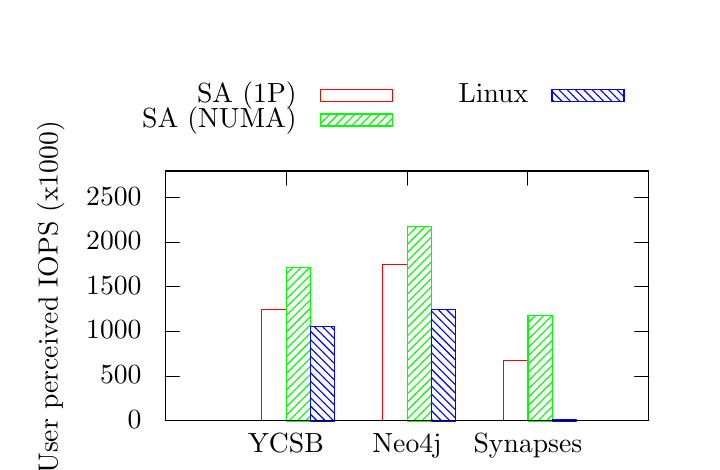
\begin{tikzpicture}[gnuplot]
%% generated with GNUPLOT 4.6p4 (Lua 5.1; terminal rev. 99, script rev. 100)
%% Wed 21 Oct 2015 09:55:15 PM EDT
\path (0.000,0.000) rectangle (8.382,5.080);
\gpcolor{color=gp lt color border}
\gpsetlinetype{gp lt border}
\gpsetlinewidth{1.00}
\draw[gp path] (1.688,0.616)--(1.868,0.616);
\draw[gp path] (7.829,0.616)--(7.649,0.616);
\node[gp node right] at (1.504,0.616) { 0};
\draw[gp path] (1.688,1.182)--(1.868,1.182);
\draw[gp path] (7.829,1.182)--(7.649,1.182);
\node[gp node right] at (1.504,1.182) { 500};
\draw[gp path] (1.688,1.749)--(1.868,1.749);
\draw[gp path] (7.829,1.749)--(7.649,1.749);
\node[gp node right] at (1.504,1.749) { 1000};
\draw[gp path] (1.688,2.315)--(1.868,2.315);
\draw[gp path] (7.829,2.315)--(7.649,2.315);
\node[gp node right] at (1.504,2.315) { 1500};
\draw[gp path] (1.688,2.881)--(1.868,2.881);
\draw[gp path] (7.829,2.881)--(7.649,2.881);
\node[gp node right] at (1.504,2.881) { 2000};
\draw[gp path] (1.688,3.447)--(1.868,3.447);
\draw[gp path] (7.829,3.447)--(7.649,3.447);
\node[gp node right] at (1.504,3.447) { 2500};
\draw[gp path] (3.223,0.616)--(3.223,0.796);
\draw[gp path] (3.223,3.787)--(3.223,3.607);
\node[gp node center] at (3.223,0.308) {YCSB};
\draw[gp path] (4.759,0.616)--(4.759,0.796);
\draw[gp path] (4.759,3.787)--(4.759,3.607);
\node[gp node center] at (4.759,0.308) {Neo4j};
\draw[gp path] (6.294,0.616)--(6.294,0.796);
\draw[gp path] (6.294,3.787)--(6.294,3.607);
\node[gp node center] at (6.294,0.308) {Synapses};
\draw[gp path] (1.688,3.787)--(1.688,0.616)--(7.829,0.616)--(7.829,3.787)--cycle;
\node[gp node center,rotate=-270] at (0.246,2.201) {User perceived IOPS (x1000)};
\node[gp node right] at (3.474,4.746) {SA (1P)};
\def\gpfillpath{(3.658,4.669)--(4.574,4.669)--(4.574,4.823)--(3.658,4.823)--cycle}
\gpfill{color=gpbgfillcolor} \gpfillpath;
\gpfill{color=gp lt color 0,gp pattern 0,pattern color=.} \gpfillpath;
\gpcolor{color=gp lt color 0}
\gpsetlinetype{gp lt plot 0}
\draw[gp path] (3.658,4.669)--(4.574,4.669)--(4.574,4.823)--(3.658,4.823)--cycle;
\def\gpfillpath{(2.916,0.616)--(3.224,0.616)--(3.224,2.027)--(2.916,2.027)--cycle}
\gpfill{color=gpbgfillcolor} \gpfillpath;
\gpfill{color=gp lt color 0,gp pattern 0,pattern color=.} \gpfillpath;
\draw[gp path] (2.916,0.616)--(2.916,2.026)--(3.223,2.026)--(3.223,0.616)--cycle;
\def\gpfillpath{(4.451,0.616)--(4.760,0.616)--(4.760,2.606)--(4.451,2.606)--cycle}
\gpfill{color=gpbgfillcolor} \gpfillpath;
\gpfill{color=gp lt color 0,gp pattern 0,pattern color=.} \gpfillpath;
\draw[gp path] (4.451,0.616)--(4.451,2.605)--(4.759,2.605)--(4.759,0.616)--cycle;
\def\gpfillpath{(5.987,0.616)--(6.295,0.616)--(6.295,1.377)--(5.987,1.377)--cycle}
\gpfill{color=gpbgfillcolor} \gpfillpath;
\gpfill{color=gp lt color 0,gp pattern 0,pattern color=.} \gpfillpath;
\draw[gp path] (5.987,0.616)--(5.987,1.376)--(6.294,1.376)--(6.294,0.616)--cycle;
\gpcolor{color=gp lt color border}
\node[gp node right] at (3.474,4.438) {SA (NUMA)};
\def\gpfillpath{(3.658,4.361)--(4.574,4.361)--(4.574,4.515)--(3.658,4.515)--cycle}
\gpfill{color=gpbgfillcolor} \gpfillpath;
\gpfill{color=gp lt color 1,gp pattern 1,pattern color=.} \gpfillpath;
\gpcolor{color=gp lt color 1}
\gpsetlinetype{gp lt plot 1}
\draw[gp path] (3.658,4.361)--(4.574,4.361)--(4.574,4.515)--(3.658,4.515)--cycle;
\def\gpfillpath{(3.223,0.616)--(3.531,0.616)--(3.531,2.564)--(3.223,2.564)--cycle}
\gpfill{color=gpbgfillcolor} \gpfillpath;
\gpfill{color=gp lt color 1,gp pattern 1,pattern color=.} \gpfillpath;
\draw[gp path] (3.223,0.616)--(3.223,2.563)--(3.530,2.563)--(3.530,0.616)--cycle;
\def\gpfillpath{(4.759,0.616)--(5.067,0.616)--(5.067,3.085)--(4.759,3.085)--cycle}
\gpfill{color=gpbgfillcolor} \gpfillpath;
\gpfill{color=gp lt color 1,gp pattern 1,pattern color=.} \gpfillpath;
\draw[gp path] (4.759,0.616)--(4.759,3.084)--(5.066,3.084)--(5.066,0.616)--cycle;
\def\gpfillpath{(6.294,0.616)--(6.602,0.616)--(6.602,1.955)--(6.294,1.955)--cycle}
\gpfill{color=gpbgfillcolor} \gpfillpath;
\gpfill{color=gp lt color 1,gp pattern 1,pattern color=.} \gpfillpath;
\draw[gp path] (6.294,0.616)--(6.294,1.954)--(6.601,1.954)--(6.601,0.616)--cycle;
\gpcolor{color=gp lt color border}
\node[gp node right] at (6.414,4.746) {Linux};
\def\gpfillpath{(6.598,4.669)--(7.514,4.669)--(7.514,4.823)--(6.598,4.823)--cycle}
\gpfill{color=gpbgfillcolor} \gpfillpath;
\gpfill{color=gp lt color 2,gp pattern 2,pattern color=.} \gpfillpath;
\gpcolor{color=gp lt color 2}
\gpsetlinetype{gp lt plot 2}
\draw[gp path] (6.598,4.669)--(7.514,4.669)--(7.514,4.823)--(6.598,4.823)--cycle;
\def\gpfillpath{(3.530,0.616)--(3.838,0.616)--(3.838,1.816)--(3.530,1.816)--cycle}
\gpfill{color=gpbgfillcolor} \gpfillpath;
\gpfill{color=gp lt color 2,gp pattern 2,pattern color=.} \gpfillpath;
\draw[gp path] (3.530,0.616)--(3.530,1.815)--(3.837,1.815)--(3.837,0.616)--cycle;
\def\gpfillpath{(5.066,0.616)--(5.374,0.616)--(5.374,2.029)--(5.066,2.029)--cycle}
\gpfill{color=gpbgfillcolor} \gpfillpath;
\gpfill{color=gp lt color 2,gp pattern 2,pattern color=.} \gpfillpath;
\draw[gp path] (5.066,0.616)--(5.066,2.028)--(5.373,2.028)--(5.373,0.616)--cycle;
\def\gpfillpath{(6.601,0.616)--(6.909,0.616)--(6.909,0.627)--(6.601,0.627)--cycle}
\gpfill{color=gpbgfillcolor} \gpfillpath;
\gpfill{color=gp lt color 2,gp pattern 2,pattern color=.} \gpfillpath;
\draw[gp path] (6.601,0.616)--(6.601,0.626)--(6.908,0.626)--(6.908,0.616)--cycle;
\gpcolor{color=gp lt color border}
\gpsetlinetype{gp lt border}
\draw[gp path] (1.688,3.787)--(1.688,0.616)--(7.829,0.616)--(7.829,3.787)--cycle;
%% coordinates of the plot area
\gpdefrectangularnode{gp plot 1}{\pgfpoint{1.688cm}{0.616cm}}{\pgfpoint{7.829cm}{3.787cm}}
\end{tikzpicture}
%% gnuplot variables

\vspace{-15pt}
\caption{The performance of the set-associative cache on real workloads}
\label{real_workloads}
\end{center}
\end{figure}

\subsection{HPC benchmark}

This section evaluates the overall performance of the user-space file
abstraction under HPC benchmarks. The typical setup of some HPC benchmarks
such as MADbench2 \cite{madbench2} has very large read/writes (in the
order of magnitude of 100 MB). However, our system is optimized mainly
for small random I/O accesses and requires many parallel I/O requests to
achieve maximal performance. We choose the IOR benchmark \cite{IOR} for
its flexibility.
IOR is a highly parameterized benchmark and Shan et al. \cite{IOR}
has demonstrated that IOR can reproduce diverse scientific workloads.

However, IOR has some limitations. It only supports
multi-process parallelism and synchronous I/O interface. SSDs require many
parallel I/O requests to achieve maximal performance, and the current
implementation of our system can only share page cache among threads.
To better assess the performance of our system, we add multi-threading
and asynchronous I/O support to the IOR benchmark.

We perform thorough evaluations to our system with the IOR benchmark.
We evaluate the synchronous and asynchronous interface of the SSD user-space
file abstraction with various request sizes. We compare our
system with Linux's existing solutions, software RAID and Linux page cache.
For fair comparison, we only compare two options: asynchronous I/O without
caching and synchronous I/O with caching, because Linux AIO does not
support caching and our system currently does not support synchronous I/O
without caching. We only evaluate SA cache in SSDFA because NUMA-SA cache
is optimized for the asynchronous I/O interface and a high cache hit rate,
and the IOR workload does not generate cache hits. 
We turn on the random option in the IOR benchmark. We use both the N-1 test
(N clients read/write to a single file) and the N-N test (N clients read/write
to N files) in IOR. Figure \ref{IOR-read} and \ref{IOR-write} show the results
of the N-1 test. We only present the write performance in the N-N test
shown in Figure \ref{IOR-write-FPP} because the read performance in N-N test
is similar to the one in N-1 test except that Linux buffered read in the N-N
test can perform better in the NUMA configuration.

\begin{figure}[tb]
\begin{center}
\vspace{-15pt}
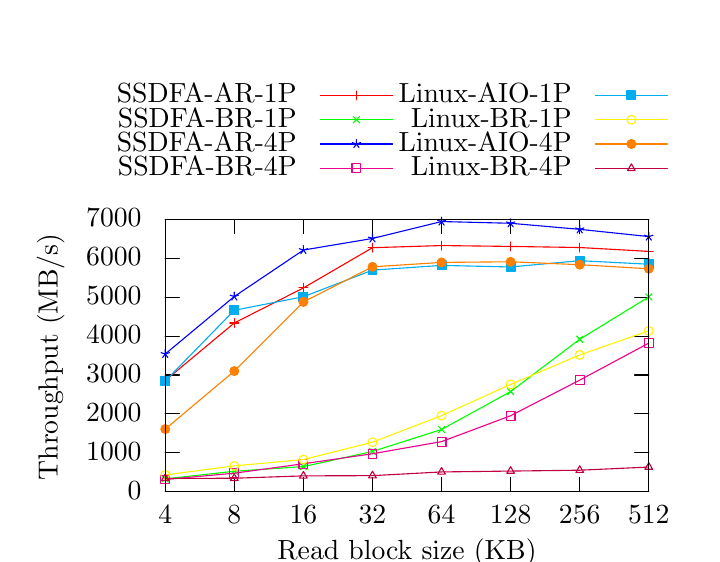
\begin{tikzpicture}[gnuplot]
%% generated with GNUPLOT 4.6p4 (Lua 5.1; terminal rev. 99, script rev. 100)
%% Wed 21 Oct 2015 09:54:35 PM EDT
\path (0.000,0.000) rectangle (8.382,6.350);
\gpcolor{color=gp lt color border}
\gpsetlinetype{gp lt border}
\gpsetlinewidth{1.00}
\draw[gp path] (1.688,0.985)--(1.868,0.985);
\draw[gp path] (7.829,0.985)--(7.649,0.985);
\node[gp node right] at (1.504,0.985) { 0};
\draw[gp path] (1.688,1.479)--(1.868,1.479);
\draw[gp path] (7.829,1.479)--(7.649,1.479);
\node[gp node right] at (1.504,1.479) { 1000};
\draw[gp path] (1.688,1.972)--(1.868,1.972);
\draw[gp path] (7.829,1.972)--(7.649,1.972);
\node[gp node right] at (1.504,1.972) { 2000};
\draw[gp path] (1.688,2.466)--(1.868,2.466);
\draw[gp path] (7.829,2.466)--(7.649,2.466);
\node[gp node right] at (1.504,2.466) { 3000};
\draw[gp path] (1.688,2.960)--(1.868,2.960);
\draw[gp path] (7.829,2.960)--(7.649,2.960);
\node[gp node right] at (1.504,2.960) { 4000};
\draw[gp path] (1.688,3.454)--(1.868,3.454);
\draw[gp path] (7.829,3.454)--(7.649,3.454);
\node[gp node right] at (1.504,3.454) { 5000};
\draw[gp path] (1.688,3.947)--(1.868,3.947);
\draw[gp path] (7.829,3.947)--(7.649,3.947);
\node[gp node right] at (1.504,3.947) { 6000};
\draw[gp path] (1.688,4.441)--(1.868,4.441);
\draw[gp path] (7.829,4.441)--(7.649,4.441);
\node[gp node right] at (1.504,4.441) { 7000};
\draw[gp path] (1.688,0.985)--(1.688,1.165);
\draw[gp path] (1.688,4.441)--(1.688,4.261);
\node[gp node center] at (1.688,0.677) {4};
\draw[gp path] (2.565,0.985)--(2.565,1.165);
\draw[gp path] (2.565,4.441)--(2.565,4.261);
\node[gp node center] at (2.565,0.677) {8};
\draw[gp path] (3.443,0.985)--(3.443,1.165);
\draw[gp path] (3.443,4.441)--(3.443,4.261);
\node[gp node center] at (3.443,0.677) {16};
\draw[gp path] (4.320,0.985)--(4.320,1.165);
\draw[gp path] (4.320,4.441)--(4.320,4.261);
\node[gp node center] at (4.320,0.677) {32};
\draw[gp path] (5.197,0.985)--(5.197,1.165);
\draw[gp path] (5.197,4.441)--(5.197,4.261);
\node[gp node center] at (5.197,0.677) {64};
\draw[gp path] (6.074,0.985)--(6.074,1.165);
\draw[gp path] (6.074,4.441)--(6.074,4.261);
\node[gp node center] at (6.074,0.677) {128};
\draw[gp path] (6.952,0.985)--(6.952,1.165);
\draw[gp path] (6.952,4.441)--(6.952,4.261);
\node[gp node center] at (6.952,0.677) {256};
\draw[gp path] (7.829,0.985)--(7.829,1.165);
\draw[gp path] (7.829,4.441)--(7.829,4.261);
\node[gp node center] at (7.829,0.677) {512};
\draw[gp path] (1.688,4.441)--(1.688,0.985)--(7.829,0.985)--(7.829,4.441)--cycle;
\node[gp node center,rotate=-270] at (0.246,2.713) {Throughput (MB/s)};
\node[gp node center] at (4.758,0.215) {Read block size (KB)};
\node[gp node right] at (3.474,6.016) {SSDFA-AR-1P};
\gpcolor{color=gp lt color 0}
\gpsetlinetype{gp lt plot 0}
\draw[gp path] (3.658,6.016)--(4.574,6.016);
\draw[gp path] (1.688,2.396)--(2.565,3.127)--(3.443,3.572)--(4.320,4.083)--(5.197,4.110)%
  --(6.074,4.099)--(6.952,4.085)--(7.829,4.036);
\gpsetpointsize{4.00}
\gppoint{gp mark 1}{(1.688,2.396)}
\gppoint{gp mark 1}{(2.565,3.127)}
\gppoint{gp mark 1}{(3.443,3.572)}
\gppoint{gp mark 1}{(4.320,4.083)}
\gppoint{gp mark 1}{(5.197,4.110)}
\gppoint{gp mark 1}{(6.074,4.099)}
\gppoint{gp mark 1}{(6.952,4.085)}
\gppoint{gp mark 1}{(7.829,4.036)}
\gppoint{gp mark 1}{(4.116,6.016)}
\gpcolor{color=gp lt color border}
\node[gp node right] at (3.474,5.708) {SSDFA-BR-1P};
\gpcolor{color=gp lt color 1}
\gpsetlinetype{gp lt plot 1}
\draw[gp path] (3.658,5.708)--(4.574,5.708);
\draw[gp path] (1.688,1.147)--(2.565,1.244)--(3.443,1.303)--(4.320,1.495)--(5.197,1.774)%
  --(6.074,2.255)--(6.952,2.920)--(7.829,3.457);
\gppoint{gp mark 2}{(1.688,1.147)}
\gppoint{gp mark 2}{(2.565,1.244)}
\gppoint{gp mark 2}{(3.443,1.303)}
\gppoint{gp mark 2}{(4.320,1.495)}
\gppoint{gp mark 2}{(5.197,1.774)}
\gppoint{gp mark 2}{(6.074,2.255)}
\gppoint{gp mark 2}{(6.952,2.920)}
\gppoint{gp mark 2}{(7.829,3.457)}
\gppoint{gp mark 2}{(4.116,5.708)}
\gpcolor{color=gp lt color border}
\node[gp node right] at (3.474,5.400) {SSDFA-AR-4P};
\gpcolor{color=gp lt color 2}
\gpsetlinetype{gp lt plot 2}
\draw[gp path] (3.658,5.400)--(4.574,5.400);
\draw[gp path] (1.688,2.733)--(2.565,3.463)--(3.443,4.053)--(4.320,4.200)--(5.197,4.415)%
  --(6.074,4.393)--(6.952,4.316)--(7.829,4.224);
\gppoint{gp mark 3}{(1.688,2.733)}
\gppoint{gp mark 3}{(2.565,3.463)}
\gppoint{gp mark 3}{(3.443,4.053)}
\gppoint{gp mark 3}{(4.320,4.200)}
\gppoint{gp mark 3}{(5.197,4.415)}
\gppoint{gp mark 3}{(6.074,4.393)}
\gppoint{gp mark 3}{(6.952,4.316)}
\gppoint{gp mark 3}{(7.829,4.224)}
\gppoint{gp mark 3}{(4.116,5.400)}
\gpcolor{color=gp lt color border}
\node[gp node right] at (3.474,5.092) {SSDFA-BR-4P};
\gpcolor{color=gp lt color 3}
\gpsetlinetype{gp lt plot 3}
\draw[gp path] (3.658,5.092)--(4.574,5.092);
\draw[gp path] (1.688,1.139)--(2.565,1.219)--(3.443,1.339)--(4.320,1.466)--(5.197,1.620)%
  --(6.074,1.949)--(6.952,2.401)--(7.829,2.871);
\gppoint{gp mark 4}{(1.688,1.139)}
\gppoint{gp mark 4}{(2.565,1.219)}
\gppoint{gp mark 4}{(3.443,1.339)}
\gppoint{gp mark 4}{(4.320,1.466)}
\gppoint{gp mark 4}{(5.197,1.620)}
\gppoint{gp mark 4}{(6.074,1.949)}
\gppoint{gp mark 4}{(6.952,2.401)}
\gppoint{gp mark 4}{(7.829,2.871)}
\gppoint{gp mark 4}{(4.116,5.092)}
\gpcolor{color=gp lt color border}
\node[gp node right] at (6.966,6.016) {Linux-AIO-1P};
\gpcolor{color=gp lt color 4}
\gpsetlinetype{gp lt plot 4}
\draw[gp path] (7.150,6.016)--(8.066,6.016);
\draw[gp path] (1.688,2.390)--(2.565,3.288)--(3.443,3.460)--(4.320,3.798)--(5.197,3.858)%
  --(6.074,3.838)--(6.952,3.918)--(7.829,3.873);
\gppoint{gp mark 5}{(1.688,2.390)}
\gppoint{gp mark 5}{(2.565,3.288)}
\gppoint{gp mark 5}{(3.443,3.460)}
\gppoint{gp mark 5}{(4.320,3.798)}
\gppoint{gp mark 5}{(5.197,3.858)}
\gppoint{gp mark 5}{(6.074,3.838)}
\gppoint{gp mark 5}{(6.952,3.918)}
\gppoint{gp mark 5}{(7.829,3.873)}
\gppoint{gp mark 5}{(7.608,6.016)}
\gpcolor{color=gp lt color border}
\node[gp node right] at (6.966,5.708) {Linux-BR-1P};
\gpcolor{color=gp lt color 5}
\gpsetlinetype{gp lt plot 5}
\draw[gp path] (7.150,5.708)--(8.066,5.708);
\draw[gp path] (1.688,1.197)--(2.565,1.312)--(3.443,1.392)--(4.320,1.613)--(5.197,1.950)%
  --(6.074,2.346)--(6.952,2.721)--(7.829,3.027);
\gppoint{gp mark 6}{(1.688,1.197)}
\gppoint{gp mark 6}{(2.565,1.312)}
\gppoint{gp mark 6}{(3.443,1.392)}
\gppoint{gp mark 6}{(4.320,1.613)}
\gppoint{gp mark 6}{(5.197,1.950)}
\gppoint{gp mark 6}{(6.074,2.346)}
\gppoint{gp mark 6}{(6.952,2.721)}
\gppoint{gp mark 6}{(7.829,3.027)}
\gppoint{gp mark 6}{(7.608,5.708)}
\gpcolor{color=gp lt color border}
\node[gp node right] at (6.966,5.400) {Linux-AIO-4P};
\gpcolor{color=gp lt color 6}
\gpsetlinetype{gp lt plot 6}
\draw[gp path] (7.150,5.400)--(8.066,5.400);
\draw[gp path] (1.688,1.779)--(2.565,2.516)--(3.443,3.394)--(4.320,3.840)--(5.197,3.896)%
  --(6.074,3.904)--(6.952,3.867)--(7.829,3.815);
\gppoint{gp mark 7}{(1.688,1.779)}
\gppoint{gp mark 7}{(2.565,2.516)}
\gppoint{gp mark 7}{(3.443,3.394)}
\gppoint{gp mark 7}{(4.320,3.840)}
\gppoint{gp mark 7}{(5.197,3.896)}
\gppoint{gp mark 7}{(6.074,3.904)}
\gppoint{gp mark 7}{(6.952,3.867)}
\gppoint{gp mark 7}{(7.829,3.815)}
\gppoint{gp mark 7}{(7.608,5.400)}
\gpcolor{color=gp lt color border}
\node[gp node right] at (6.966,5.092) {Linux-BR-4P};
\gpcolor{color=gp lt color 7}
\gpsetlinetype{gp lt plot 7}
\draw[gp path] (7.150,5.092)--(8.066,5.092);
\draw[gp path] (1.688,1.152)--(2.565,1.155)--(3.443,1.185)--(4.320,1.188)--(5.197,1.235)%
  --(6.074,1.246)--(6.952,1.257)--(7.829,1.297);
\gppoint{gp mark 8}{(1.688,1.152)}
\gppoint{gp mark 8}{(2.565,1.155)}
\gppoint{gp mark 8}{(3.443,1.185)}
\gppoint{gp mark 8}{(4.320,1.188)}
\gppoint{gp mark 8}{(5.197,1.235)}
\gppoint{gp mark 8}{(6.074,1.246)}
\gppoint{gp mark 8}{(6.952,1.257)}
\gppoint{gp mark 8}{(7.829,1.297)}
\gppoint{gp mark 8}{(7.608,5.092)}
\gpcolor{color=gp lt color border}
\gpsetlinetype{gp lt border}
\draw[gp path] (1.688,4.441)--(1.688,0.985)--(7.829,0.985)--(7.829,4.441)--cycle;
%% coordinates of the plot area
\gpdefrectangularnode{gp plot 1}{\pgfpoint{1.688cm}{0.985cm}}{\pgfpoint{7.829cm}{4.441cm}}
\end{tikzpicture}
%% gnuplot variables

\vspace{-15pt}
\caption{The read throughput of SSDFA and Linux solutions both on a single
processor and on four processors, measured by the N-1 test of IOR.
SSDFA-AR shows the throughput of asynchronous
read (no cache), SSDFA-BR shows the throughput of (synchronous) buffered read.
Linux-AIO and Linux-BR show the throughput of Linux AIO read and Linux
buffered read.}
\label{IOR-read}
\end{center}
\end{figure}

\begin{figure}[tb]
\begin{center}
\vspace{-15pt}
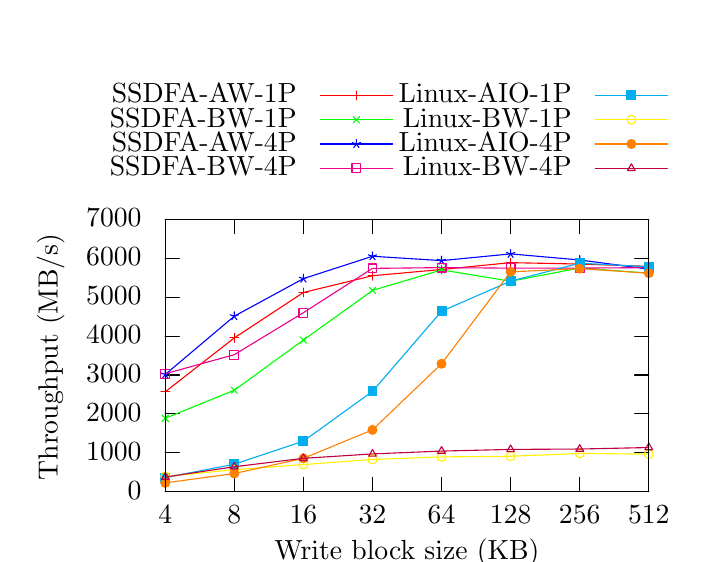
\begin{tikzpicture}[gnuplot]
%% generated with GNUPLOT 4.6p4 (Lua 5.1; terminal rev. 99, script rev. 100)
%% Wed 21 Oct 2015 09:54:51 PM EDT
\path (0.000,0.000) rectangle (8.382,6.350);
\gpcolor{color=gp lt color border}
\gpsetlinetype{gp lt border}
\gpsetlinewidth{1.00}
\draw[gp path] (1.688,0.985)--(1.868,0.985);
\draw[gp path] (7.829,0.985)--(7.649,0.985);
\node[gp node right] at (1.504,0.985) { 0};
\draw[gp path] (1.688,1.479)--(1.868,1.479);
\draw[gp path] (7.829,1.479)--(7.649,1.479);
\node[gp node right] at (1.504,1.479) { 1000};
\draw[gp path] (1.688,1.972)--(1.868,1.972);
\draw[gp path] (7.829,1.972)--(7.649,1.972);
\node[gp node right] at (1.504,1.972) { 2000};
\draw[gp path] (1.688,2.466)--(1.868,2.466);
\draw[gp path] (7.829,2.466)--(7.649,2.466);
\node[gp node right] at (1.504,2.466) { 3000};
\draw[gp path] (1.688,2.960)--(1.868,2.960);
\draw[gp path] (7.829,2.960)--(7.649,2.960);
\node[gp node right] at (1.504,2.960) { 4000};
\draw[gp path] (1.688,3.454)--(1.868,3.454);
\draw[gp path] (7.829,3.454)--(7.649,3.454);
\node[gp node right] at (1.504,3.454) { 5000};
\draw[gp path] (1.688,3.947)--(1.868,3.947);
\draw[gp path] (7.829,3.947)--(7.649,3.947);
\node[gp node right] at (1.504,3.947) { 6000};
\draw[gp path] (1.688,4.441)--(1.868,4.441);
\draw[gp path] (7.829,4.441)--(7.649,4.441);
\node[gp node right] at (1.504,4.441) { 7000};
\draw[gp path] (1.688,0.985)--(1.688,1.165);
\draw[gp path] (1.688,4.441)--(1.688,4.261);
\node[gp node center] at (1.688,0.677) {4};
\draw[gp path] (2.565,0.985)--(2.565,1.165);
\draw[gp path] (2.565,4.441)--(2.565,4.261);
\node[gp node center] at (2.565,0.677) {8};
\draw[gp path] (3.443,0.985)--(3.443,1.165);
\draw[gp path] (3.443,4.441)--(3.443,4.261);
\node[gp node center] at (3.443,0.677) {16};
\draw[gp path] (4.320,0.985)--(4.320,1.165);
\draw[gp path] (4.320,4.441)--(4.320,4.261);
\node[gp node center] at (4.320,0.677) {32};
\draw[gp path] (5.197,0.985)--(5.197,1.165);
\draw[gp path] (5.197,4.441)--(5.197,4.261);
\node[gp node center] at (5.197,0.677) {64};
\draw[gp path] (6.074,0.985)--(6.074,1.165);
\draw[gp path] (6.074,4.441)--(6.074,4.261);
\node[gp node center] at (6.074,0.677) {128};
\draw[gp path] (6.952,0.985)--(6.952,1.165);
\draw[gp path] (6.952,4.441)--(6.952,4.261);
\node[gp node center] at (6.952,0.677) {256};
\draw[gp path] (7.829,0.985)--(7.829,1.165);
\draw[gp path] (7.829,4.441)--(7.829,4.261);
\node[gp node center] at (7.829,0.677) {512};
\draw[gp path] (1.688,4.441)--(1.688,0.985)--(7.829,0.985)--(7.829,4.441)--cycle;
\node[gp node center,rotate=-270] at (0.246,2.713) {Throughput (MB/s)};
\node[gp node center] at (4.758,0.215) {Write block size (KB)};
\node[gp node right] at (3.474,6.016) {SSDFA-AW-1P};
\gpcolor{color=gp lt color 0}
\gpsetlinetype{gp lt plot 0}
\draw[gp path] (3.658,6.016)--(4.574,6.016);
\draw[gp path] (1.688,2.253)--(2.565,2.937)--(3.443,3.514)--(4.320,3.727)--(5.197,3.806)%
  --(6.074,3.893)--(6.952,3.875)--(7.829,3.846);
\gpsetpointsize{4.00}
\gppoint{gp mark 1}{(1.688,2.253)}
\gppoint{gp mark 1}{(2.565,2.937)}
\gppoint{gp mark 1}{(3.443,3.514)}
\gppoint{gp mark 1}{(4.320,3.727)}
\gppoint{gp mark 1}{(5.197,3.806)}
\gppoint{gp mark 1}{(6.074,3.893)}
\gppoint{gp mark 1}{(6.952,3.875)}
\gppoint{gp mark 1}{(7.829,3.846)}
\gppoint{gp mark 1}{(4.116,6.016)}
\gpcolor{color=gp lt color border}
\node[gp node right] at (3.474,5.708) {SSDFA-BW-1P};
\gpcolor{color=gp lt color 1}
\gpsetlinetype{gp lt plot 1}
\draw[gp path] (3.658,5.708)--(4.574,5.708);
\draw[gp path] (1.688,1.917)--(2.565,2.273)--(3.443,2.910)--(4.320,3.540)--(5.197,3.801)%
  --(6.074,3.657)--(6.952,3.825)--(7.829,3.759);
\gppoint{gp mark 2}{(1.688,1.917)}
\gppoint{gp mark 2}{(2.565,2.273)}
\gppoint{gp mark 2}{(3.443,2.910)}
\gppoint{gp mark 2}{(4.320,3.540)}
\gppoint{gp mark 2}{(5.197,3.801)}
\gppoint{gp mark 2}{(6.074,3.657)}
\gppoint{gp mark 2}{(6.952,3.825)}
\gppoint{gp mark 2}{(7.829,3.759)}
\gppoint{gp mark 2}{(4.116,5.708)}
\gpcolor{color=gp lt color border}
\node[gp node right] at (3.474,5.400) {SSDFA-AW-4P};
\gpcolor{color=gp lt color 2}
\gpsetlinetype{gp lt plot 2}
\draw[gp path] (3.658,5.400)--(4.574,5.400);
\draw[gp path] (1.688,2.473)--(2.565,3.213)--(3.443,3.690)--(4.320,3.974)--(5.197,3.919)%
  --(6.074,4.004)--(6.952,3.927)--(7.829,3.811);
\gppoint{gp mark 3}{(1.688,2.473)}
\gppoint{gp mark 3}{(2.565,3.213)}
\gppoint{gp mark 3}{(3.443,3.690)}
\gppoint{gp mark 3}{(4.320,3.974)}
\gppoint{gp mark 3}{(5.197,3.919)}
\gppoint{gp mark 3}{(6.074,4.004)}
\gppoint{gp mark 3}{(6.952,3.927)}
\gppoint{gp mark 3}{(7.829,3.811)}
\gppoint{gp mark 3}{(4.116,5.400)}
\gpcolor{color=gp lt color border}
\node[gp node right] at (3.474,5.092) {SSDFA-BW-4P};
\gpcolor{color=gp lt color 3}
\gpsetlinetype{gp lt plot 3}
\draw[gp path] (3.658,5.092)--(4.574,5.092);
\draw[gp path] (1.688,2.482)--(2.565,2.724)--(3.443,3.258)--(4.320,3.820)--(5.197,3.830)%
  --(6.074,3.823)--(6.952,3.824)--(7.829,3.830);
\gppoint{gp mark 4}{(1.688,2.482)}
\gppoint{gp mark 4}{(2.565,2.724)}
\gppoint{gp mark 4}{(3.443,3.258)}
\gppoint{gp mark 4}{(4.320,3.820)}
\gppoint{gp mark 4}{(5.197,3.830)}
\gppoint{gp mark 4}{(6.074,3.823)}
\gppoint{gp mark 4}{(6.952,3.824)}
\gppoint{gp mark 4}{(7.829,3.830)}
\gppoint{gp mark 4}{(4.116,5.092)}
\gpcolor{color=gp lt color border}
\node[gp node right] at (6.966,6.016) {Linux-AIO-1P};
\gpcolor{color=gp lt color 4}
\gpsetlinetype{gp lt plot 4}
\draw[gp path] (7.150,6.016)--(8.066,6.016);
\draw[gp path] (1.688,1.163)--(2.565,1.333)--(3.443,1.626)--(4.320,2.258)--(5.197,3.276)%
  --(6.074,3.658)--(6.952,3.886)--(7.829,3.841);
\gppoint{gp mark 5}{(1.688,1.163)}
\gppoint{gp mark 5}{(2.565,1.333)}
\gppoint{gp mark 5}{(3.443,1.626)}
\gppoint{gp mark 5}{(4.320,2.258)}
\gppoint{gp mark 5}{(5.197,3.276)}
\gppoint{gp mark 5}{(6.074,3.658)}
\gppoint{gp mark 5}{(6.952,3.886)}
\gppoint{gp mark 5}{(7.829,3.841)}
\gppoint{gp mark 5}{(7.608,6.016)}
\gpcolor{color=gp lt color border}
\node[gp node right] at (6.966,5.708) {Linux-BW-1P};
\gpcolor{color=gp lt color 5}
\gpsetlinetype{gp lt plot 5}
\draw[gp path] (7.150,5.708)--(8.066,5.708);
\draw[gp path] (1.688,1.178)--(2.565,1.263)--(3.443,1.329)--(4.320,1.393)--(5.197,1.426)%
  --(6.074,1.434)--(6.952,1.470)--(7.829,1.461);
\gppoint{gp mark 6}{(1.688,1.178)}
\gppoint{gp mark 6}{(2.565,1.263)}
\gppoint{gp mark 6}{(3.443,1.329)}
\gppoint{gp mark 6}{(4.320,1.393)}
\gppoint{gp mark 6}{(5.197,1.426)}
\gppoint{gp mark 6}{(6.074,1.434)}
\gppoint{gp mark 6}{(6.952,1.470)}
\gppoint{gp mark 6}{(7.829,1.461)}
\gppoint{gp mark 6}{(7.608,5.708)}
\gpcolor{color=gp lt color border}
\node[gp node right] at (6.966,5.400) {Linux-AIO-4P};
\gpcolor{color=gp lt color 6}
\gpsetlinetype{gp lt plot 6}
\draw[gp path] (7.150,5.400)--(8.066,5.400);
\draw[gp path] (1.688,1.096)--(2.565,1.215)--(3.443,1.408)--(4.320,1.769)--(5.197,2.609)%
  --(6.074,3.776)--(6.952,3.817)--(7.829,3.759);
\gppoint{gp mark 7}{(1.688,1.096)}
\gppoint{gp mark 7}{(2.565,1.215)}
\gppoint{gp mark 7}{(3.443,1.408)}
\gppoint{gp mark 7}{(4.320,1.769)}
\gppoint{gp mark 7}{(5.197,2.609)}
\gppoint{gp mark 7}{(6.074,3.776)}
\gppoint{gp mark 7}{(6.952,3.817)}
\gppoint{gp mark 7}{(7.829,3.759)}
\gppoint{gp mark 7}{(7.608,5.400)}
\gpcolor{color=gp lt color border}
\node[gp node right] at (6.966,5.092) {Linux-BW-4P};
\gpcolor{color=gp lt color 7}
\gpsetlinetype{gp lt plot 7}
\draw[gp path] (7.150,5.092)--(8.066,5.092);
\draw[gp path] (1.688,1.170)--(2.565,1.301)--(3.443,1.408)--(4.320,1.464)--(5.197,1.500)%
  --(6.074,1.521)--(6.952,1.526)--(7.829,1.545);
\gppoint{gp mark 8}{(1.688,1.170)}
\gppoint{gp mark 8}{(2.565,1.301)}
\gppoint{gp mark 8}{(3.443,1.408)}
\gppoint{gp mark 8}{(4.320,1.464)}
\gppoint{gp mark 8}{(5.197,1.500)}
\gppoint{gp mark 8}{(6.074,1.521)}
\gppoint{gp mark 8}{(6.952,1.526)}
\gppoint{gp mark 8}{(7.829,1.545)}
\gppoint{gp mark 8}{(7.608,5.092)}
\gpcolor{color=gp lt color border}
\gpsetlinetype{gp lt border}
\draw[gp path] (1.688,4.441)--(1.688,0.985)--(7.829,0.985)--(7.829,4.441)--cycle;
%% coordinates of the plot area
\gpdefrectangularnode{gp plot 1}{\pgfpoint{1.688cm}{0.985cm}}{\pgfpoint{7.829cm}{4.441cm}}
\end{tikzpicture}
%% gnuplot variables

\vspace{-15pt}
\caption{The write throughput of SSDFA and Linux solutions both on
a single processor and on four processors, measured by the N-1 test of IOR.
SSDFA-AW shows the throughput of asynchronous write
(no cache), SSDFA-BW shows the throughput of SSDFA (synchronous) buffered write.
Linux-AIO and Linux-BW shows the throughput of Linux AIO write and Linux
buffered write.}
\label{IOR-write}
\end{center}
\end{figure}

\begin{figure}[tb]
\begin{center}
\vspace{-15pt}
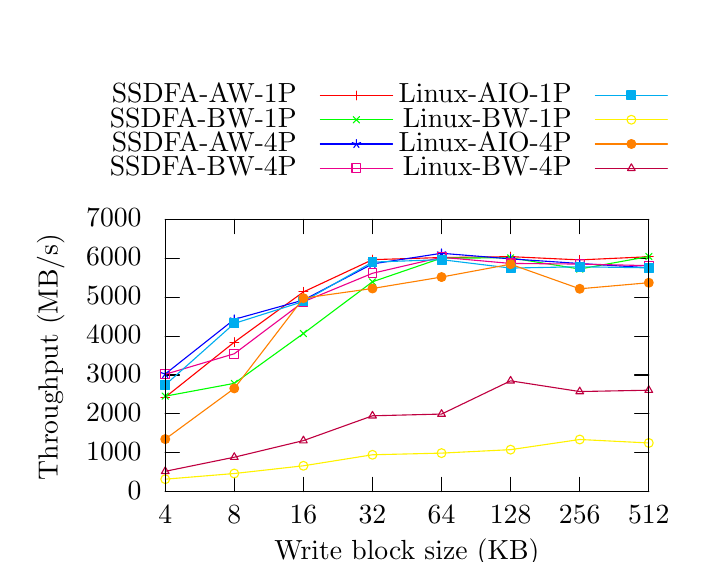
\begin{tikzpicture}[gnuplot]
%% generated with GNUPLOT 4.6p4 (Lua 5.1; terminal rev. 99, script rev. 100)
%% Wed 21 Oct 2015 09:55:00 PM EDT
\path (0.000,0.000) rectangle (8.382,6.350);
\gpcolor{color=gp lt color border}
\gpsetlinetype{gp lt border}
\gpsetlinewidth{1.00}
\draw[gp path] (1.688,0.985)--(1.868,0.985);
\draw[gp path] (7.829,0.985)--(7.649,0.985);
\node[gp node right] at (1.504,0.985) { 0};
\draw[gp path] (1.688,1.479)--(1.868,1.479);
\draw[gp path] (7.829,1.479)--(7.649,1.479);
\node[gp node right] at (1.504,1.479) { 1000};
\draw[gp path] (1.688,1.972)--(1.868,1.972);
\draw[gp path] (7.829,1.972)--(7.649,1.972);
\node[gp node right] at (1.504,1.972) { 2000};
\draw[gp path] (1.688,2.466)--(1.868,2.466);
\draw[gp path] (7.829,2.466)--(7.649,2.466);
\node[gp node right] at (1.504,2.466) { 3000};
\draw[gp path] (1.688,2.960)--(1.868,2.960);
\draw[gp path] (7.829,2.960)--(7.649,2.960);
\node[gp node right] at (1.504,2.960) { 4000};
\draw[gp path] (1.688,3.454)--(1.868,3.454);
\draw[gp path] (7.829,3.454)--(7.649,3.454);
\node[gp node right] at (1.504,3.454) { 5000};
\draw[gp path] (1.688,3.947)--(1.868,3.947);
\draw[gp path] (7.829,3.947)--(7.649,3.947);
\node[gp node right] at (1.504,3.947) { 6000};
\draw[gp path] (1.688,4.441)--(1.868,4.441);
\draw[gp path] (7.829,4.441)--(7.649,4.441);
\node[gp node right] at (1.504,4.441) { 7000};
\draw[gp path] (1.688,0.985)--(1.688,1.165);
\draw[gp path] (1.688,4.441)--(1.688,4.261);
\node[gp node center] at (1.688,0.677) {4};
\draw[gp path] (2.565,0.985)--(2.565,1.165);
\draw[gp path] (2.565,4.441)--(2.565,4.261);
\node[gp node center] at (2.565,0.677) {8};
\draw[gp path] (3.443,0.985)--(3.443,1.165);
\draw[gp path] (3.443,4.441)--(3.443,4.261);
\node[gp node center] at (3.443,0.677) {16};
\draw[gp path] (4.320,0.985)--(4.320,1.165);
\draw[gp path] (4.320,4.441)--(4.320,4.261);
\node[gp node center] at (4.320,0.677) {32};
\draw[gp path] (5.197,0.985)--(5.197,1.165);
\draw[gp path] (5.197,4.441)--(5.197,4.261);
\node[gp node center] at (5.197,0.677) {64};
\draw[gp path] (6.074,0.985)--(6.074,1.165);
\draw[gp path] (6.074,4.441)--(6.074,4.261);
\node[gp node center] at (6.074,0.677) {128};
\draw[gp path] (6.952,0.985)--(6.952,1.165);
\draw[gp path] (6.952,4.441)--(6.952,4.261);
\node[gp node center] at (6.952,0.677) {256};
\draw[gp path] (7.829,0.985)--(7.829,1.165);
\draw[gp path] (7.829,4.441)--(7.829,4.261);
\node[gp node center] at (7.829,0.677) {512};
\draw[gp path] (1.688,4.441)--(1.688,0.985)--(7.829,0.985)--(7.829,4.441)--cycle;
\node[gp node center,rotate=-270] at (0.246,2.713) {Throughput (MB/s)};
\node[gp node center] at (4.758,0.215) {Write block size (KB)};
\node[gp node right] at (3.474,6.016) {SSDFA-AW-1P};
\gpcolor{color=gp lt color 0}
\gpsetlinetype{gp lt plot 0}
\draw[gp path] (3.658,6.016)--(4.574,6.016);
\draw[gp path] (1.688,2.184)--(2.565,2.883)--(3.443,3.521)--(4.320,3.931)--(5.197,3.958)%
  --(6.074,3.969)--(6.952,3.928)--(7.829,3.968);
\gpsetpointsize{4.00}
\gppoint{gp mark 1}{(1.688,2.184)}
\gppoint{gp mark 1}{(2.565,2.883)}
\gppoint{gp mark 1}{(3.443,3.521)}
\gppoint{gp mark 1}{(4.320,3.931)}
\gppoint{gp mark 1}{(5.197,3.958)}
\gppoint{gp mark 1}{(6.074,3.969)}
\gppoint{gp mark 1}{(6.952,3.928)}
\gppoint{gp mark 1}{(7.829,3.968)}
\gppoint{gp mark 1}{(4.116,6.016)}
\gpcolor{color=gp lt color border}
\node[gp node right] at (3.474,5.708) {SSDFA-BW-1P};
\gpcolor{color=gp lt color 1}
\gpsetlinetype{gp lt plot 1}
\draw[gp path] (3.658,5.708)--(4.574,5.708);
\draw[gp path] (1.688,2.197)--(2.565,2.360)--(3.443,2.993)--(4.320,3.650)--(5.197,3.951)%
  --(6.074,3.954)--(6.952,3.812)--(7.829,3.971);
\gppoint{gp mark 2}{(1.688,2.197)}
\gppoint{gp mark 2}{(2.565,2.360)}
\gppoint{gp mark 2}{(3.443,2.993)}
\gppoint{gp mark 2}{(4.320,3.650)}
\gppoint{gp mark 2}{(5.197,3.951)}
\gppoint{gp mark 2}{(6.074,3.954)}
\gppoint{gp mark 2}{(6.952,3.812)}
\gppoint{gp mark 2}{(7.829,3.971)}
\gppoint{gp mark 2}{(4.116,5.708)}
\gpcolor{color=gp lt color border}
\node[gp node right] at (3.474,5.400) {SSDFA-AW-4P};
\gpcolor{color=gp lt color 2}
\gpsetlinetype{gp lt plot 2}
\draw[gp path] (3.658,5.400)--(4.574,5.400);
\draw[gp path] (1.688,2.479)--(2.565,3.173)--(3.443,3.418)--(4.320,3.877)--(5.197,4.012)%
  --(6.074,3.941)--(6.952,3.882)--(7.829,3.828);
\gppoint{gp mark 3}{(1.688,2.479)}
\gppoint{gp mark 3}{(2.565,3.173)}
\gppoint{gp mark 3}{(3.443,3.418)}
\gppoint{gp mark 3}{(4.320,3.877)}
\gppoint{gp mark 3}{(5.197,4.012)}
\gppoint{gp mark 3}{(6.074,3.941)}
\gppoint{gp mark 3}{(6.952,3.882)}
\gppoint{gp mark 3}{(7.829,3.828)}
\gppoint{gp mark 3}{(4.116,5.400)}
\gpcolor{color=gp lt color border}
\node[gp node right] at (3.474,5.092) {SSDFA-BW-4P};
\gpcolor{color=gp lt color 3}
\gpsetlinetype{gp lt plot 3}
\draw[gp path] (3.658,5.092)--(4.574,5.092);
\draw[gp path] (1.688,2.475)--(2.565,2.736)--(3.443,3.396)--(4.320,3.758)--(5.197,3.961)%
  --(6.074,3.883)--(6.952,3.875)--(7.829,3.855);
\gppoint{gp mark 4}{(1.688,2.475)}
\gppoint{gp mark 4}{(2.565,2.736)}
\gppoint{gp mark 4}{(3.443,3.396)}
\gppoint{gp mark 4}{(4.320,3.758)}
\gppoint{gp mark 4}{(5.197,3.961)}
\gppoint{gp mark 4}{(6.074,3.883)}
\gppoint{gp mark 4}{(6.952,3.875)}
\gppoint{gp mark 4}{(7.829,3.855)}
\gppoint{gp mark 4}{(4.116,5.092)}
\gpcolor{color=gp lt color border}
\node[gp node right] at (6.966,6.016) {Linux-AIO-1P};
\gpcolor{color=gp lt color 4}
\gpsetlinetype{gp lt plot 4}
\draw[gp path] (7.150,6.016)--(8.066,6.016);
\draw[gp path] (1.688,2.340)--(2.565,3.121)--(3.443,3.400)--(4.320,3.900)--(5.197,3.931)%
  --(6.074,3.824)--(6.952,3.841)--(7.829,3.827);
\gppoint{gp mark 5}{(1.688,2.340)}
\gppoint{gp mark 5}{(2.565,3.121)}
\gppoint{gp mark 5}{(3.443,3.400)}
\gppoint{gp mark 5}{(4.320,3.900)}
\gppoint{gp mark 5}{(5.197,3.931)}
\gppoint{gp mark 5}{(6.074,3.824)}
\gppoint{gp mark 5}{(6.952,3.841)}
\gppoint{gp mark 5}{(7.829,3.827)}
\gppoint{gp mark 5}{(7.608,6.016)}
\gpcolor{color=gp lt color border}
\node[gp node right] at (6.966,5.708) {Linux-BW-1P};
\gpcolor{color=gp lt color 5}
\gpsetlinetype{gp lt plot 5}
\draw[gp path] (7.150,5.708)--(8.066,5.708);
\draw[gp path] (1.688,1.143)--(2.565,1.215)--(3.443,1.313)--(4.320,1.453)--(5.197,1.474)%
  --(6.074,1.518)--(6.952,1.647)--(7.829,1.603);
\gppoint{gp mark 6}{(1.688,1.143)}
\gppoint{gp mark 6}{(2.565,1.215)}
\gppoint{gp mark 6}{(3.443,1.313)}
\gppoint{gp mark 6}{(4.320,1.453)}
\gppoint{gp mark 6}{(5.197,1.474)}
\gppoint{gp mark 6}{(6.074,1.518)}
\gppoint{gp mark 6}{(6.952,1.647)}
\gppoint{gp mark 6}{(7.829,1.603)}
\gppoint{gp mark 6}{(7.608,5.708)}
\gpcolor{color=gp lt color border}
\node[gp node right] at (6.966,5.400) {Linux-AIO-4P};
\gpcolor{color=gp lt color 6}
\gpsetlinetype{gp lt plot 6}
\draw[gp path] (7.150,5.400)--(8.066,5.400);
\draw[gp path] (1.688,1.652)--(2.565,2.296)--(3.443,3.442)--(4.320,3.565)--(5.197,3.710)%
  --(6.074,3.873)--(6.952,3.561)--(7.829,3.638);
\gppoint{gp mark 7}{(1.688,1.652)}
\gppoint{gp mark 7}{(2.565,2.296)}
\gppoint{gp mark 7}{(3.443,3.442)}
\gppoint{gp mark 7}{(4.320,3.565)}
\gppoint{gp mark 7}{(5.197,3.710)}
\gppoint{gp mark 7}{(6.074,3.873)}
\gppoint{gp mark 7}{(6.952,3.561)}
\gppoint{gp mark 7}{(7.829,3.638)}
\gppoint{gp mark 7}{(7.608,5.400)}
\gpcolor{color=gp lt color border}
\node[gp node right] at (6.966,5.092) {Linux-BW-4P};
\gpcolor{color=gp lt color 7}
\gpsetlinetype{gp lt plot 7}
\draw[gp path] (7.150,5.092)--(8.066,5.092);
\draw[gp path] (1.688,1.243)--(2.565,1.422)--(3.443,1.633)--(4.320,1.948)--(5.197,1.970)%
  --(6.074,2.392)--(6.952,2.256)--(7.829,2.273);
\gppoint{gp mark 8}{(1.688,1.243)}
\gppoint{gp mark 8}{(2.565,1.422)}
\gppoint{gp mark 8}{(3.443,1.633)}
\gppoint{gp mark 8}{(4.320,1.948)}
\gppoint{gp mark 8}{(5.197,1.970)}
\gppoint{gp mark 8}{(6.074,2.392)}
\gppoint{gp mark 8}{(6.952,2.256)}
\gppoint{gp mark 8}{(7.829,2.273)}
\gppoint{gp mark 8}{(7.608,5.092)}
\gpcolor{color=gp lt color border}
\gpsetlinetype{gp lt border}
\draw[gp path] (1.688,4.441)--(1.688,0.985)--(7.829,0.985)--(7.829,4.441)--cycle;
%% coordinates of the plot area
\gpdefrectangularnode{gp plot 1}{\pgfpoint{1.688cm}{0.985cm}}{\pgfpoint{7.829cm}{4.441cm}}
\end{tikzpicture}
%% gnuplot variables

\vspace{-15pt}
\caption{The write throughput of SSDFA and Linux solutions both on
a single processor and on four processors, measured by the N-N test of IOR.
SSDFA-AW shows the throughput of asynchronous write
(no cache), SSDFA-BW shows the throughput of SSDFA (synchronous) buffered write.
Linux-AIO and Linux-BW shows the throughput of Linux AIO write and Linux
buffered write.}
\label{IOR-write-FPP}
\end{center}
\end{figure}

Figure \ref{IOR-read} shows that SSDFA read significantly outperforms
Linux read on a NUMA machine in the N-1 test. When
the request size is small, Linux AIO read has much
lower throughput than SSDFA asynchronous read (no cache) in the NUMA configuration
due to the bottleneck in the Linux software RAID. Although SSDFA synchronous
buffered read perform poorly with small request sizes, its throughput
increases constantly with larger requests. The throughput of Linux buffered read
in the NUMA configuration, on the other hand, barely increases with the
request size due to the high cache overhead.

SSDFA write performs much better than all Linux's solutions in the N-1 test,
especially for small request sizes (Figure \ref{IOR-write}). Thanks to
our novel design of the flush thread in our page cache, SSDFA synchronous
buffered write can achieve performance close to SSDFA asynchronous write.
XFS has two exclusive locks on each file: one is to protect the inode data
structure and is held briefly at each acquisition; the other is
to protect I/O access to the file and is held for a longer time. Linux
AIO write only acquires the one for inode and Linux buffered write acquires
both locks. Thus, Linux AIO cannot perform well with small writes on XFS,
but it can still reach maximal performance with a large request size on both
a single processor and four processors. Linux buffered write, on the other
hand, performs much worse and its performance can only be improved slightly
with a larger request size.

Figure \ref{IOR-write-FPP} shows that XFS and Linux page cache perform
better in the N-N test than in the N-1 test, but SSDFA can still outperform them,
especially
for synchronous write. The N-N test essentially removes nearly all lock
contention in XFS and Linux page cache, which boosts their performance.
However, the bottleneck in the Linux software RAID still exists, so like
the N-1 test, Linux AIO write is still slower than SSDFA asynchronous
write in the NUMA configuration. Again, SSDFA synchronous buffered write
can significantly outperform Linux buffered write thanks to our new design
of the flush thread. Linux buffered write on a single processor
performs worse than on four processors because Linux page cache hits
a bottleneck in page allocation on a single processor. When a dedicated
per-processor kernel thread cannot free sufficient pages to keep
up the speed of page allocation required by other threads, all threads
have to try to free pages and causes extremely high lock contention.

\section{Conclusion}
We present a storage system that achieves more than one million
random read IOPS based on a user-space file abstraction running
on an array of commodity SSDs.  The file abstraction builds on top of 
a local file system on each SSD in order to aggregates their IOPS.
It also creates dedicated threads for I/O to each SSD.  These threads
access the SSD and file exclusively, which eliminates lock contention 
in the file and device interfaces.
The design amplifies IOPS by 3.5 times and realizes nearly the 
full potential of the SSD hardware, less than 1\% loss for reads
and 2.4\% for writes.

In the file abstraction, we deploy a set-associative parallel
page cache designed for non-uniform memory architectures.  
The design divides the global page cache into many small, independent
sets, which reduces lock contention.  For NUMA architectures, the 
design minimizes the CPU overhead associated with remote memory copies 
through a hybrid SMP and message passing programming model. Each processor
is treated as a node in a distributed system and inter-processor operations
exchange messages through rendezvous queues served by a dedicated thread pool.
The multiple cores of each processor are programmed as an SMP.
With page caching, user-perceived throughput grows linearly with the 
cache hit rate up to 16 million IOPS, more than four times that realized
by Linux. Our optimizations in the parallel page cache achieve good performance
for all request sizes and synchronous write performs nearly as well as
asynchronous write.

As a whole, the design alleviates bottlenecks associated with lock contention,
CPU overhead, and remote memory copies across many layers of hardware and
software.  The design captures parallelism and non-uniform performance of
modern hardware to realize world-class performance for commodity SSDs.

\chapter{FlashGraph}
\label{sec:fg}
\chaptermark{FlashGraph: Processing Billion-Node Graphs on an Array of
Commodity SSDs}

This chapter describes FlashGraph, a general-purpose graph processing framework
built on top of SAFS for massive graphs. By utilizing commodity SSDs through SAFS,
FlashGraph enables a multicore server to process graphs with billions of vertices
and hundreds of billions of edges, with minimal performance loss. FlashGraph
processes graphs in a semi-external memory fashion, i.e., it stores vertex state
in memory and edge lists on SSDs. It hides latency by overlapping computation
with I/O. To save I/O bandwidth, FlashGraph only accesses edge lists requested
by applications from SSDs; to increase I/O throughput and reduce CPU overhead for I/O,
it conservatively merges I/O requests. These designs maximize performance
for applications with different I/O characteristics. FlashGraph exposes
a general and flexible vertex-centric programming interface that can express
a wide variety of graph algorithms and their optimizations. We demonstrate that
FlashGraph in semi-external memory performs many algorithms with performance
up to 80\% of its in-memory implementation and significantly outperforms
PowerGraph, a popular distributed in-memory graph engine.

\section{Introduction}
\input{FlashGraph/intro}

\section{Related Work}
\input{FlashGraph/relwork}

\input{FlashGraph/design}

\input{FlashGraph/eval}

\section{Conclusions}
\input{FlashGraph/conclusion}

\chapter{Sparse matrix multiplication}
\label{sec:fe}
\chaptermark{Semi-External Memory Sparse Matrix Multiplication on
Billion-node Graphs in a Multicore Architecture}

This chapter describes another view of graph analysis. Instead of viewing
a graph as a collection of vertices and edges, we encode a graph as
a sparse matrix and express graph analysis as matrix operations \cite{Mattson13}.
In this formulation, a row or a column of a sparse matrix represents a vertex
in a graph and a non-zero entry encodes the existence of an edge or the edge
weight on a graph. As such, many graph analysis algorithms such as PageRank
and spectral clustering are expressed as sparse matrix multiplication.
In this chapter, we describe an efficient implementation of sparse matrix
dense matrix multiplication (SpMM), a key operation for graph analysis. We
scale this matrix operation by utilizing commodity SSDs and implement it in
a semi-external memory (SEM) fashion, i.e., we keep the sparse matrix on SSDs
and dense matrices in memory. Our SEM SpMM incorporates many in-memory
optimizations that require a small memory footprint.
Coupled with many I/O optimizations, our SEM SpMM achieves performance
comparable to our in-memory implementation on a large parallel machine and
outperforms the implementations in Trilinos and Intel MKL.
Our experiments show that the SEM SpMM achieves almost 100\% performance
of the in-memory implementation on graphs when the dense matrix has more
than four columns; it achieves at least 65\% performance of the in-memory
implementation for all of our graphs when the dense matrix has only one column.
We apply our SpMM to three important graph analysis applications and show that
our SSD-based implementations can significantly outperform state of the art
of these applications and scale to billion-node graphs.

\section{Introduction}
\input{SpMM/intro}

\section{Related Work}
\input{SpMM/relwork}

\input{SpMM/design}

\input{SpMM/eval}

\section{Conclusions}
\input{SpMM/conclusion}

\chapter{FlashMatrix}
\label{sec:fm}
\chaptermark{FlashMatrix: Parallel, Scalable Data Analysis with Generalized
	Matrix Operations using Commodity SSDs}

This chapter describes FlashMatrix, a matrix-oriented programming framework
for general data analysis with high-level functional programming interface.
FlashMatrix incorporates the efficient sparse matrix multiplication in Chapter
\ref{sec:fe}. In this chapter, we focus on dense matrix operations in FlashMatrix.
To achieve generality, it provides a small number of generalized matrix
operations (GenOps) and reimplements a large number of matrix operations in
the R framework with GenOps. As such, it executes R code in parallel and out of
core automatically. FlashMatrix
uses vectorized user-defined functions (VUDF) to reduce the overhead of function
calls and fuses matrix operations to reduce data movement between CPU and
SSDs. We implement multiple machine learning algorithms in R to benchmark
the performance of FlashMatrix. The execution of the R implementations in
FlashMatrix has performance comparable to optimized C implementations.
When scaling beyond memory capacity on a large parallel machine, the out-of-core
execution of these R implementations in FlashMatrix has performance comparable
to in-memory execution on a billion-scale dataset. Both in-memory and
out-of-core execution significantly outperform the in-memory execution of
Spark MLlib.

\section{Introduction}
\input{FlashMatrix/intro}

\section{Related Work}
\input{FlashMatrix/relwork}

\input{FlashMatrix/design}

\input{FlashMatrix/eval}

\section{Conclusions}
\input{FlashMatrix/conclusion}

\chapter{Conclusion}
\label{sec:conclu}
\chaptermark{}



%\input{appendix}

%% REFERENCES

% if you use BIBTEX
\bibliographystyle{IEEEtran}
\bibliography{thesis}

\begin{vita}

%\begin{wrapfigure}{l}{0pt}
%\includegraphics[width=2in,height=2.5in,clip,keepaspectratio]{rjvheadshot.jpg}
%\end{wrapfigure}


\end{vita}
\end{document}
